% cSpell: disable

% Ignore the next line...
% \documentclass[UTF8,fontset=none,leqno]{ctexart}

% Make sure you have installed the fonts I use. If not, just remember to
% make some modifications.
\documentclass[UTF8,fontset=none,twoside,leqno,a4paper]{ctexart}
% \documentclass[UTF8,twoside,leqno]{ctexart}
\usepackage{amssymb}
\usepackage{amsmath}
% Add hyperlinks to the table of contents
\usepackage[hidelinks]{hyperref}
\usepackage{pdfpages}
\usepackage{bookmark}
\usepackage{xcolor}
% \definecolor{bb}{RGB}{251,114,153}

% \usepackage{lipsum}

% Enable unicode-math? If this is enabled, many font packages will not work.
% However, if this is enabled, the symbols look better.
\usepackage{unicode-math}
\setmathfont{Latin Modern Math}
\setmathfont{TeX Gyre Termes Math}[range=bb/{latin,Latin}]

\providecommand{\newsection}{}
\renewcommand{\newsection}{\cleardoublepage \thispagestyle{empty}}
% \renewcommand{\newsection}{\cleardoublepage \thispagestyle{plain}}

% ================================================================================
% Set the fonts. You can use whatever you like, or simply remove this part
% and remove the option "fontset=none".

\def\heiti{\CJKfontspec{Sarasa Mono SC Light}}
\def\songti{\CJKfontspec{Source Han Serif CN}}
\def\kaishu{\CJKfontspec{Sarasa Mono SC Light}}
\def\fangsong{\CJKfontspec{Sarasa Mono SC Light}}
\setmonofont{Sarasa Mono SC Light}
\setsansfont{Source Sans Pro Light}
\setCJKmonofont{Sarasa Mono SC Light}
\setCJKmainfont[ItalicFont=Sarasa Mono SC Light]{Source Han Serif CN}
\setCJKsansfont{Sarasa Mono SC Light}
% I use Sarasa Mono SC instead of Kaishu or Fangsong.
% The operating system I use do not have the 4 fonts:
% Heiti, Songti, Kaishu, Fangsong.

% ================================================================================

% Punctuation style: narrow some punctuation symbols
\punctstyle{kaiming}

% Footnote
% Footnotes per page
\usepackage[perpage]{footmisc}
% Define a new set of footnote symbols
\DefineFNsymbols*{myFootnoteStyle}{
    % If unicode-math is not enabled, the dollar signs can be removed.
    {$\dagger$}{$\ddagger$}{$\S$}{$\P$}{$\parallel$}{$\dagger\dagger$}{$\ddagger\ddagger$}
}
\setfnsymbol{myFootnoteStyle}
\renewcommand{\thefootnote}{\fnsymbol{footnote}}

% My own footnote command
\providecommand{\myFN}{}
\renewcommand{\myFN}[1]{\footnote{\sffamily \ #1}}

% Deprecated. Now I use the theorem layout
% Numbering style for exercises
% \usepackage{enumitem}
% \renewcommand{\labelenumi}{\textbf{\theenumi.}}
% \setlist[enumerate]{
%   leftmargin=0em,
%   listparindent=\parindent,
%   itemindent=*,
%   labelindent=\parindent,
%   align=left,
%   parsep=\parskip
% }

% Proof and solution style
\usepackage{amsthm}
% Use \nopunct to remove the dot: https://tex.stackexchange.com/questions/268912/can-i-change-the-dot-to-a-colon-after-proof-in-amsthm
% Use \vspace{-\topsep} to remove extra line: https://tex.stackexchange.com/questions/59755/space-before-proof
% \newenvironment{pf}{\begin{proof}[\indent\bf 证 \hspace{-.1em}\hspace{-\labelsep}\hspace{1em}\nopunct]\vspace{-\topsep}}{\end{proof}}
% \newenvironment{solution}{\begin{proof}[\indent\bf 解 \hspace{-.1em}\hspace{-\labelsep}\hspace{1em}\nopunct]\vspace{-\topsep}}{\end{proof}}
% \newenvironment{pas}{\begin{proof}[\indent\bf 证明与解 \hspace{-.1em}\hspace{-\labelsep}\hspace{1em}\nopunct]\vspace{-\topsep}}{\end{proof}}
\newenvironment{pf}{\begin{proof}[\indent\bf 证 \hspace{-.1em}\hspace{-\labelsep}\hspace{1em}\nopunct]}{\end{proof}}
\newenvironment{solution}{\begin{proof}[\indent\bf 解 \hspace{-.1em}\hspace{-\labelsep}\hspace{1em}\nopunct]}{\end{proof}}
\newenvironment{pas}{\begin{proof}[\indent\bf 证明与解 \hspace{-.1em}\hspace{-\labelsep}\hspace{1em}\nopunct]}{\end{proof}}

\newtheoremstyle{exer} % ⟨name⟩
{} % ⟨Space above⟩
{} % ⟨Space below⟩
{} % ⟨Body font⟩
{\parindent} % ⟨Indent amount⟩
{\bfseries} % ⟨Theorem head font⟩
{.} % ⟨Punctuation after theorem head⟩
{.5em} % ⟨Space after theorem head⟩
{} % ⟨Theorem head spec (can be left empty, meaning 'normal')⟩
\theoremstyle{exer}
\newtheorem{exercise}{}[subsection]

\newtheoremstyle{exer*} % ⟨name⟩
{} % ⟨Space above⟩
{} % ⟨Space below⟩
{} % ⟨Body font⟩
{\parindent} % ⟨Indent amount⟩
{\bfseries} % ⟨Theorem head font⟩
{} % ⟨Punctuation after theorem head⟩
{0em} % ⟨Space after theorem head⟩
{} % ⟨Theorem head spec (can be left empty, meaning 'normal')⟩
\theoremstyle{exer*}
\newtheorem*{exercise*}{}

\newtheoremstyle{remarkStyle} % ⟨name⟩
{} % ⟨Space above⟩
{} % ⟨Space below⟩
{} % ⟨Body font⟩
{\parindent} % ⟨Indent amount⟩
{\bfseries} % ⟨Theorem head font⟩
{} % ⟨Punctuation after theorem head⟩
{1em} % ⟨Space after theorem head⟩
{} % ⟨Theorem head spec (can be left empty, meaning 'normal')⟩
\theoremstyle{remarkStyle}
\newtheorem*{supplement}{补充题}
\newtheorem*{proposition}{命题}
\newtheorem*{definition}{定义}
\newtheorem*{example}{例}
\newtheorem*{remark}{评注}

% https://oomake.com/question/175655
\renewcommand{\theexercise}{\arabic{exercise}}
% \newenvironment{pf}{\begin{proof}[\indent\bf 证 \hphantom{.\ }\nopunct]\vspace{-\topsep}}{\vspace{-\topsep}\end{proof}}
% \newenvironment{solution}{\begin{proof}[\indent\bf 解 \hphantom{.\ }\nopunct]\vspace{-\topsep}}{\vspace{-\topsep}\end{proof}}
% \newenvironment{pas}{\begin{proof}[\indent\bf 证明与解 \hphantom{.\ }\nopunct]\vspace{-\topsep}}{\vspace{-\topsep}\end{proof}}
% Use a black square instead
% \renewcommand{\qedsymbol}{$\blacksquare$}

% Use some special characters.
\usepackage{pifont}

% Allow page breaks in display formulae
\allowdisplaybreaks[4]

\def\CC{\mathbb{C}}
\def\RR{\mathbb{R}}
\def\QQ{\mathbb{Q}}
\def\ZZ{\mathbb{Z}}
\def\NN{\mathbb{N}}
\def\FF{\mathbb{F}}
\def\ii{\mathrm{i}}
\def\myStar{\ding{72}}
\def\ellipsis{\dots}
\def\period{\text{。}}
\def\qedsymbol{\ding{44}}
\newcommand{\term}[1]{(\textit{#1})}

\makeatletter
% \providecommand{\leqnomode}{}
% \renewcommand{\leqnomode}{\tagsleft@true\let\veqno\@@leqno}
% \providecommand{\reqnomode}{}
% \renewcommand{\reqnomode}{\tagsleft@false\let\veqno\@@eqno}

% Clear even-numbered pages
\renewcommand{\cleardoublepage}{\relax \clearpage
    \if@twoside \ifodd\c@page\relax
        \else \thispagestyle{empty} \ \clearpage\fi\fi}

% For two-sided documents
\renewcommand\ps@headings{%
    \let\@oddfoot\@empty\let\@evenfoot\@empty
    \def\@evenhead{\sffamily\thepage\hfil\slshape\leftmark}%
    \def\@oddhead{\sffamily{\slshape\rightmark}\hfil\thepage}%
    \let\@mkboth\markboth
    \def\sectionmark##1{%
        \markboth {{%
                    \ifnum \c@secnumdepth >\z@
                        \thesection\quad
                    \fi
                    ##1}}{}}%
    \def\mySubSectmark##1{%
        \markright {%
            \ifnum \c@secnumdepth >\@ne
                \thesubsection\quad
            \fi
            ##1}}}

\renewcommand\ps@plain{
    \let\@oddhead\@empty
    \def\@oddfoot{\hfil\sffamily\thepage\hfil}%
    \let\@evenhead\@empty
    \let\@evenfoot\@oddfoot}

\makeatother

% ============================================================
% The document begins.
% ============================================================

\begin{document}

% \pagestyle{empty}

\pagestyle{empty}
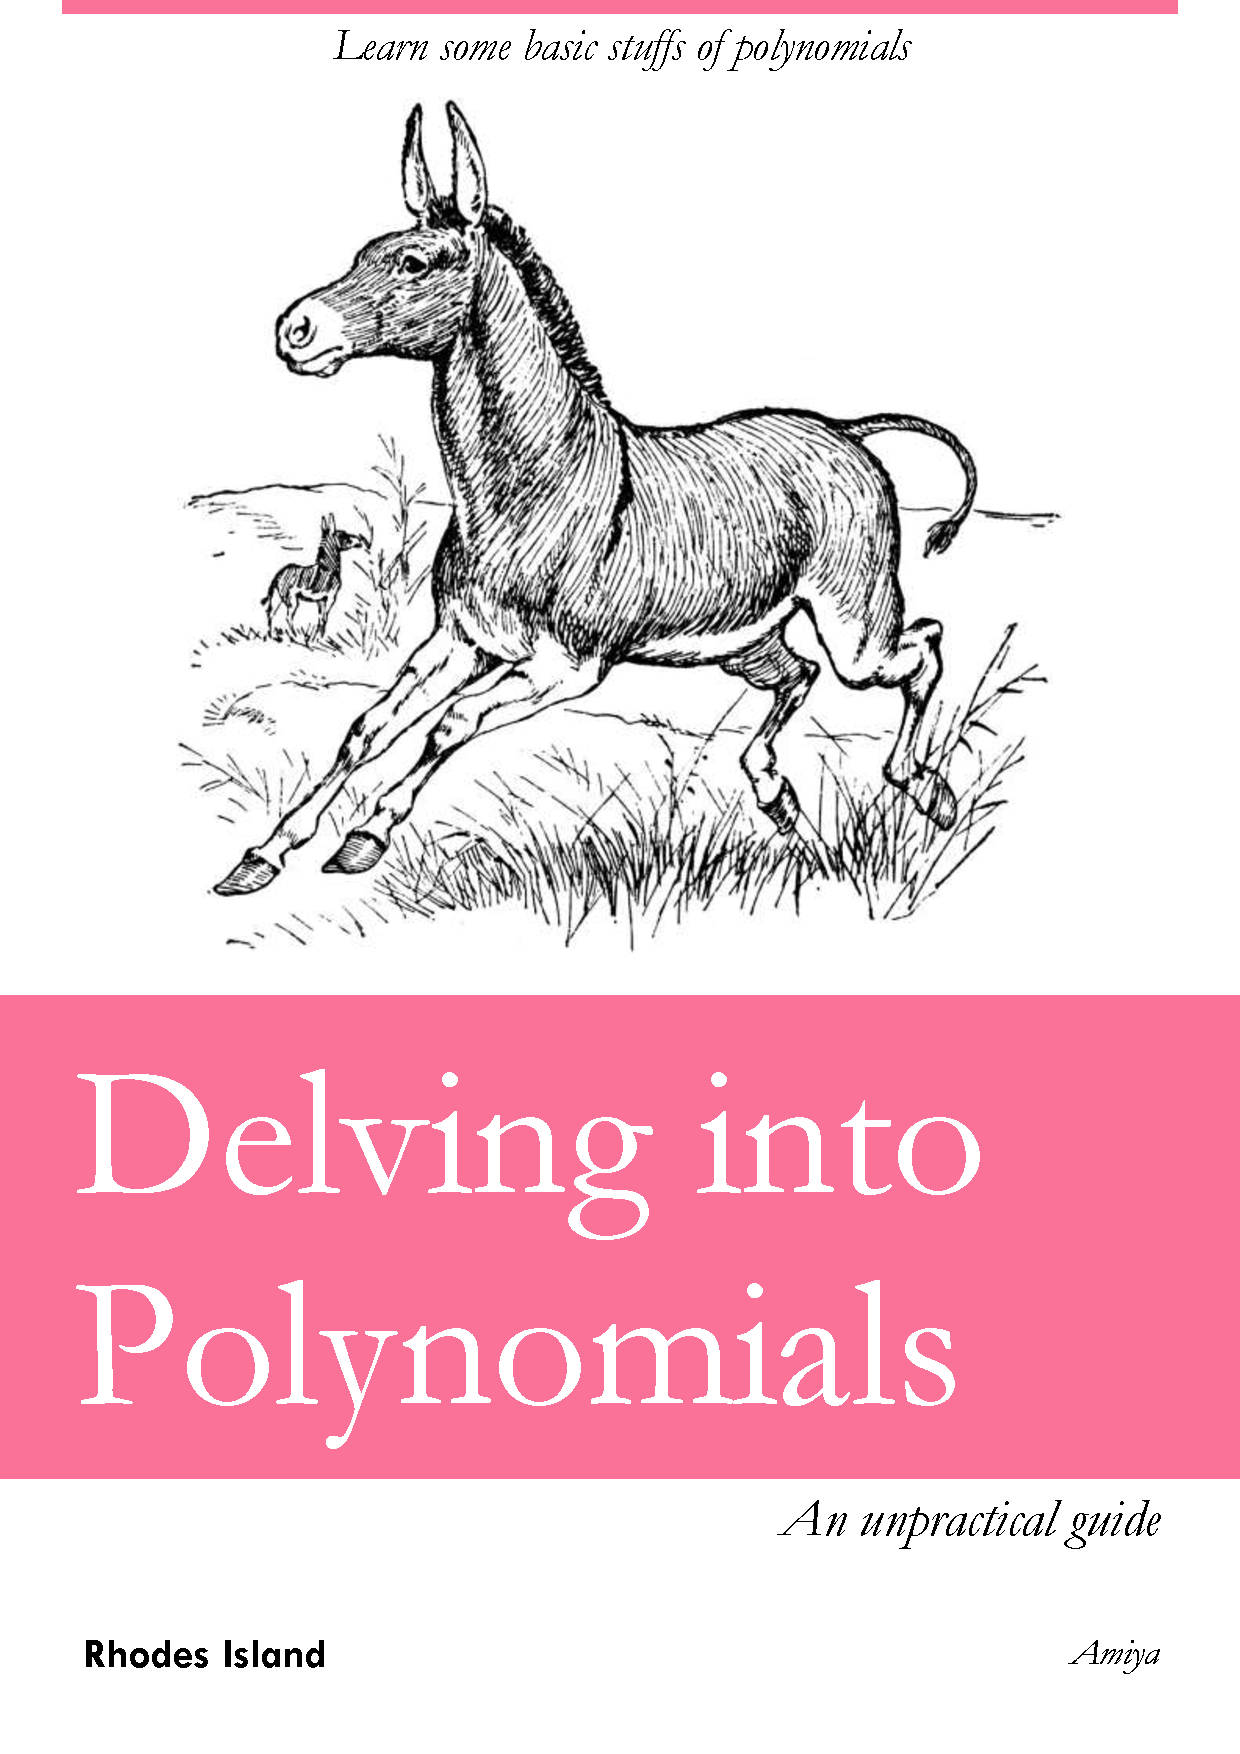
\includepdf{res/cover.pdf}
\ \
\clearpage

\title{}
\date{}
\author{}
\ctexset{today=old}
\pagestyle{plain}
\pagenumbering{roman}
\renewcommand{\contentsname}{Table of Contents}
\renewcommand{\abstractname}{Abstract}

\pagestyle{plain}
\thispagestyle{empty}
\tableofcontents

\newsection
\section*{License Notice}
% Use the following line to add the unnumbered section to the table of contents
\addcontentsline{toc}{section}{License Notice}

The source code of the work is licensed under \hyperref{https://unlicense.org/}{}{}{\textbf{the Unlicense}}:

\begin{quotation}
    \sffamily

    This is free and unencumbered software released into the public domain.

    Anyone is free to copy, modify, publish, use, compile, sell, or distribute this software, either in source code form or as a compiled binary, for any purpose, commercial or non-commercial, and by any means.

    In jurisdictions that recognize copyright laws, the author or authors of this software dedicate any and all copyright interest in the software to the public domain. We make this dedication for the benefit of the public at large and to the detriment of our heirs and successors. We intend this dedication to be an overt act of relinquishment in perpetuity of all present and future rights to this software under copyright law.

    THE SOFTWARE IS PROVIDED ``AS IS'', WITHOUT WARRANTY OF ANY KIND, EXPRESS OR IMPLIED, INCLUDING BUT NOT LIMITED TO THE WARRANTIES OF MERCHANTABILITY, FITNESS FOR A PARTICULAR PURPOSE AND NONINFRINGEMENT. IN NO EVENT SHALL THE AUTHORS BE LIABLE FOR ANY CLAIM, DAMAGES OR OTHER LIABILITY, WHETHER IN AN ACTION OF CONTRACT, TORT OR OTHERWISE, ARISING FROM, OUT OF OR IN CONNECTION WITH THE SOFTWARE OR THE USE OR OTHER DEALINGS IN THE SOFTWARE.

    For more information, please refer to
    \begin{center}
        \texttt{ \hyperref{https://unlicense.org}{}{}{<https://unlicense.org>} }
    \end{center}
\end{quotation}

The text is licensed under \hyperref{https://creativecommons.org/publicdomain/zero/1.0/}{}{}{\textbf{CC0}}. Here is the summary:

\begin{quotation}
    \sffamily

    \noindent \textbf{\large No Copyright}

    \vspace{1.5ex}

    The person who associated a work with this deed has \textbf{dedicated} the work to the public domain by waiving all of his or her rights to the work worldwide under copyright law, including all related and neighboring rights, to the extent allowed by law.

    You can copy, modify, distribute and perform the work, even for commercial purposes, all without asking permission. See \textbf{Other Information} below.

    \vspace{1.5ex}

    \noindent \textbf{\large Other Information}

    \vspace{1.5ex}

    \vspace{-\topsep}

    \begin{itemize}
        \item In no way are the patent or trademark rights of any person affected by CC0, nor are the rights that other persons may have in the work or in how the work is used, such as publicity or privacy rights.
        \item Unless expressly stated otherwise, the person who associated a work with this deed makes no warranties about the work, and disclaims liability for all uses of the work, to the fullest extent permitted by applicable law.
        \item When using or citing the work, you should not imply endorsement\myFN{In some jurisdictions, wrongfully implying that an author, publisher or anyone else endorses your use of a work may be unlawful.} by the author or the affirmer.
    \end{itemize}
\end{quotation}


\newsection
\section*{\Preface}
% Use the following line to add the unnumbered section to the table of contents
\addcontentsline{toc}{section}{\Preface}

本文是瞎写的. 作者给本文的另一个名字是 ``Re: ゼロ から 始める ポリノミアル の イントロダクション''. 不过想了想, 算了算了. 龙鸣日语, 不好意思直接说出来.

本文用尽可能朴素的语言讨论了多项式及其部分应用.

总是可以去这儿得到本文的最新版本:
\begin{align*}
     & \texttt{https://gitee.com/septsea/strange-book-zero}  \\
     & \texttt{https://github.com/septsea/strange-book-zero}
\end{align*}

读者可以自由地阅读、修改、再分发本文.

如果读者发现本文有什么地方不对, 那么读者就毫不犹豫地告诉作者. 当然, 任何意见与建议也是可以的.

(记得先看看最新版本改过来没有哟. 不过就算没看最新版本也没关系啦. 作者一定会处理读者的消息的! 嘿嘿.)

就先说到这里.

~\

\providecommand{\appendDate}{}
\renewcommand{\appendDate}[1]{\par \hfill {\itshape \sffamily #1}}

\begin{remark}
    总算写完 ``\Prerequisites '' 了. 作者写这玩意儿花了好久好久啊. 先发布再说吧.
    \appendDate{June 3, 2021}
\end{remark}

\begin{remark}
    忘记介绍域是什么东西了. 作者真是笨蛋啊.
    \appendDate{June 3, 2021}
\end{remark}

\begin{remark}
    前几日意识到, 作者不能又写得严谨, 又指望着中学生都能读懂. 不过本文业已成形, ``改'' 不如 ``重写''. 不过本文是开源的 (主要是无版权), 读者可以随意重写.
    \appendDate{June 17, 2021}
\end{remark}

\begin{remark}
    6 月 6 日, 作者在\hyperref{https://chaoli.club/index.php/6396}{}{}{这里}发了贴, 目的是让更多的人看到作者写的 \ding{200} 文. 作者得到了很多意见与建议. 今日, 作者写完了作者想写的东西. 作者维护本文就好. 作者觉得超理太棒了!
    \appendDate{June 20, 2021}
\end{remark}

\begin{remark}
    作者总算在改错了. 感谢超理读者 ``没啥好叫的'' 指出本文的一个错误! 然后作者自己发现了一堆印刷错误. 啊啦啊啦. 看多了视觉小说, 作者的大脑生锈了呢. 顺便一提, 看本文看累了的时候, 不妨看看小说哦! \hyperref{https://gitee.com/septsea/ss}{}{}{这里! 这里! I am sharing my copies of visual novels with my readers!}
    \appendDate{July 29, 2021}
\end{remark}


\newsection
\pagestyle{headings}
\setcounter{page}{1}
\pagenumbering{arabic}

\section*{Delving into Polynomials}
\addcontentsline{toc}{section}{Delving into Polynomials}
\markboth{Delving into Polynomials}{}

Out of boredom, I wrote the article.

    % This is used to occupy some space.
    {
        \vfill \itshape \sffamily \small
        \begin{center}
            \begin{tabular}{l}
                Gohan ni suru? Ofuro ni suru? Sore tomo\ellipsis \ wa ta shi? \\
                (Would you like dinner? Would you like a bath? Or\ellipsis \ would you like me?)
            \end{tabular}
        \end{center}
    }

\clearpage

\subsection*{\Prerequisites}
\addcontentsline{toc}{subsection}{\Prerequisites}
\markright{\Prerequisites}

读者将在本节熟悉一些记号与术语. 建议读者熟悉本节的内容后学习下节的内容.

在进入小节 ``\Sets '' 前, 让我们先回顾命题、复数与数学归纳法吧!

\begin{definition}
    能判断真假的话是命题 \term{proposition}. 正确的命题称为真命题; 错误的命题称为假命题. 当然, 命题也可以用 ``对'' ``错'' 形容.
\end{definition}

\begin{example}
    根据常识, ``日东升西落'' 是真命题. 类似地, ``月自身可发光'' 是假命题.

    ``这是什么?'' 不是命题, 因为它没有作出判断. 类似地, ``请保持安静'' 也不是命题, 因为它只是一个祈使句 \term{imperative sentence}. 不过, ``难道中国不强?'' 不但是命题, 它还是正确的, 因为这个反问 \term{rhetorical question} 作出了正确的判断.

    ``$x > 3$'' 不是命题, 因为它不可判断真假. 像这种话里有未知元, 且揭秘未知元前不可知此话之真伪的话是开句 \term{open sentence}.
\end{example}

我们会经常遇到 ``若 $p$, 则 $q$'' 的命题.

\begin{definition}
    设 ``若 $p$, 则 $q$'' 是真命题. 我们说, $p$ 是 $q$ 的充分条件 \term{sufficient condition}, $q$ 是 $p$ 的必要条件 \term{necessary condition}. 用符号写出来, 就是
    \begin{align*}
        p \Rightarrow q \quad \text{or} \quad q \Leftarrow p.
    \end{align*}
\end{definition}

\begin{example}
    ``若刚下过雨, 则地面潮湿'' 是对的. ``刚下过雨'' 是 ``充分的'': 根据常识可以知道这一点. ``地面潮湿'' 是 ``必要的'': 地面不潮湿, 那么不可能刚下过雨.
\end{example}

\begin{remark}
    我们会遇到形如 ``$\ell$ 的一个必要与充分条件是 $r$'' 的命题. 换个说法, 就是 ``$r$ 是 $\ell$ 的一个必要与充分条件''. 再分解一下, 就是 ``$r$ 是 $\ell$ 的一个必要条件'' 与 ``$r$ 是 $\ell$ 的一个充分条件'' 这二个命题. 根据定义, 这相当于 ``若 $\ell$, 则 $r$'' 与 ``若 $r$, 则 $\ell$'' 都是真命题. 也就是说, $\ell$ 跟 $r$ 是等价的 \term{equivalent}. 用符号写出来, 就是
    \begin{align*}
        p \Leftrightarrow q.
    \end{align*}

    证明 ``$\ell$ 的一个必要与充分条件是 $r$'' 时, 我们会把它分为必要性 \term{necessity} 与充分性 \term{sufficiency} 二个部分. 证明必要性, 就是证明 ``$r$ 是 $\ell$ 的一个必要条件'', 也就是证明 ``若 $\ell$, 则 $r$'' 是对的; 换句话说, 证明左边可以推出右边. 证明充分性, 就是证明 ``$r$ 是 $\ell$ 的一个充分条件'', 也就是证明 ``若 $r$, 则 $\ell$'' 是对的; 换句话说, 证明右边可以推出左边.
\end{remark}

命题就介绍到这里. 下面回顾复数基础.

\begin{definition}
    复数 \term{complex number} 是形如 $x + y \ii$ ($x$, $y$ 是实数) 的数.
\end{definition}

\begin{remark}
    可将 $x + y \ii$ 写为 $x + \ii y$.
\end{remark}

\begin{definition}
    设 $a,b,c,d$ 是实数. 则
    \begin{align*}
        a + b \ii = c + d \ii \iff a = c \text{ and } b = d.
    \end{align*}
\end{definition}

\begin{remark}
    我们把形如 $a+0 \ii$ 的复数写为 $a$, 并认为 $a+0 \ii$ 是实数. 反过来, $a$ 也可以认为是复数 $a + 0 \ii$.

    形如 $0 + b \ii$ 的复数可写为 $b \ii$. 按照习惯, $1\ii$ 可写为 $\ii$, 且 $-1\ii$ 可写为 $-\ii$.
\end{remark}

\begin{definition}
    复数的加、乘法定义为
    \begin{align*}
         & (a + b \ii) + (c + d \ii) = (a + c) + (b + d) \ii,   \\
         & (a + b \ii) (c + d \ii) = (ac - bd) + (ad + bc) \ii.
    \end{align*}
    由此可见, 二个复数的和 (或积) 还是复数.
\end{definition}

\begin{example}
    我们计算 $\ii$ 与自己的积:
    \begin{align*}
        \ii \cdot \ii = (0 + 1\ii) (0 + 1\ii) = (0 \cdot 0 - 1 \cdot 1) + (0 \cdot 1 + 1 \cdot 0) \ii = -1.
    \end{align*}
    简单地说, 就是
    \begin{align*}
        \ii \cdot \ii = \ii^2 = -1.
    \end{align*}
\end{example}

设 $z_1, z_2, z_3$ 是任意三个复数 (不必不同). 设 $z_1 = a + b \ii$.

\begin{proposition}
    复数的加法适合如下运算律:

    (i) 交换律: $z_1 + z_2 = z_2 + z_1$;

    (ii) 结合律: $(z_1 + z_2) + z_3 = z_1 + (z_2 + z_3)$;

    (iii) $0 + z_1 = z_1$;

    (iv) 存在复数 $w = (-a) + (-b) \ii$ 使 $w + z_1 = 0$.

    通常把适合 (iv) 的 $w$ 记为 $-z_1$, 且称之为 $z_1$ 的相反数.
\end{proposition}

\begin{remark}
    $(-a) + (-b) \ii$ 可写为 $-a-b \ii$.
\end{remark}

\begin{definition}
    复数的减法定义为
    \begin{align*}
        z_2 - z_1 = z_2 + (-z_1).
    \end{align*}
\end{definition}

\begin{proposition}
    复数的乘法适合如下运算律:

    (v) 交换律: $z_1 z_2 = z_2 z_1$;

    (vi) 结合律: $(z_1 z_2) z_3 = z_1 (z_2 z_3)$;

    (vii) $1 z_1 = z_1$;

    (viii) $(-1) z_1 = -z_1$;

    (ix) 若 $z_1 \neq 0$, 则存在复数 $v = \frac{a}{a^2 + b^2} + \frac{-b}{a^2 + b^2} \ii$ 使 $v z_1 = 1$.

    通常把适合 (ix) 的 $v$ 记为 $z_1^{-1}$, 且称之为 $z_1$ 的倒数.
\end{proposition}

\begin{definition}
    复数的除法定义为
    \begin{align*}
        \frac{z_2}{z_1} = z_2 z_1^{-1}.
    \end{align*}
\end{definition}

\begin{proposition}
    复数的加法与乘法还适合分配律:
    \begin{align*}
         & z_1 (z_2 + z_3) = z_1 z_2 + z_1 z_3, \\
         & (z_2 + z_3) z_1 = z_2 z_1 + z_3 z_1.
    \end{align*}
\end{proposition}

\begin{remark}
    $a$, $b\ii$, $c$, $d\ii$ 都可以看成是复数. 这样
    \begin{align*}
        (a + b \ii) (c + d \ii)
        = {} & (a + b \ii) c + (a + b \ii) (d \ii)  \\
        = {} & ac + b \ii c + a d \ii + b \ii d \ii \\
        = {} & ac + bc\ii + ad\ii + bd\ii^2         \\
        = {} & (ac + bd\ii^2) + (ad + bc)\ii        \\
        = {} & (ac - bd) + (ad + bc)\ii.
    \end{align*}
    也就是说, 我们不必死记复数的乘法规则: 只要用运算律与 $\ii^2 = -1$ 即可召唤它.
\end{remark}

\begin{definition}
    设 $a$, $b$ 是实数. $a + b\ii$ 的共轭 \term{conjugate} 是复数 $a - b\ii$. 复数 $z_1$ 的共轭可写为 $\overline{z_1}$.
\end{definition}

\begin{proposition}
    共轭适合如下性质:

    (x) $\overline{z_1} + z_1$ 与 $\ii \cdot (\overline{z_1} - z_1)$ 都是实数;

    (xi) $\overline{z_1 + z_2} = \overline{z_1} + \overline{z_2}$, $\overline{z_1 z_2} = \overline{z_1} \cdot \overline{z_2}$;

    (xii) $\overline{\overline{z_1}} = z_1$;

    (xiii) $\overline{z_1} z_1$ 是正数, 除非 $z_1 = 0$.
\end{proposition}

\begin{definition}
    $|z_1| = \sqrt{\overline{z_1} z_1}$ 称为 $z_1$ 的绝对值 \term{absolute value}.
\end{definition}

\begin{proposition}
    绝对值适合如下性质:
    \begin{align*}
        |z_1 z_2| = |z_1| |z_2|.
    \end{align*}
\end{proposition}

\begin{definition}
    设 $n$ 是整数. 若 $n=0$, 则说 $z_1^n = 1$. 若 $n \geq 1$, 则说 $z_1^n$ 是 $n$ 个 $z_1$ 的积. 若 $z_1 \neq 0$, 且 $n \leq -1$, 则说 $z_1^n$ 是 $\frac{1}{z_1^{-n}}$.

    $z_1^n$ 的一个名字是 $z_1$ 的 $n$ 次幂 \term{power}.
\end{definition}

\begin{proposition}
    设 $m,n$ 是非负整数. 幂适合如下性质:
    \begin{align*}
        z_1^m z_1^n = z_1^{m+n}, \quad (z_1^m)^n = z_1^{mn}, \quad (z_1 z_2)^m = z_1^m z_2^m.
    \end{align*}
    若 $z_1$ 与 $z_2$ 都不是 $0$, 则 $m,n$ 允许取全体整数.
\end{proposition}

复数就先回顾到这里. 下面回顾数学归纳法.

\begin{remark}
    数学归纳法 \term{mathematical induction} 是一种演绎推理.
\end{remark}

\begin{proposition}
    设 $P(n)$ 是跟整数 $n$ 相关的命题. 设 $P(n)$ 适合:

    (i) $P(n_0)$ 是正确的;

    (ii) 任取 $\ell \geq n_0$, 必有 ``若 $P(\ell)$ 是正确的, 则 $P(\ell + 1)$ 是正确的'' 成立.

    则任取不低于 $n_0$ 的整数 $n$, 必有 $P(n)$ 是正确的.
\end{proposition}

\begin{remark}
    可以这么理解数学归纳法. 假设有一排竖立的砖. 如果 (i) 第一块砖倒下, 且 (ii) 前一块砖倒下可引起后一块砖倒下, 那么所有的砖都可以倒下, 是吧? 由此也可以看出, (i) (ii) 缺一不可. 第一块砖不倒, 后面的砖怎么倒下呢?\myFN{当然, 也可以从第 $n$ 块砖开始倒下 ($n > 1$), 但这就照顾不到第一块了.} 如果前一块砖倒下时后一块砖不一定能倒下, 那么会在某块砖后开始倒不下去.
\end{remark}

\begin{example}
    我们试着用数学归纳法证明, 对任意正整数 $n$,
    \begin{align*}
        0 + 1 + \cdots + (n - 1) = \frac{n(n-1)}{2}. \tag*{$P(n) \colon$}
    \end{align*}

    既然想证明对任意正整数 $n$, $P(n)$ 都成立, 我们取 $n_0 = 1$. 然后验证 (i): 左边只有 $0$ 这一项, 右边是 $\frac{1 \cdot (1-1)}{2} = 0$. 所以 (i) 适合.

    再验证 (ii). (ii) 是说, 要由 $P(\ell)$ 推出 $P(\ell + 1)$. 所以, 假设
    \begin{align*}
        0 + 1 + \cdots + (\ell - 1) = \frac{\ell(\ell-1)}{2}, \quad \ell \geq n_0.
    \end{align*}
    因为
    \begin{align*}
        0 + 1 + \cdots + (\ell - 1) + \ell
        = {} & (0 + 1 + \cdots + (\ell - 1)) + \ell            \\
        = {} & \frac{\ell(\ell-1)}{2} + \ell \tag*{(IH)}       \\
        = {} & \frac{\ell(\ell-1)}{2} + \frac{\ell \cdot 2}{2} \\
        = {} & \frac{\ell(\ell+1)}{2}                          \\
        = {} & \frac{(\ell+1)((\ell+1) - 1)}{2},
    \end{align*}
    故我们由 $P(\ell)$ 推出了 $P(\ell + 1)$. 我们在哪儿用到了 $P(\ell)$ 呢? 我们在标了 (IH) 的那一行用了 $P(\ell)$. 这样的假设称为归纳假设 \term{induction hypothesis}.

    既然 (i) (ii) 都适合, 那么任取不低于 $n_0=1$ 的整数 $n$, $P(n)$ 都对.
\end{example}

我们用二个具体的例说明, (i) (ii) 缺一不可.

\begin{example}
    我们 ``证明'', 对任意正整数 $n$,
    \begin{align*}
        0 + 1 + \cdots + (n - 1) = \frac{n(n-1)}{2} + 1. \tag*{$P^{\prime}(n) \colon$}
    \end{align*}
    这里, $n_0$ 自然取 $1$.

    (i) 不适合: 显然 $n=1$ 时, 左侧是 $0$ 而右侧是 $1$. 再看 (ii). 假设
    \begin{align*}
        0 + 1 + \cdots + (\ell - 1) = \frac{\ell(\ell-1)}{2} + 1, \quad \ell \geq n_0.
    \end{align*}
    由于
    \begin{align*}
        0 + 1 + \cdots + (\ell - 1) + \ell
        = {} & (0 + 1 + \cdots + (\ell - 1)) + \ell                \\
        = {} & \frac{\ell(\ell-1)}{2} + 1 + \ell \tag*{(``IH'')}   \\
        = {} & \frac{\ell(\ell-1)}{2} + \frac{\ell \cdot 2}{2} + 1 \\
        = {} & \frac{\ell(\ell+1)}{2} + 1                          \\
        = {} & \frac{(\ell+1)((\ell+1) - 1)}{2} + 1,
    \end{align*}
    故我们由 $P^{\prime}(\ell)$ ``推出''了 $P^{\prime}(\ell + 1)$. 我们也在 (``IH'') 处用到了 ``归纳假设''. 那么 $P^{\prime}(n)$ 就是正确的吗? 当然不是! 前面我们知道,
    \begin{align*}
        0 + 1 + \cdots + (n - 1) = \frac{n(n-1)}{2},
    \end{align*}
    也就是说, $P^{\prime}(n)$ 的右侧的 ``${} + 1$'' 使其错误. 当然, 一般我们很少会犯这样的错误: 毕竟, 一开始就不对的东西就不用看下去了.
\end{example}

\begin{example}
    % cSpell: disable-next-line
    不同的老婆\myFN{一般地, 二次元人会称动画、漫画、游戏、小说中自己喜爱的女性角色为老婆 \term{waifu}. 一个二次元人可以有不止一个老婆.}有着不同的发色. 但是, 我们用数学归纳法却可以 ``证明'', 任意的 $n$ ($n \geq 1$) 个老婆有着相同的发色! 称这个命题为 $Q(n)$. 这里, $n_0$ 自然取 $1$.

    (i) 当 $n=n_0=1$ 时, 一个老婆自然只有一种发色. 这个时候, 命题是正确的!

    (ii) 假设任意的 $\ell$ ($\ell \geq n_0$) 个老婆有着相同的发色! 随意取 $\ell + 1$ 个老婆. 根据假设, 老婆 $1$, $2$, $\cdots$, $\ell$ 有着相同的发色, 且老婆 $2$, $\cdots$, $\ell$, $\ell+1$ 有着相同的发色. 这二组中都有 $2$, $\cdots$, $\ell$ 这 $\ell-1$ 个老婆, 所以老婆 $1$, $2$, $\cdots$, $\ell$, $\ell+1$ 有着相同的发色!

    根据 (i) (ii), 命题成立.

    可是这对吗? 不对. 问题出在 (ii). 如果说, 任意二个老婆有着相同的发色, 那任意三个老婆也有着相同的发色. 这没问题. 可是, 由 $Q(1)$ 推不出 $Q(2)$: 老婆 $1$ 与老婆 $2$ 根本就不重叠呀! (ii) 要求任取 $\ell \geq n_0$, 必有 $Q(\ell)$ 推出 $Q(\ell+1)$. 而 $\ell = 1$ 时, (ii) 不对, 因此不能推出 $Q(n)$ 对任意正整数都对.
\end{example}

下面是数学归纳法的一个变体.

\begin{proposition}
    设 $P(n)$ 是跟整数 $n$ 相关的命题. 设 $P(n)$ 适合:

    (i) $P(n_0)$ 是正确的;

    (ii)$^{\prime}$ 任取 $\ell \geq n_0$, 必有 ``若 $\ell - n_0 + 1$ 个命题 $P(n_0)$, $P(n_0 + 1)$, $\cdots$, $P(\ell)$ 都是正确的, 则 $P(\ell + 1)$ 是正确的'' 成立.

    则任取不低于 $n_0$ 的整数 $n$, 必有 $P(n)$ 是正确的.
\end{proposition}

\begin{remark}
    可以由下面的推理看出, 上面的数学归纳法变体是正确的.

    作命题 $Q(n)$ ($n \geq n_0$) 为 ``$n - n_0 + 1$ 个命题 $P(n_0)$, $P(n_0 + 1)$, $\cdots$, $P(n)$ 都是正确的''.

    (i) $P(n_0)$ 是正确的, 所以 $n_0 - n_0 + 1$ 个命题 $P(n_0)$ 是正确的, 也就是 $Q(n_0)$ 是正确的.

    (ii) 任取 $\ell \geq n_0$. 假设 $Q(\ell)$ 是正确的, 也就是假设 $\ell - n_0 + 1$ 个命题 $P(n_0)$, $P(n_0 + 1)$, $\cdots$, $P(\ell)$ 都是正确的. 由 (ii)$^{\prime}$, $P(\ell + 1)$ 是正确的. 所以, $\ell + 1 - n_0 + 1$ 个命题 $P(n_0)$, $P(n_0 + 1)$, $\cdots$, $P(\ell)$, $P(\ell + 1)$ 都是正确的. 换句话说, $Q(\ell + 1)$ 是正确的.

    由数学归纳法可知, 任取不低于 $n_0$ 的整数 $n$, 必有 $Q(n)$ 是正确的. 所以, $P(n)$ 是正确的.

    另一方面, 这个变体的条件 (ii)$^{\prime}$ 比数学归纳法的 (ii) 强, 所以若变体正确, 数学归纳法也正确. 也就是说, 数学归纳法与其变体是等价的.

    以后, ``数学归纳法'' 既可以指老的数学归纳法 (由 $P(\ell)$ 推 $P(\ell+1)$), 也可以指变体 (由 $P(n_0)$, $P(n_0 + 1)$, $\cdots$, $P(\ell)$ 推 $P(\ell+1)$).
\end{remark}

知识就回顾到这里. 开始进入集的世界吧!

\subsubsection*{\Sets}

\begin{definition}
    集 \term{set} 是具有某种特定性质的对象汇集而成的一个整体, 其对象称为元 \term{element}.
\end{definition}

\begin{definition}
    无元的集是空集 \term{empty set}.
\end{definition}

\begin{remark}
    一般用小写字母表示元, 大写字母表示集.
\end{remark}

\begin{definition}
    一般地, 若集 $A$ 由元 $a$, $b$, $c$, $\cdots$ 作成, 我们写
    \begin{align*}
        A = \{\, a,b,c,\cdots \,\}.
    \end{align*}
    还有一种记号. 设集 $A$ 是由具有某种性质 $p$ 的对象汇集而成, 则记
    \begin{align*}
        A = \{\, x \mid x \text{ possesses the property } p \,\}.
    \end{align*}
\end{definition}

\begin{definition}
    若 $a$ 是集 $A$ 的元, 则写 $a \in A$ 或 $A \ni a$, 说 $a$ 属于 \term{to belong to} $A$ 或 $A$ 包含 \term{to contain} $a$. 若 $a$ 不是集 $A$ 的元, 则写 $a \notin A$ 或 $A \not\ni a$, 说 $a$ 不属于 $A$ 或 $A$ 不包含 $a$.
\end{definition}

\begin{example}
    % cSpell: disable-next-line
    全体整数作成的集用 $\ZZ$ \term{Zahl}\myFN{A German word which means \textit{number}.} 表示. 它可以写为
    \begin{align*}
        \ZZ = \{\, 0,1,-1,2,-2,\cdots,n,-n,\cdots \,\}.
    \end{align*}
\end{example}

\begin{example}
    全体非负整数作成的集用 $\NN$ \term{natural} 表示. 它可以写为
    \begin{align*}
        \NN = \{\, x \mid x \in \ZZ \text{ and } x \geq 0 \,\}.
    \end{align*}
    为了方便, 也可以写为
    \begin{align*}
        \NN = \{\, x \in \ZZ \mid x \geq 0 \,\}.
    \end{align*}
\end{example}

\begin{definition}
    若任取 $a \in A$, 都有 $a \in B$, 则写 $A \subset B$ 或 $B \supset A$, 说 $A$ 是 $B$ 的子集 \term{subset} 或 $B$ 是 $A$ 的超集 \term{superset}. 假如有一个 $b \in B$ 不是 $A$ 的元, 可以用 ``真'' \term{proper} 形容之.
\end{definition}

\begin{example}
    空集是任意集的子集. 空集是任意不空的集的真子集.
\end{example}

\begin{example}
    全体有理数作成的集用 $\QQ$ \term{quotient} 表示. 因为整数是有理数, 所以 $\ZZ \subset \QQ$. 因为有理数 $\frac12$ 不是整数, 我们说 $\ZZ$ 是 $\QQ$ 的真子集.
\end{example}

\begin{definition}
    全体实数作成的集用 $\RR$ \term{real} 表示.
\end{definition}

\begin{definition}
    全体复数作成的集用 $\CC$ \term{complex} 表示. 不难看出,
    \begin{align*}
        \NN \subset \ZZ \subset \QQ \subset \RR \subset \CC.
    \end{align*}
\end{definition}

\begin{definition}
    $\FF$ \term{field} 可表示 $\QQ$, $\RR$, $\CC$ 的任意一个. 不难看出, $\FF$ 适合这几条:

    (i) $0 \in \FF$, $1 \in \FF$, $0 \neq 1$;

    (ii) 任取 $x,y \in \FF$ ($y \neq 0$), 必有 $x-y, \frac{x}{y} \in \FF$.

    后面会见到稍详细的论述.
\end{definition}

\begin{definition}
    设 $\mathbb{L}$ 是 $\CC$, $\RR$, $\QQ$, $\ZZ$, $\NN$, $\FF$ 的任意一个. $\mathbb{L}^{\ast}$ 表示 $\mathbb{L}$ 去掉 $0$ 后得到的集. 不难看出, $\mathbb{L}$ 是 $\mathbb{L}^{\ast}$ 的真超集.
\end{definition}

\begin{definition}
    若集 $A$ 与 $B$ 包含的元完全一样, 则 $A$ 与 $B$ 是同一集. 我们说 $A$ 等于 $B$, 写 $A = B$. 显然
    \begin{align*}
        A = B \iff A \subset B \text{ and } B \subset A.
    \end{align*}
\end{definition}

\begin{definition}
    集 $A$ 与 $B$ 的交 \term{intersection} 是集
    \begin{align*}
        A \cap B = \{\, x \mid x \in A \text{ and } x \in B \,\}.
    \end{align*}
    也就是说, $A \cap B$ 恰由 $A$ 与 $B$ 的公共元作成.

    集 $A$ 与 $B$ 的并 \term{union} 是集
    \begin{align*}
        A \cup B = \{\, x \mid x \in A \text{ or } x \in B \,\}.
    \end{align*}
    也就是说, $A \cup B$ 恰包含 $A$ 与 $B$ 的全部元.

    类似地, 可定义多个集的交与并.
\end{definition}

\begin{definition}
    设 $A$, $B$ 是集. 定义
    \begin{align*}
        A \times B = \{\, (a,b) \mid a \in A, \ b \in B  \,\}.
    \end{align*}
    $A \times A$ 可简写为 $A^2$. 类似地,
    \begin{align*}
        A \times B \times C = \{\, (a,b,c) \mid a \in A, \ b \in B, \ c \in C  \,\}, \quad A^3 = A \times A \times A.
    \end{align*}
\end{definition}

\begin{example}
    设 $A = \{\, 1,2 \,\}$, $B = \{\, 3,4,5 \,\}$. 则
    \begin{align*}
        A \times B = \{\, (1,3),(1,4),(1,5),(2,3),(2,4),(2,5) \,\}.
    \end{align*}
    而
    \begin{align*}
        B \times A = \{\, (3,1),(3,2),(4,1),(4,2),(5,1),(5,2) \,\}.
    \end{align*}
\end{example}

\begin{remark}
    一般地, $A \times B \neq B \times A$. 假如 $A$, $B$ 各自有 $m$, $n$ 个元, 利用一点计数知识可以看出, $A \times B$ 有 $mn$ 个元.
\end{remark}

\subsubsection*{\Functions}

\begin{definition}
    假如通过一个法则 $f$, 使任取 $a \in A$, 都能得到唯一的 $b \in B$, 则说这个法则 $f$ 是集 $A$ 到集 $B$ 的一个函数 \term{function}. 元 $b$ 是元 $a$ 在函数 $f$ 下的象 \term{image}. 元 $a$ 是元 $b$ 在 $f$ 下的一个原象 \term{inverse image}. 这个关系可以写为
    \begin{align*}
         & A \to B,  \tag*{$f$:} \\
         & a \mapsto b = f(a).
    \end{align*}
    称 $A$ 是定义域 \term{domain}, $B$ 是陪域\myFN{不要混淆陪域与象集 (\textit{image}, \textit{range}). $f$ 的象集是
        \begin{align*}
            \mathrm{Im} \, f = \{\, b \in B \mid b = f(a), \, a \in A \,\}.
        \end{align*}
        这就是中学数学里的 ``值域''.
        % cSpell: disable-next-line
    } \term{codomain}.
\end{definition}

\begin{example}
    可以把 $\RR^2$ 看作平面上的点集.
    \begin{align*}
         & \RR^2 \to \RR,  \tag*{$f$:}  \\
         & (x,y) \mapsto \sqrt{x^2+y^2}
    \end{align*}
    是函数: 它表示点 $(x,y)$ 到点 $(0,0)$ 的距离.
\end{example}

\begin{example}
    设
    \begin{align*}
         & A = \{\, \text{dinner}, \text{bath}, \text{me} \,\}, \quad B = \{\, 0,1 \,\}.
    \end{align*}

    法则
    \begin{align*}
         & \text{dinner} \mapsto 0, \quad \text{bath} \mapsto 1 \tag*{$f_1$:}
    \end{align*}
    不是 $A$ 到 $B$ 的函数, 因为它没有为 $A$ 的元 $\text{me}$ 规定象. 但是, 如果记 $A_1 = \{\, \text{dinner}, \text{bath} \,\}$, 这个 $f_1$ 可以是 $A_1$ 到 $B$ 的函数.

    法则
    \begin{align*}
         & \text{dinner} \mapsto 0, \tag*{$f_2$:}          \\
         & \text{bath} \mapsto 1,                          \\
         & \text{me} \mapsto b \quad \text{where } b^2 = b
    \end{align*}
    不是 $A$ 到 $B$ 的函数, 因为它给 $A$ 的元 $\text{me}$ 规定的象不唯一.

    法则
    \begin{align*}
         & \text{dinner} \mapsto 0, \quad
        \text{bath} \mapsto 1, \quad
        \text{me} \mapsto -1 \tag*{$f_3$:}
    \end{align*}
    不是 $A$ 到 $B$ 的函数, 因为它给 $A$ 的元 $\text{me}$ 规定的象不是 $B$ 的元. 但是, 如果记 $B_1 = \{\, -1,0,1 \,\}$, 这个 $f_3$ 可以是 $A$ 到 $B_1$ 的函数.
\end{example}

\begin{definition}
    设 $f_1$ 与 $f_2$ 都是 $A$ 到 $B$ 的函数. 若任取 $a \in A$, 必有 $f_1 (a) = f_2 (a)$, 则说这二个函数相等, 写为 $f_1 = f_2$.
\end{definition}

\begin{example}
    设 $A \subset \CC$, 且 $A$ 非空. 定义二个 $A$ 到 $\CC$ 的函数: $f_1 (x) = x^2$, $f_2 (x) = |x|^2$. 如果 $A = \RR$, 那么 $f_1 = f_2$. 可是, 若 $A = \CC$, $f_1$ 与 $f_2$ 不相等.
\end{example}

\begin{example}
    设 $A$ 是全体正实数作成的集. 定义二个 $A$ 到 $\RR$ 的函数: $f_1 (x) = \frac16 \log_{2} {x^3}$, $f_2 (x) = \log_{4} {x}$. 知道对数的读者可以看出, $f_1$ 与 $f_2$ 有着相同的对应法则, 故 $f_1 = f_2$. 因为 $f_2$ 是对数函数 \term{logarithmic function}, 所以 $f_1$ 也是.
\end{example}

\begin{remark}
    在上下文清楚的情况下, 可以单说函数的对应法则. 比如, 中学数学课说 ``二次函数 $f(x) = x^2 + x - 1$'' 时, 定义域与陪域默认都是 $\RR$. 中学的函数一般都是实数的子集到实数的子集的函数. 所谓 ``自然定义域'' 是指 (在一定范围内) 一切使对应法则有意义的元构成的集. 比如, 在中学, 我们说 $\frac{1}{x}$ 的自然定义域是 $\RR^{\ast}$, $\sqrt{x}$ 的自然定义域是一切非负实数. 在研究复变函数时, 我们说 $\frac{1}{z}$ 的自然定义域是 $\CC^{\ast}$. 如果不明确函数的定义域, 我们会根据上下文作出自然定义域作为它的定义域.
\end{remark}

\begin{definition}
    $A$ 到 $A$ 的函数是 $A$ 的变换 \term{transform}. 换句话说, 变换是定义域跟陪域一样的函数.
\end{definition}

\subsubsection*{\BinaryFunctions}

\begin{definition}
    $A^2$ 到 $A$ 的函数称为 $A$ 的二元运算 \term{binary functions}.
\end{definition}

\begin{example}
    设 $f(x,y) = x-y$. 这个 $f$ 是 $\ZZ$ 的二元运算; 但是, 它不是 $\NN$ 的二元运算.
\end{example}

\begin{remark}
    设 $\circ$ 是 $A$ 的二元运算. 代替 $\circ (x,y)$, 我们写 $x \circ y$. 一般地, 若表示这个二元运算的符号不是字母, 我们就把这个符号写在二个元的中间.
\end{remark}

\begin{definition}
    设 $T(A)$ 是全部 $A$ 的变换作成的集. 设 $f,g$ 是 $A$ 的变换. 任取 $a \in A$, 当然有 $b = f(a) \in A$. 所以, $g(b) = g(f(a))$ 也是 $A$ 的元. 当然, 这个 $g(f(a))$ 也是唯一确定的. 这样, 我们说, $f$ 与 $g$ 的复合 \term{composition} $g \circ f$ 是
    \begin{align*}
         & A \to A, \tag*{$g \circ f \colon$} \\
         & a \mapsto g(f(a)).
    \end{align*}
    所以, 复合是 $T(A)$ 的二元运算:
    \begin{align*}
         & T(A) \times T(A) \to T(A), \tag*{$\circ \colon$} \\
         & (g,f) \mapsto g \circ f.
    \end{align*}
\end{definition}

\begin{remark}
    设 $A$ 有有限多个元. 此时, 可排出 $A$ 的元:
    \begin{align*}
        A = \{\, a_1, a_2, \cdots, a_n \,\}.
    \end{align*}
    设 $f$ 是 $A^2$ 到 $B$ 的函数. 则任给整数 $i,j$, $1 \leq i,j \leq n$, 记
    \begin{align*}
        f(a_i, a_j) = b_{i,j} \in B.
    \end{align*}
    可以用这样的表描述此函数:
    \begin{align*}
        \arraycolsep=0.25cm
        \begin{array}{c|cccc}
            \      & a_1     & a_2     & \cdots & a_n     \\ \hline
            a_1    & b_{1,1} & b_{1,2} & \cdots & b_{1,n} \\
            a_2    & b_{2,1} & b_{2,2} & \cdots & b_{2,n} \\
            \vdots & \vdots  & \vdots  & \ddots & \vdots  \\
            a_n    & b_{n,1} & b_{n,2} & \cdots & b_{n,n} \\
        \end{array}
    \end{align*}
    有的时候, 为了强调函数名, 可在左上角书其名:
    \begin{align*}
        \arraycolsep=0.25cm
        \begin{array}{c|cccc}
            f      & a_1     & a_2     & \cdots & a_n     \\ \hline
            a_1    & b_{1,1} & b_{1,2} & \cdots & b_{1,n} \\
            a_2    & b_{2,1} & b_{2,2} & \cdots & b_{2,n} \\
            \vdots & \vdots  & \vdots  & \ddots & \vdots  \\
            a_n    & b_{n,1} & b_{n,2} & \cdots & b_{n,n} \\
        \end{array}
    \end{align*}
    这种表示函数的方式是方便的. 如果这些 $b_{i,j}$ 都是 $A$ 的元, 就说这张表是 $A$ 的运算表.
\end{remark}

\begin{example}
    设 $T = \{\, 0,1,-1 \,\}$, $\circ (x,y) = xy$. 不难看出, $\circ$ 确实是 $T$ 的二元运算. 它的运算表如下:
    \begin{align*}
        \arraycolsep=0.25cm
        \begin{array}{c|ccc}
            \  & 0 & 1  & -1 \\ \hline
            0  & 0 & 0  & 0  \\
            1  & 0 & 1  & -1 \\
            -1 & 0 & -1 & 1  \\
        \end{array}
    \end{align*}
\end{example}

\begin{example}
    设 $\FF_{\mathrm{nu}}$ 是将 $\FF$ 去掉 $0$, $1$ 后得到的集\myFN{这个 $\FF_{\mathrm{nu}}$ 只是临时记号: $\mathrm{nu}$ 表示 \textit{nil}, \textit{unity}.}. 看下列 $6$ 个法则:
    \begin{align*}
         & x \mapsto x; \tag*{$f_0 \colon$}               \\
         & x \mapsto 1-x; \tag*{$f_1 \colon$}             \\
         & x \mapsto \frac{1}{x}; \tag*{$f_2 \colon$}     \\
         & x \mapsto 1-\frac{1}{1-x}; \tag*{$f_3 \colon$} \\
         & x \mapsto 1-\frac{1}{x}; \tag*{$f_4 \colon$}   \\
         & x \mapsto \frac{1}{1-x}. \tag*{$f_5 \colon$}
    \end{align*}
    记 $S_6 = \{\, f_0,f_1,f_2,f_3,f_4,f_5 \,\}$. 可以验证, $S_6 \subset T(\FF_{\mathrm{nu}})$.

    进一步地, $36$ 次复合告诉我们, 任取 $f,g \in S_6$, 必有 $g \circ f \in S_6$. 可以验证, 这是 $S_6$ 的 (复合) 运算表:
    \begin{align*}
        \arraycolsep=0.25cm
        \begin{array}{c|cccccc}
            \     & f_{0} & f_{1} & f_{2} & f_{3} & f_{4} & f_{5} \\ \hline
            f_{0} & f_{0} & f_{1} & f_{2} & f_{3} & f_{4} & f_{5} \\
            f_{1} & f_{1} & f_{0} & f_{4} & f_{5} & f_{2} & f_{3} \\
            f_{2} & f_{2} & f_{5} & f_{0} & f_{4} & f_{3} & f_{1} \\
            f_{3} & f_{3} & f_{4} & f_{5} & f_{0} & f_{1} & f_{2} \\
            f_{4} & f_{4} & f_{3} & f_{1} & f_{2} & f_{5} & f_{0} \\
            f_{5} & f_{5} & f_{2} & f_{3} & f_{1} & f_{0} & f_{4} \\
        \end{array}
    \end{align*}

    我们在本节会经常用 $S_6$ 举例.
\end{example}

\begin{definition}
    设 $\circ$ 是 $A$ 的二元运算. 若任取 $x,y,z \in A$, 必有
    \begin{align*}
        (x \circ y) \circ z = x \circ (y \circ z),
    \end{align*}
    则说 $f$ 适合结合律 \term{associativity}. 此时, $(x \circ y) \circ z$ 或 $x \circ (y \circ z)$ 可简写为 $x \circ y \circ z$.
\end{definition}

\begin{example}
    $\ZZ$ 的加法当然适合结合律. 可是, 它的减法不适合结合律.
\end{example}

\begin{remark}
    变换的复合适合结合律. 确切地, 设 $f,g,h$ 都是 $A$ 的变换. 任取 $a \in A$, 则
    \begin{align*}
         & (h \circ (g \circ f))(a) = h((g \circ f)(a)) = h(g(f(a))), \\
         & ((h \circ g) \circ f)(a) = (h \circ g)(f(a)) = h(g(f(a))).
    \end{align*}
    也就是说,
    \begin{align*}
        h \circ (g \circ f) = (h \circ g) \circ f.
    \end{align*}
\end{remark}

\begin{example}
    $S_6$ 的复合当然适合结合律.
\end{example}

\begin{definition}
    设 $\circ$ 是 $A$ 的二元运算. 若任取 $x,y \in A$, 必有
    \begin{align*}
        x \circ y = y \circ x,
    \end{align*}
    则说 $\circ$ 适合交换律 \term{commutativity}.
\end{definition}

\begin{example}
    $\FF^{\ast}$ 的乘法当然适合交换律. 可是, 它的除法不适合交换律.
\end{example}

\begin{example}
    $S_6$ 的复合不适合交换律, 因为 $f_1 \circ f_2 = f_4$, 而 $f_2 \circ f_1 = f_5$, 二者不相等.
\end{example}

\begin{remark}
    在本文里, $\cdot$ 运算的优先级高于 $+$ 运算. 所以, $a \cdot b + c$ 的意思就是
    \begin{align*}
        (a \cdot b) + c,
    \end{align*}
    而不是
    \begin{align*}
        a \cdot (b + c).
    \end{align*}
\end{remark}

\begin{definition}
    设 $+$, $\cdot$ 是 $A$ 的二个二元运算. 若任取 $x,y,z \in A$, 必有
    \begin{align*}
         & x \cdot (y + z) = x \cdot y + x \cdot z, \tag*{(LD)}
    \end{align*}
    则说 $+$ 与 $\cdot$ 适合左 ($\cdot$) 分配律\myFN{在不引起歧义时, 括号里的内容可省略. 或者这么说: 当我们说 $+$, $\cdot$ 适合分配律时, 我们不会理解为 $x + (y \cdot z) = (x + y) \cdot (x + z)$. 但有意思的事儿是, 如果把 $+$ 理解为并, $\cdot$ 理解为交, $x$, $y$, $z$ 理解为集, 那这个式是对的. 当然, $x \cdot (y + z) = x \cdot y + x \cdot z$ 也是对的.} \term{left distributivity}. 类似地, 若
    \begin{align*}
         & (y + z) \cdot x = y \cdot x + z \cdot x, \tag*{(RD)}
    \end{align*}
    则说 $+$ 与 $\cdot$ 适合右 ($\cdot$) 分配律 \term{right distributivity}. 说既适合 LD 也适合 RD 的 $+$ 与 $\cdot$ 适合 ($\cdot$) 分配律 \term{distributivity}. 显然, 若 $\cdot$ 适合交换律, 则 LD 与 RD 等价.
\end{definition}

\begin{example}
    $\FF$ 的加法与乘法适合分配律. 当然, 减法与乘法也适合分配律:
    \begin{align*}
        x(y-z) = xy - xz = yx - zx = (y-z)x.
    \end{align*}
    甚至, 在正实数里, 加法与除法适合右分配律:
    \begin{align*}
        \frac{y+z}{x} = \frac{y}{x} + \frac{z}{x}.
    \end{align*}
\end{example}

\begin{definition}
    设 $\circ$ 是 $A$ 的二元运算. 若任取 $x,y,z \in A$, 必有
    \begin{align*}
         & x \circ y = x \circ z \implies y = z, \tag*{(LC)}
    \end{align*}
    则说 $\circ$ 适合左消去律 \term{left cancellation property}. 类似地, 若
    \begin{align*}
         & x \circ z = y \circ z \implies x = y, \tag*{(RC)}
    \end{align*}
    则说 $\circ$ 适合右消去律 \term{right cancellation property}. 说既适合 LC 也适合 RC 的 $\circ$ 适合消去律 \term{cancellation property}. 显然, 若 $\circ$ 适合交换律, 则 LC 与 RC 等价.
\end{definition}

\begin{example}
    显然, $\NN$ 的乘法不适合消去律, 但 $\NN^{\ast}$ 的乘法适合消去律\myFN{后面提到整环时, 我们会稍微修改一下消去律的描述.}.
\end{example}

\begin{example}
    考虑 $x \circ y = x^3 + y^2$. 若把 $\circ$ 视为 $\NN$ 的二元运算, 那么它适合消去律. 若把 $\circ$ 视为 $\QQ$ 的二元运算, 那么它适合右消去律. 若把 $\circ$ 视为 $\CC$ 的二元运算, 那么它不适合任意一个消去律.
\end{example}

\begin{example}
    一般地, 当 $A$ 至少有二个元时, $\circ$ (在 $T(A)$ 里) 不适合消去律. 设 $a,b \in A$, $a \neq b$. 考虑下面 $4$ 个变换:
    \begin{align*}
         & a \mapsto a, \quad b \mapsto b, \quad x \mapsto x \text{ where $x \neq a,b$}; \tag*{$g_0 \colon$} \\
         & a \mapsto a, \quad b \mapsto a, \quad x \mapsto x \text{ where $x \neq a,b$}; \tag*{$g_1 \colon$} \\
         & a \mapsto b, \quad b \mapsto b, \quad x \mapsto x \text{ where $x \neq a,b$}; \tag*{$g_2 \colon$} \\
         & a \mapsto b, \quad b \mapsto a, \quad x \mapsto x \text{ where $x \neq a,b$}. \tag*{$g_3 \colon$}
    \end{align*}
    可以验证,
    \begin{align*}
        g_3 \circ g_1 = g_2 \circ g_1 = g_2 \circ g_3 = g_2.
    \end{align*}
    由此可以看出, $\circ$ 不适合任意一个消去律.
\end{example}

\begin{example}
    我们看 $\circ$ 在 $S_6$ 里是否适合消去律. 取 $f,g,h \in S_6$. 由表易知, 当 $g \neq h$ 时, $f \circ g \neq f \circ h$ (横着看运算表), 且 $g \circ f \neq h \circ f$ (竖着看运算表). 这说明, $\circ$ 在 $T(\FF_{\mathrm{nu}})$ 的子集 $S_6$ 里适合消去律.
\end{example}

\begin{definition}
    设 $\circ$ 是 $A$ 的二元运算. 若存在 $e \in A$, 使若任取 $x \in A$, 必有
    \begin{align*}
        e \circ x = x \circ e = x,
    \end{align*}
    则说 $e$ 是 $A$ 的 (关于运算 $\circ$ 的) 幺元 \term{identity}. 如果 $e^{\prime}$ 也是幺元, 则
    \begin{align*}
        e = e \circ e^{\prime} = e^{\prime}.
    \end{align*}
\end{definition}

\begin{example}
    $\FF$ 的加法的幺元是 $0$, 且其乘法的幺元是 $1$.
\end{example}

\begin{example}
    不难看出, 这个变换是 $T(A)$ 的幺元:
    \begin{align*}
         & A \to A,  \tag*{$\iota$:} \\
         & a \mapsto a.
    \end{align*}
    它也有个一般点的名字: 恒等变换 \term{identity transform}.

    在 $S_6$ 里, $f_0$ 就是这里的 $\iota$.
\end{example}

\begin{definition}
    设 $\circ$ 是 $A$ 的二元运算. 设 $e$ 是 $A$ 的幺元. 设 $x \in A$. 若存在 $y \in A$, 使
    \begin{align*}
        y \circ x = x \circ y = e,
    \end{align*}
    则说 $y$ 是 $x$ 的 (关于运算 $\circ$ 的) 逆元 \term{inverse}.
\end{definition}

\begin{example}
    $\FF$ 的每个元都有加法逆元, 即其相反数.
\end{example}

\begin{remark}
    设 $\circ$ 适合结合律. 如果 $y, y^{\prime}$ 都是 $x$ 的逆元, 则
    \begin{align*}
        y = y \circ e = y \circ (x \circ y^{\prime}) = (y \circ x) \circ y^{\prime} = e \circ y^{\prime} = y^{\prime}.
    \end{align*}
    此时, 一般用 $x^{-1}$ 表示 $x$ 的逆元. 因为
    \begin{align*}
        x^{-1} \circ x = x \circ x^{-1} = e,
    \end{align*}
    由上可知, $x^{-1}$ 也有逆元, 且 $(x^{-1})^{-1} = x$.
\end{remark}

\begin{example}
    一般地, 当 $A$ 至少有二个元时, $T(A)$ 既有有逆元的变换, 也有无逆元的变换. 还是看前面的 $g_0$, $g_1$, $g_2$, $g_3$. 首先, $g_0$ 是幺元 $\iota$. 不难看出, $g_0$ 与 $g_3$ 都有逆元:
    \begin{align*}
         & g_0 \circ g_0 = g_3 \circ g_3 = g_0.
    \end{align*}
    不过, $g_1$ 不可能有逆元. 假设 $g_1$ 有逆元 $h$, 则应有
    \begin{align*}
        (h \circ g_1)(a) = \iota(a) = a, \quad (h \circ g_1)(b) = \iota(b) = b.
    \end{align*}
    可是, $g_1(a) = g_1(b) = a$, 故 $(h \circ g_1)(a) = (h \circ g_1)(b) = h(a)$, 它不能既等于 $a$ 也等于 $b$, 矛盾!
\end{example}

\begin{example}
    再看 $S_6$. 由表可看出, $f_0$, $f_1$, $f_2$, $f_3$, $f_4$, $f_5$ 的逆元分别是 $f_0$, $f_1$, $f_2$, $f_3$, $f_5$, $f_4$.
\end{example}

\begin{remark}
    设 $\circ$ 适合结合律. 如果 $x,y$ 都有逆元, 那么 $x \circ y$ 也有逆元, 且
    \begin{align*}
        (x \circ y)^{-1} = y^{-1} \circ x^{-1}.
    \end{align*}
    为了说明这一点, 只要按定义验证即可:
    \begin{align*}
         & (y^{-1} \circ x^{-1}) \circ (x \circ y) = y^{-1} \circ (x^{-1} \circ x) \circ y = y^{-1} \circ e \circ y = y^{-1} \circ y = e, \\
         & (x \circ y) \circ (y^{-1} \circ x^{-1}) = x \circ (y \circ y^{-1}) \circ x^{-1} = x \circ e \circ x^{-1} = x \circ x^{-1} = e.
    \end{align*}
    这个规则往往称为袜靴规则 \term{socks and shoes rule}: 设 $y$ 是穿袜, $x$ 是穿靴, $x \circ y$ 表示动作的复合: 先穿袜后穿靴. 那么这个规则告诉我们, $x \circ y$ 的逆元就是先脱靴再脱袜.
\end{remark}

\begin{remark}
    由此可见, 结合律是一条很重要的规则. 我们算 $63 \cdot 8 \cdot 125$ 时也会想着先算 $8 \cdot 125$.
\end{remark}

\subsubsection*{\SemiGroupsAndGroups}

\begin{definition}
    设 $S$ 是非空集. 设 $\circ$ 是 $S$ 的二元运算. 若 $\circ$ 适合结合律, 则称 $S$ (关于 $\circ$) 是半群 \term{semi-group}.
\end{definition}

\begin{example}
    $\NN$ 关于加法 (或乘法) 作成半群.
\end{example}

\begin{example}
    $T(A)$ 关于 $\circ$ 作成半群.
\end{example}

\begin{remark}
    事实上, 这里要求 $S$ 非空是有必要的.

    首先, 空集没什么意思. 其次, 前面所述的结合律、交换律、分配律等自动成立, 这是因为对形如 ``若 $p$, 则 $q$'' 的命题而言, $p$ 为假推出整个命题为真. 这是相当 ``危险'' 的!
\end{remark}

\begin{definition}
    设 $m$ 是正整数. 设 $x$ 是半群 $S$ 的元. 令
    \begin{align*}
        x^{1} = x, \quad x^{m} = x \circ x^{m-1}.
    \end{align*}
    $x^{m}$ 称为 $x$ 的 $m$ 次幂. 不难看出, 当 $m,n$ 都是正整数时,
    \begin{align*}
        x^{m+n} = x^m \circ x^n, \quad (x^m)^n = x^{mn}.
    \end{align*}
    假如 $S$ 有二个元 $x$, $y$ 适合 $x \circ y = y \circ x$, 那么还有
    \begin{align*}
        (x \circ y)^m = x^m \circ y^m.
    \end{align*}
\end{definition}

\begin{example}
    还是看熟悉的 $\NN$. 对于乘法而言, 这里的幂就是普通的幂——一个数自乘多次的结果. 对于加法而言, 这里的幂相当于乘法——一个数自加多次的结果.
\end{example}

\begin{definition}
    设 $G$ 关于 $\circ$ 是半群. 若 $G$ 的关于 $\circ$ 的幺元存在, 且 $G$ 的任意元都有关于 $\circ$ 的逆元, 则 $G$ 是群 \term{group}.
\end{definition}

\begin{example}
    $\NN$ 关于加法 (或乘法) 不能作成群. $\ZZ$ 关于加法作成群, 但关于乘法不能作成群. $\FF$ 关于乘法不能作成群, 但 $\FF^{\ast}$ 关于乘法作成群. 不过, $\FF^{\ast}$ 关于加法不能作成群.
\end{example}

\begin{example}
    $T(A)$ 一般不是群. 不过, $S_6$ 是群.
\end{example}

\begin{remark}
    群有唯一的幺元. 群的每个元都有唯一的逆元.
\end{remark}

\begin{remark}
    设 $G$ 关于 $\circ$ 是群. 我们说, $\circ$ 适合消去律.

    假如 $x \circ y = x \circ z$. 二侧左边乘 $x$ 的逆元 $x^{-1}$, 就有
    \begin{align*}
        x^{-1} \circ (x \circ y) = x^{-1} \circ (x \circ y).
    \end{align*}
    由于 $\circ$ 适合结合律,
    \begin{align*}
        (x^{-1} \circ x) \circ y = (x^{-1} \circ x) \circ y.
    \end{align*}
    也就是
    \begin{align*}
        e \circ y = e \circ z.
    \end{align*}
    这样, $y = z$. 类似地, 用同样的方法可以知道, 右消去律也对.
\end{remark}

\begin{definition}
    已经知道, 群的每个元 $x$ 都有逆元 $x^{-1}$. 由此, 当 $m$ 是正整数时, 定义 $x^{-m} = (x^{-1})^m$. 再定义 $x^0 = e$. 利用半群的结果, 可以看出, 当 $m,n$ 都是整数时,
    \begin{align*}
        x^{m+n} = x^m \circ x^n, \quad (x^m)^n = x^{mn}.
    \end{align*}
    假如 $G$ 有二个元 $x$, $y$ 适合 $x \circ y = y \circ x$, 那么还有
    \begin{align*}
        (x \circ y)^m = x^m \circ y^m.
    \end{align*}
\end{definition}

\begin{example}
    对于 $\FF^{\ast}$ 的乘法而言, 这里的任意整数幂跟普通的整数幂没有任何区别. 我们学习数的负整数幂的时候, 也是借助倒数定义的.
\end{example}

\subsubsection*{\Subgroups}

\begin{definition}
    设 $G$ 关于 $\circ$ 是群. 设 $H \subset G$, $H$ 非空. 若 $H$ 关于 $\circ$ 也作成群, 则 $H$ 是 $G$ 的子群 \term{subgroup}.
\end{definition}

\begin{example}
    对加法来说, $\ZZ$ 是 $\FF$ 的子群. 对乘法来说, $\ZZ^{\ast}$ 不是 $\FF^{\ast}$ 的子群.
\end{example}

\begin{remark}
    设 $H \subset G$, $H$ 非空. $H$ 是 $G$ 的子群的一个必要与充分条件是: 任取 $x,y \in H$, 必有 $x \circ y^{-1} \in H$.

    怎么说明这一点呢? 先看充分性. 任取 $x \in H$, 则 $e = x \circ x^{-1} \in H$. 任取 $y \in H$, 则 $y^{-1} = e \circ y^{-1} \in H$. 所以
    \begin{align*}
        x \circ y = x \circ (y^{-1})^{-1} \in H.
    \end{align*}
    $\circ$ 在 $G$ 适合结合律, $H \subset G$, 所以 $\circ$ 作为 $H$ 的二元运算也适合结合律. 至此, $H$ 是半群.

    前面已经说明, $e \in H$, 所以 $H$ 的关于 $\circ$ 的幺元存在. 进一步地, $x \in H$ 在 $G$ 里的逆元也是 $H$ 的元, 所以 $H$ 的任意元都有关于 $\circ$ 的逆元. 这样, $H$ 是群. 顺便一提, 我们刚才也说明了, $G$ 的幺元也是 $H$ 的幺元, 且 $H$ 的元在 $G$ 里的逆元也是在 $H$ 里的逆元.

    再看必要性. 假设 $H$ 是一个群. 任取 $x,y \in H$, 我们要说明 $x \circ y^{-1} \in H$. 看上去有点显然呀! $H$ 是群, 所以 $y$ 有逆元 $y^{-1}$, 又因为 $\circ$ 是 $H$ 的二元运算, $x \circ y^{-1} \in H$. 不过要注意一个细节. 我们说明充分性时, $y^{-1}$ 被认为是 $y$ 在 $G$ 里的逆元; 可是, 刚才的论证里 $y^{-1}$ 实则是 $y$ 在 $H$ 里的逆元. 大问题! 怎么解决呢? 如果我们说明 $y$ 在 $H$ 里的逆元也是 $y$ 在 $G$ 里的逆元, 那这个漏洞就被修复了.

    我们知道, $H$ 有幺元 $e_H$, 所以 $e_H \circ e_H = e_H$. $e_H$ 是 $G$ 的元, 所以 $e_H$ 在 $G$ 里有逆元 $(e_H)^{-1}$. 这样,
    \begin{align*}
        e_H
        = {} & e \circ e_H                      \\
        = {} & ((e_H)^{-1} \circ e_H) \circ e_H \\
        = {} & (e_H)^{-1} \circ (e_H \circ e_H) \\
        = {} & (e_H)^{-1} \circ e_H             \\
        = {} & e.
    \end{align*}
    取 $y \in H$. $y$ 在 $H$ 里有逆元 $z$, 即
    \begin{align*}
        z \circ y = y \circ z = e_H = e.
    \end{align*}
    $y$, $z$ 都是 $G$ 的元. 这样, 根据逆元的唯一性, $z$ 自然是 $y$ 在 $G$ 里的逆元.
\end{remark}

\subsubsection*{\AdditiveGroups}

\begin{definition}
    若 $G$ 关于名为 $+$ 的二元运算作成群, 幺元 $e$ 读作 ``零元'' 写作 $0$, $x \in G$ 的逆元 $x^{-1}$ 读作 ``$x$ 的相反元'' 写作 $-x$, 且 $+$ 适合交换律, 则说 $G$ 是加群 \term{additive group}. 相应地, ``元的幂'' 也应该改为 ``元的倍'': $x^m$ 写为 $mx$. 用加法的语言改写前面的幂的规则, 就得到了倍的规则: 对任意 $x,y \in G$, $m,n \in \ZZ$, 有
    \begin{align*}
         & (m+n)x = mx + nx, \\
         & m(nx) = (mn)x,    \\
         & m(x+y) = mx + my.
    \end{align*}
    顺便一提, 在这种记号下, $x-y$ 是 $x+(-y)$ 的简写. 并且
    \begin{align*}
        x + y = x + z \implies y = z.
    \end{align*}
    由于这里的加法适合交换律, 直接换位就是右消去律. 前面说, 若运算适合结合律, 则 $x$ 的逆元的逆元还是 $x$. 这句话用加法的语言写, 就是
    \begin{align*}
        -(-x) = x.
    \end{align*}
    前面的 ``袜靴规则'' 就是
    \begin{align*}
        -(x+y) = (-y) + (-x) = (-x) + (-y) = -x-y.
    \end{align*}
    这就是熟悉的去括号法则. 这里体现了交换律的作用.
\end{definition}

\begin{remark}
    初见此定义可能会觉得有些混乱: 怎么 ``倒数'' 又变为 ``相反数'' 了? 其实这都是借鉴已有写法. 前面, $\circ$ 虽然不是 $\cdot$, 但这个形状暗示着乘法, 因此有 $x^{-1}$ 这样的记号; 现在, 运算的名字是 $+$, 自然要根据形状作出相应的改变. 其实, 这里 ``名为 $+$'' ``零元'' ``相反元'' 都不是本质——换句话说, 还是可以用老记号. 不过, 我们主要接触至少与二种运算相关联的结构——整环与域, 所以用二套记号、名字是有必要的.
\end{remark}

\begin{remark}
    前面的 $x^0 = e$ 在加群里变为 $0x = 0$. 看上去 ``很普通'', 不过左边的 $0$ 是整数, 右边的 $0$ 是加群的零元, 二者一般不一样!
\end{remark}

\begin{example}
    显而易见, $\ZZ$, $\FF$ 都是加群.
\end{example}

\begin{example}
    $S_6$ 不是加群, 因为它的二元运算不适合交换律.
\end{example}

\begin{remark}
    类似地, 可以定义子加群 \term{sub-additive group}. 这里, 就直接用等价刻画来描述它: ``$G$ 的非空子集 $H$ 是加群 $G$ 的子加群的一个必要与充分条件是: 任取 $x,y \in H$, 必有 $x-y \in H$. ''
\end{remark}

\subsubsection*{\Sums}

\begin{definition}
    设 $f$ 是 $\ZZ$ 的非空子集 $S$ 到加群 $G$ 的函数. 设 $p$, $q$ 是二个整数. 如果 $p \leq q$, 则记
    \begin{align*}
        \sum_{j = p}^{q} f(j) = f(p) + f(p + 1) + \cdots + f(q).
    \end{align*}
    也就是说, $\sum_{j = p}^{q} f(j)$ 就是 $q - (p - 1)$ 个元的和的一种简洁的表示法. 如果 $p > q$, 约定 $\sum_{j = p}^{q} f(j) = 0$.
\end{definition}

\begin{example}
    我们已经知道, $n \geq 0$ 时
    \begin{align*}
        0 + 1 + \cdots + (n-1) = \frac{n(n-1)}{2}.
    \end{align*}
    用 $\sum$ 写出来, 就是
    \begin{align*}
        \sum_{k=0}^{n-1} k = \frac{n(n-1)}{2}.
    \end{align*}
    这里的 $k$ 是所谓的 ``dummy variable''. 所以
    \begin{align*}
        \sum_{j=0}^{n-1} j = \sum_{k=0}^{n-1} k = \sum_{\ell=0}^{n-1} \ell = \frac{n(n-1)}{2}.
    \end{align*}
\end{example}

\begin{example}
    $f$ 可以是常函数:
    \begin{align*}
        \sum_{t=p}^{q} 1 = \begin{cases}
            q - p + 1, & \quad q \geq p; \\
            0,         & \quad q < p.
        \end{cases}
    \end{align*}
\end{example}

\begin{example}
    设 $f$ 与 $g$ 是 $\ZZ$ 的非空子集 $S$ 到加群 $G$ 的函数. 因为加群的加法适合结合律与交换律, 所以
    \begin{align*}
        \sum_{j=p}^{q} (f(j) + g(j)) = \sum_{j=p}^{q} f(j) + \sum_{j=p}^{q} g(j).
    \end{align*}
\end{example}

\begin{remark}
    设 $f(i,j)$ 是 $\ZZ^2$ 的非空子集到加群 $G$ 的函数. 记
    \begin{align*}
        S_C = \sum_{j=p}^{q} \sum_{i=m}^{n} f(i,j), \quad S_R = \sum_{i=m}^{n} \sum_{j=p}^{q} f(i,j),
    \end{align*}
    其中 $q \geq p$, $n \geq m$. $\sum_{i=m}^{n} f(i,j)$ 是何物? 暂时视 $i$ 之外的变元为常元, 则
    \begin{align*}
        \sum_{i=m}^{n} f(i,j) = f(m,j) + f(m+1,j) + \cdots + f(n,j).
    \end{align*}
    $\sum_{j=p}^{q} \sum_{i=m}^{n} f(i,j)$ 是 $\sum_{j=p}^{q} \left( \sum_{i=m}^{n} f(i,j) \right)$ 的简写:
    \begin{align*}
        \sum_{j=p}^{q} \sum_{i=m}^{n} f(i,j) = \sum_{i=m}^{n} f(i,p) + \sum_{i=m}^{n} f(i,p+1) + \cdots + \sum_{i=m}^{n} f(i,q).
    \end{align*}
    $\sum_{i=m}^{n} \sum_{j=p}^{q} f(i,j)$ 有着类似的解释. 我们说, $S_C$ 一定与 $S_R$ 相等.

    记
    \begin{align*}
        C_j = \sum_{i=m}^{n} f(i,j), \quad R_i = \sum_{j=p}^{q} f(i,j).
    \end{align*}
    考虑下面的表:
    \begin{align*}
        \begin{array}{cccc|c}
            f(m,p)   & f(m,p+1)   & \cdots & f(m,q)   & R_{m}   \\
            f(m+1,p) & f(m+1,p+1) & \cdots & f(m+1,q) & R_{m+1} \\
            \vdots   & \vdots     & \ddots & \vdots   & \vdots  \\
            f(n,p)   & f(n,p+1)   & \cdots & f(n,q)   & R_{n}   \\ \hline
            C_{p}    & C_{p+1}    & \cdots & C_{q}    & \
        \end{array}
    \end{align*}
    由此, 不难看出, $S_C$ 与 $S_R$ 只是用不同的方法将 $(n-m+1)(q-p+1)$ 个元相加罢了.
\end{remark}

\begin{remark}
    上面的例其实就是一个特殊情形 ($n - m + 1 = 2$).
\end{remark}

\subsubsection*{\Rings}

\begin{definition}
    设 $R$ 是加群. 设 $\cdot$ (读作 ``乘法'') 也是 $R$ 的二元运算. 假设

    (i) $\cdot$ 适合结合律;

    (ii) $+$ 与 $\cdot$ 适合 $\cdot$ 分配律.

    我们说 $R$ (关于 $+$ 与 $\cdot$) 是环 \term{ring}.
\end{definition}

\begin{remark}
    在不引起歧义的情况下, 可省去 $\cdot$ \,. 例如, $a \cdot b$ 可写为 $ab$.
\end{remark}

\begin{example}
    $\ZZ$, $\FF$ (关于普通加法与乘法) 都是环.
\end{example}

\begin{example}
    全体偶数作成的集也是环. 一般地, 设 $k$ 是整数, 则全体 $nk$ ($n \in \ZZ$) 作成的集是环.
\end{example}

\begin{example}
    这里举一个 ``平凡的'' \term{trivial} 例. $N$ 只有一个元 $0$. 可以验证, $N$ 关于普通加法与乘法作成群. 这也是 ``最小的环''. 在上个例里, 取 $k=0$ 就是 $N$.
\end{example}

\begin{example}
    这里举一个 ``不平凡的'' \term{nontrivial} 例. 设 $R = \{\, 0,a,b,c \,\}$. 加法和乘法由以下二个表给定:
    \begin{align*}
        \arraycolsep=0.25cm
        \begin{array}{c|cccc}
            + & 0 & a & b & c \\ \hline
            0 & 0 & a & b & c \\
            a & a & 0 & c & b \\
            b & b & c & 0 & a \\
            c & c & b & a & 0 \\
        \end{array}
        \qquad \qquad
        \begin{array}{c|cccc}
            \cdot & 0 & a & b & c \\ \hline
            0     & 0 & 0 & 0 & 0 \\
            a     & 0 & 0 & 0 & 0 \\
            b     & 0 & a & b & c \\
            c     & 0 & a & b & c \\
        \end{array}
    \end{align*}
    可以验证, 这是一个环.
\end{example}

\begin{remark}
    我们看一下环的简单性质.

    已经知道, $R$ 的任意元的 ``整数 $0$ 倍'' 是 $R$ 的零元. 不禁好奇, 零元乘任意元会是什么结果. 首先, 回想起, $R$ 的零元适合 $0+0=0$. 利用分配律, 当 $x \in R$ 时,
    \begin{align*}
        0x = (0+0)x = 0x + 0x.
    \end{align*}
    我们知道, 加法适合消去律. 所以
    \begin{align*}
        0 = 0x.
    \end{align*}
    类似地, $x0 = 0$. 也许有点眼熟? 但是这里左右二侧的 $0$ 都是 $R$ 的元, 不一定是数!

    因为
    \begin{align*}
         & xy + (-x)y = (x-x)y = 0, \\
         & xy + x(-y) = x(y-y) = 0,
    \end{align*}
    所以
    \begin{align*}
        (-x)y = x(-y) = -xy.
    \end{align*}
    从而
    \begin{align*}
        (-x)(-y) = -(x(-y)) = -(-xy) = xy.
    \end{align*}

    根据分配律,
    \begin{align*}
         & x (y_1 + \cdots y_n) = x y_1 + \cdots + x y_n,   \\
         & (x_1 + \cdots + x_m) y = x_1 y + \cdots + x_m y.
    \end{align*}
    二式联合, 就是
    \begin{align*}
        (x_1 + \cdots + x_m)(y_1 + \cdots y_n) = x_1 y_1 + \cdots + x_1 y_n + \cdots + x_m y_1 + \cdots + x_m y_n.
    \end{align*}
    利用 $\sum$ 符号, 此式可以写为
    \begin{align*}
        \left( \sum_{i=1}^{m} x_i \right) \left( \sum_{j=1}^{n} y_j \right) = \sum_{i=1}^{m} \sum_{j=1}^{n} x_i y_j.
    \end{align*}
    所以, 若 $n$ 是整数, $x,y \in R$, 则
    \begin{align*}
        (nx)y = n(xy) = x(ny).
    \end{align*}

    对于正整数 $m$, $n$ 与 $R$ 的元 $x$, 有
    \begin{align*}
        x^{m+n} = x^m x^n, \quad (x^m)^n = x^{mn}.
    \end{align*}
    假如 $R$ 有二个元 $x$, $y$ 适合 $xy = yx$, 那么还有
    \begin{align*}
        (xy)^m = x^m y^m.
    \end{align*}
\end{remark}

\begin{example}
    在 $\ZZ$, $\FF$ 里, 这些就是我们熟悉的 (部分的) 数的运算律.
\end{example}

\begin{remark}
    % cSpell: disable-next-line
    类似地, 可以定义子环 \term{subring}. 这里, 就直接用等价刻画来描述它: ``$R$ 的非空子集 $S$ 是环 $R$ 的子环的一个必要与充分条件是: 任取 $x,y \in S$, 必有 $x-y \in S$, $xy \in S$. ''
\end{remark}

\begin{definition}
    设 $R$ 是环. 假设任取 $x,y \in R$, 必有 $xy = yx$, 就说 $R$ 是交换环 \term{commutative ring}.
\end{definition}

\begin{remark}
    以后接触的环都是交换环.
\end{remark}

\subsubsection*{\Domains}

\begin{definition}
    设 $D$ 是环. 假设

    (i) 任取 $x,y \in D$, 必有 $xy = yx$;

    (ii) 存在 $1 \in D$, $1 \neq 0$, 使任取 $x \in D$, 必有 $1x = x1 = x$;

    (iii) $\cdot$ 适合 ``消去律变体''\myFN{一般地, 这也可称为消去律.}: 若 $xy = xz$, $x \neq 0$, 则 $y = z$.

    我们说 $D$ (关于 $+$ 与 $\cdot$) 是整环 (\textit{domain}, \textit{integral domain}).
\end{definition}

\begin{example}
    $\ZZ$, $\FF$ 都是整环. 当然, 也有介于 $\ZZ$ 与 $\FF$ 之间的整环. 假如 $s \in \CC$ 的平方是整数, 那么全体形如 $x + sy$ ($x,y \in \ZZ$) 的数作成一个整环.
\end{example}

\begin{example}
    % cSpell: disable-next-line
    看一个有限整环的例. 设 $V$ \term{Vierergruppe}\myFN{A German word which means \textit{four-group}.} 是 $4$ 元集:
    \begin{align*}
        V = \{\, 0,1,\tau,\tau^2 \,\}.
    \end{align*}
    加法与乘法由下面的运算表决定:
    \begin{align*}
        \arraycolsep=0.25cm
        \begin{array}{c|cccc}
            +      & 0      & 1      & \tau   & \tau^2 \\ \hline
            0      & 0      & 1      & \tau   & \tau^2 \\
            1      & 1      & 0      & \tau^2 & \tau   \\
            \tau   & \tau   & \tau^2 & 0      & 1      \\
            \tau^2 & \tau^2 & \tau   & 1      & 0      \\
        \end{array}
        \qquad \qquad
        \begin{array}{c|cccc}
            \cdot  & 0 & 1      & \tau   & \tau^2 \\ \hline
            0      & 0 & 0      & 0      & 0      \\
            1      & 0 & 1      & \tau   & \tau^2 \\
            \tau   & 0 & \tau   & \tau^2 & 1      \\
            \tau^2 & 0 & \tau^2 & 1      & \tau   \\
        \end{array}
    \end{align*}
    可以验证, $V$ 不但是一个环, 它还适合整环定义的条件 (i) (ii) (iii). 因此, $V$ 是整环.

    在 $V$ 里, $1+1=0$, 这跟平常的加法有点不一样. 换句话说, 这里的 $0$ 跟 $1$ 已经不是我们熟悉的数了.
\end{example}

\begin{remark}
    整环 $D$ 有乘法幺元 $1$. 因为 $D$ 是加群, $1$ 当然有相反元 $-1$. 任取 $a \in D$. 根据分配律,
    \begin{align*}
        0 = 0a = (1 + (-1))a = 1a + (-1)a = a + (-1)a.
    \end{align*}
    又因为 $a$ 的相反元 $-a$ 适合
    \begin{align*}
        0 = a + (-a),
    \end{align*}
    故由 (加法) 消去律知 $-a = (-1)a$.
\end{remark}

\begin{example}
    全体偶数作成的集是交换环, 却不是整环.
\end{example}

\begin{example}
    再来看一个非整环例. 考虑 $\ZZ^2$. 设 $a,b,c,d \in \ZZ$. 规定
    \begin{align*}
         & (a,b) = (c,d) \iff a = b \text{ and } c = d, \\
         & (a,b) + (c,d) = (a+b,c+d),                   \\
         & (a,b)(c,d) = (ac,bd).
    \end{align*}
    可以验证, 在这二种运算下, $\ZZ^2$ 作成一个交换环, 其加法、乘法幺元分别是 $(0,0)$, $(1,1)$. 可是
    \begin{align*}
        (1,0) \neq (0,0), \quad (0,1) \neq (0,-1), \quad (1,0)(0,1) = (1,0)(0,-1).
    \end{align*}
    也就是说, 乘法不适合消去律.
\end{example}

\begin{remark}
    可是, 如果这么定义乘法, 那么 $\ZZ^2$ 可作为一个整环:
    \begin{align*}
        (a,b)(c,d) = (ac-bd,ad+bc).
    \end{align*}
    事实上, 这就是复数乘法, 因为
    \begin{align*}
        (a+ \ii b)(c+ \ii d) = (ac-bd) + \ii (ad+bc).
    \end{align*}
\end{remark}

\begin{remark}
    整环 $D$ 有乘法幺元 $1$. 任取 $a \in D$. 我们定义
    \begin{align*}
        a^0 = 1.
    \end{align*}
    我们已经知道, 当 $m$, $n$ 是正整数, $x \in D$ 时,
    \begin{align*}
        x^m x^n = x^{m+n}, \quad (x^m)^n = x^{mn}.
    \end{align*}
    现在, 当 $m$, $n$ 是非负整数时, 上面的关系仍成立. 并且, 既然 $D$ 的乘法适合交换律, 那么任取 $x$, $y \in D$, 必有
    \begin{align*}
        (xy)^m = x^m y^m,
    \end{align*}
    $m$ 可以是非负整数.
\end{remark}

\begin{remark}
    类似地, 可以定义子整环 \term{subdomain}. 这里, 就直接用前面的等价刻画来描述它: ``$D$ 的非空子集 $S$ 是整环 $D$ 的子整环的一个必要与充分条件是: (i) $1 \in S$; (ii) 任取 $x,y \in S$, 必有 $x-y \in S$, $xy \in S$. ''
\end{remark}

\begin{example}
    设 $D \subset \CC$, 且 $D$ 是整环. 不难看出, $\ZZ \subset D$.
\end{example}

\subsubsection*{\Products}

\begin{definition}
    设 $f$ 是 $\ZZ$ 的非空子集 $S$ 到整环 $D$ 的函数. 设 $p$, $q$ 是二个整数. 如果 $p \leq q$, 则记
    \begin{align*}
        \prod_{j = p}^{q} f(j) = f(p) \cdot f(p + 1) \cdot \cdots \cdot f(q).
    \end{align*}
    也就是说, $\prod_{j = p}^{q} f(j)$ 就是 $q - (p - 1)$ 个元的积的一种简洁的表示法. 如果 $p > q$, 约定 $\prod_{j = p}^{q} f(j) = 1$.
\end{definition}

\begin{definition}
    设 $n$ 是正整数. 那么 $1$, $2$, $\cdots$, $n$ 的积是 $n$ 的阶乘 \term{factorial}:
    \begin{align*}
        n! = \prod_{j = 1}^{n} j.
    \end{align*}
    顺便约定 $0! = 1$.
\end{definition}

\begin{remark}
    不难看出, 当 $n$ 是正整数时,
    \begin{align*}
        n! = n \cdot (n-1)!.
    \end{align*}
\end{remark}

\begin{example}
    不难验证, 下面是 $0$ 至 $9$ 的阶乘:
    \begin{align*}
         & 0! = 1,       &  & 1! = 1,        \\
         & 2! = 2,       &  & 3! = 6,        \\
         & 4! = 24,      &  & 5! = 120,      \\
         & 6! = 720,     &  & 7! = 5\,040,   \\
         & 8! = 40\,320, &  & 9! = 362\,880.
    \end{align*}
\end{example}

\begin{remark}
    因为整环的乘法也适合结合律与交换律, 所以
    \begin{align*}
         & \prod_{j=p}^{q} (f(j) \cdot g(j)) = \prod_{j=p}^{q} f(j) \cdot \prod_{j=p}^{q} g(j), \\
         & \prod_{j=p}^{q} \prod_{i=m}^{n} f(i,j) = \prod_{i=m}^{n} \prod_{j=p}^{q} f(i,j),
    \end{align*}
    其中, $\prod_{j=p}^{q} \prod_{i=m}^{n} f(i,j)$ 当然是 $\prod_{j=p}^{q} \left( \prod_{i=m}^{n} f(i,j) \right))$ 的简写.
\end{remark}

\begin{remark}
    回顾一下 $\sum$ 符号. 我们已经知道
    \begin{align*}
        \sum_{j=p}^{q} (f(j) + g(j)) = \sum_{j=p}^{q} f(j) + \sum_{j=p}^{q} g(j).
    \end{align*}
    因为整环有分配律, 故当 $c \in D$ 与变元 $j$ 无关时\myFN{这样的元称为常元 \term{constant}.}
    \begin{align*}
        \sum_{j=p}^{q} cf(j) = c\sum_{j=p}^{q} f(j).
    \end{align*}
    进而, 当 $c$, $d$ 都是常元时,
    \begin{align*}
        \sum_{j=p}^{q} (cf(j) + dg(j)) = c\sum_{j=p}^{q} f(j) + d\sum_{j=p}^{q} g(j).
    \end{align*}

    类似地, 当 $q \geq p$, $c$ 是常元时,
    \begin{align*}
        \prod_{j=p}^{q} cf(j) = c^{q-p+1} \prod_{j=p}^{q} f(j).
    \end{align*}
\end{remark}

\begin{definition}
    最后介绍一下双阶乘 \term{double factorial}. 前 $n$ 个正偶数的积是 $2n$ 的双阶乘:
    \begin{align*}
        (2n)!! = \prod_{j=1}^{n} {2j}.
    \end{align*}
    前 $n$ 个正奇数是 $2n-1$ 的双阶乘:
    \begin{align*}
        (2n-1)!! = \prod_{j=1}^{n} {(2j-1)}.
    \end{align*}
    顺便约定 $0!! = (-1)!! = 1$.
\end{definition}

\begin{remark}
    不难看出, 对任意正整数 $m$, 都有
    \begin{align*}
        m!! = m \cdot (m-2)!!.
    \end{align*}
    双阶乘可以用阶乘表示:
    \begin{align*}
         & (2n)!! = 2^n n!,                                        \\
         & (2n-1)!! = \frac{(2n)!}{(2n)!!} = \frac{(2n)!}{2^n n!}.
    \end{align*}
    由此可得
    \begin{align*}
        n!! \cdot (n-1)!! = n!.
    \end{align*}
\end{remark}

\begin{example}
    不难验证, 下面是 $1$ 至 $10$ 的双阶乘:
    \begin{align*}
         & 1!! = 1,   &  & 2!! = 2,       \\
         & 3!! = 3,   &  & 4!! = 8,       \\
         & 5!! = 15,  &  & 6!! = 48,      \\
         & 7!! = 105, &  & 8!! = 384,     \\
         & 9!! = 945, &  & 10!! = 3\,840.
    \end{align*}
\end{example}

\subsubsection*{\UnitsAndFields}

\begin{definition}
    设 $D$ 是整环. 设 $x \in D$. 若存在 $y \in D$ 使 $xy=1$, 则说 $x$ 是 $D$ 的单位 \term{unit}.
\end{definition}

\begin{remark}
    不难看出, $D$ 至少有一个单位 $1$, 因为 $1 \cdot 1 = 1$. 定义里的 $y$ 自然就是 $x$ 的 (乘法) 逆元, 其一般记为 $x^{-1}$. $x^{-1}$ 当然也是单位. 二个单位 $x,y$ 的积 $xy$ 也是单位: $(xy)(y^{-1}x^{-1})=1$. 单位的乘法当然适合结合律. 这样, $D$ 的单位作成一个 (乘法) 群. 姑且叫 $D$ 的所有单位作成的集为单位群 \term{unit group} 吧!
\end{remark}

\begin{remark}
    不难看出, $0$ 一定不是单位.
\end{remark}

\begin{example}
    看全体整数作成的整环 $\ZZ$. 它恰有二个单位: $1$ 与 $-1$.
\end{example}

\begin{example}
    $\FF$ 也是整环. 它有无限多个单位: 任意 $\FF^{\ast}$ 的元都是单位.
\end{example}

\begin{example}
    前面的 $4$ 元集 $V$ 的非零元都是单位.
\end{example}

\begin{example}
    现在看一个不那么平凡的例. 设
    \begin{align*}
        D = \{\, x + y\sqrt{3} \mid x,y \in \ZZ \,\}.
    \end{align*}
    这个 $D$ (关于数的运算) 作成整环.

    首先, 我们说, 不存在有理数 $q$ 使 $q^2 = 3$. 用反证法. 设 $q = \frac{m}{n}$, $m$, $n$ 是非零整数. 我们知道, 分数可以约分, 故可以假设 $3$ 不是 $m$ 与 $n$ 的公因子. 这样
    \begin{align*}
        m^2 = 3n^2.
    \end{align*}
    所以 $3$ 一定是 $m^2$ 的因子. 因为
    \begin{align*}
         & (3\ell)^2 = 3 \cdot 3\ell^2,                \\
         & (3\ell \pm 1)^2 = 3(3\ell^2 \pm 2\ell) + 1,
    \end{align*}
    故由此可看出, $3$ 也是 $m$ 的因子. 记 $m=3u$. 这样
    \begin{align*}
        3u^2 = n^2.
    \end{align*}
    所以 $3$ 也是 $n$ 的因子. 这跟假设矛盾!

    再说一下 $D$ 的二个元相等意味着什么. 设 $a$, $b$, $c$, $d$ 都是整数. 那么
    \begin{align*}
        a + b\sqrt{3} = c + d\sqrt{3} \implies (a-c)^2 = 3(d-b)^2.
    \end{align*}
    若 $d - b \neq 0$, 则 $\frac{a-c}{d-b}$ 是有理数, 且
    \begin{align*}
        \left( \frac{a-c}{d-b} \right)^2 = 3,
    \end{align*}
    而这是荒谬的. 所以 $d - b = 0$. 这样 $a - c = 0$.

    现在再来看单位问题. 若 $k$ 是高于 $1$ 的整数, 则 $k$ 不是 $D$ 的单位. 反证法. 若 $k$ 是单位, 则有 $c,d \in \ZZ$ 使
    \begin{align*}
        1 = k(c + d\sqrt{3}) = kc + kd\sqrt{3} \implies 1 = kc,
    \end{align*}
    矛盾!

    $D$ 有无限多个单位. 因为
    \begin{align*}
        (2+\sqrt{3})(2-\sqrt{3})=1,
    \end{align*}
    故对任意正整数 $n$, 有
    \begin{align*}
        (2+\sqrt{3})^n (2-\sqrt{3})^n=1.
    \end{align*}
    所以, $(2 \pm \sqrt{3})^n$ 是单位.
\end{example}

\begin{definition}
    设 $F$ 是整环. 若每个 $F$ 的不是 $0$ 的元都是 $F$ 的单位, 则说 $F$ 是域 \term{field}.
\end{definition}

\begin{example}
    不难看出, $\FF$ 是域. 这也解释了为什么我们用 $\FF$ 表示 $\QQ$, $\RR$, $\CC$ 之一.
\end{example}

\begin{remark}
    在域 $F$ 里, 只要 $a \neq 0$, 则 $a^{-1}$ 有意义. 那么, 我们说 $\frac{b}{a}$ 就是 $ba^{-1} = a^{-1}b$ 的简写. 不难验证, 当 $a,c \neq 0$ 时,
    \begin{align*}
         & \frac{b}{a} = \frac{d}{c} \iff bc = da,             \\
         & \frac{b}{a} \pm \frac{d}{c} = \frac{bc \pm da}{ac}, \\
         & \frac{b}{a} \cdot \frac{d}{c} = \frac{bd}{ac}.
    \end{align*}
    若 $d \neq 0$, 则
    \begin{align*}
        \frac{\frac{b}{a}}{\frac{d}{c}} = \frac{bc}{da}.
    \end{align*}
    这就是我们熟知的分数运算法则.
\end{remark}

\begin{remark}
    类似地, 可以定义子域 \term{subfield}. 这里, 就直接用前面的等价刻画来描述它: ``$F$ 的非空子集 $K$ 是域 $F$ 的子域的一个必要与充分条件是: (i) $1 \in K$; (ii) 任取 $x,y \in K$, $y \neq 0$, 必有 $x-y \in K$, $\frac{x}{y} \in K$. ''
\end{remark}

\begin{example}
    设 $F \subset \CC$, 且 $F$ 是域. 不难看出, $\QQ \subset F$.
\end{example}


\subsection*{Definition of Polynomials}
\addcontentsline{toc}{subsection}{Definition of Polynomials}
\markright{Definition of Polynomials}

现在开始介绍多项式\period

\begin{definition}
    设 $D$ 是整环\period 设 $x$ 是不在 $D$ 里的任意一个文字\period 形如
    \begin{align*}
        f(x) = a_0 x^0 + a_1 x^1 + \cdots + a_n x^n \quad (n \in \NN,\ a_0,a_1,\cdots,a_n \in D,\ a_n \neq 0)
    \end{align*}
    的表达式称为 $D$ 上 $x$ 的一个多项式 \term{polynomial in $x$ over $D$}\period $n$ 称为其次 \term{degree}, $a_i$ 称为其 $i$ 次系数 \term{the $i^\text{th}$ coefficient}, $a_i x^i$ 称为其 $i$ 次项 \term{the $i^\text{th}$ term}\period $f(x)$ 的次可写为 $\deg f(x)$\period

    若二个多项式的次与各同次系数均相等, 则二者相等\period

    多项式的系数为 $0$ 的项可以不写\period

    约定 $0 \in D$ 也是多项式, 称为零多项式\period 零多项式的次是 $-\infty$\period 任取整数 $m$, 约定
    \begin{align*}
         & -\infty = -\infty, \quad -\infty < m,                               \\
         & -\infty + m = m + (-\infty) = -\infty + (-\infty) = -\infty \period
    \end{align*}
    当然, 还约定, 零多项式只跟自己相等\period 换句话说,
    \begin{align*}
        a_0 x^0 + a_1 x^1 + \cdots + a_n x^n = 0
    \end{align*}
    的一个必要与充分条件是
    \begin{align*}
        a_0 = a_1 = \cdots = a_n = 0 \period
    \end{align*}

    $D$ 上 $x$ 的所有多项式作成的集是 $D[x]$:
    \begin{align*}
        D[x] = \{\, a_0 x^0 + a_1 x^1 + \cdots + a_n x^n \mid n \in \NN,\ a_0,a_1,\cdots,a_n \in D \,\} \period
    \end{align*}

    文字 $x$ 只是一个符号, 它与 $D$ 的元的和与积都是形式的\period 我们说, $x$ 是不定元 \term{indeterminate}\period
\end{definition}

\begin{example}
    $0y^0 + 1y^1 + (-1)y^2 + 0y^3 + (-7)y^4 \in \ZZ[y]$ 是一个 $4$ 次多项式\period 顺便一提, 一般把 $y^1$ 写为 $y$\period 这个多项式的一个更普通的写法是
    \begin{align*}
        y - y^2 - 7y^4 \period
    \end{align*}

    也许 $y^0$ 看起来有些奇怪\period 如上所言, 这只是一个形式上的表达式\period 我们之后再处理这个小细节\period
\end{example}

\begin{example}
    $z^0 + z + z^{\frac{3}{2}}$ 不是 $z$ 的多项式\period
\end{example}

\begin{example}
    考虑 $\ZZ$ 与 $\ZZ[x]$\period 设
    \begin{align*}
        f(x) = ax^0 + x + 2x^2 - x^4 - bx^5, \quad g(x) = cx + dx^2 - x^4 - 3x^5,
    \end{align*}
    其中 $a$, $b$, $c$, $d$ 都是整数\period 那么, $f(x) = g(x)$ 相当于
    \begin{align*}
        a = 0, \quad 1 = c, \quad 2 = d, \quad 0 = 0, \quad -1 = -1, \quad -b = -3,
    \end{align*}
    也就是
    \begin{align*}
        a = 0, \quad b = 3, \quad c = 1, \quad d = 2 \period
    \end{align*}
\end{example}

\begin{remark}
    文字 $x$ 的意义在数学中是不断进化的 \term{evolving}\period 在中小学里, $x$ 是未知元 \term{unknown}: 虽然它是待求的, 但是它是一个具体的数\period 后来在函数里, $x$ 表示变元 \term{variable}, 不过它的取值范围是确定的\period 在上面的定义里, $x$ 仅仅是一个文字, 成为不定元\period
\end{remark}

下面考虑多项式的运算\period 先从加法开始\period

\begin{definition}
    设
    \begin{align*}
        f(x) = a_0 x^0 + a_1 x + \cdots + a_n x^n, \quad g(x) = b_0 x^0 + b_1 x + \cdots + b_n x^n
    \end{align*}
    是 $D[x]$ 的元\period 规定加法如下:
    \begin{align*}
        f(x) + g(x) = (a_0 + b_0) x^0 + (a_1 + b_1) x + \cdots + (a_n + b_n) x^n \period
    \end{align*}
\end{definition}

\begin{example}
    取 $\ZZ[x]$ 的二个元 $f(x)=x^0 + 2x^2$, $g(x)=-3x^0 + 4x - x^3$\period 先改写一下:
    \begin{align*}
        f(x) = 1x^0 + 0x + 2x^2 + 0x^3, \quad g(x) = -3x^0 + 4x + 0x^2 + (-1)x^3 \period
    \end{align*}
    所以
    \begin{align*}
        f(x) + g(x) = -2x^0 + 4x + 2x^2 - x^3 \period
    \end{align*}
\end{example}

\begin{proposition}
    $D[x]$ 作成加群\period
\end{proposition}

\begin{pf}
    设
    \begin{align*}
        f(x) & = a_0 x^0 + a_1 x + \cdots + a_n x^n, \\
        g(x) & = b_0 x^0 + b_1 x + \cdots + b_n x^n, \\
        h(x) & = c_0 x^0 + c_1 x + \cdots + c_n x^n
    \end{align*}
    是 $D[x]$ 的元\period 根据加法的定义, $+$ 显然是 $D[x]$ 的二元运算\period 因为 $D$ 的加法适合交换律, 故
    \begin{align*}
        g(x) + f(x)
        = {} & (b_0 + a_0) x^0 + (b_1 + a_1) x + \cdots + (b_n + a_n) x^n \\
        = {} & (a_0 + b_0) x^0 + (a_1 + b_1) x + \cdots + (a_n + b_n) x^n \\
        = {} & f(x) + g(x) \period
    \end{align*}
    也就是说, $D[x]$ 的加法适合交换律\period

    注意到
    \begin{align*}
             & (f(x) + g(x)) + h(x)                                                                 \\
        = {} & ((a_0 + b_0) x^0 + (a_1 + b_1) x + \cdots + (a_n + b_n) x^n)                         \\
             & \qquad + (c_0 x^0 + c_1 x + \cdots + c_n x^n)                                        \\
        = {} & ((a_0 + b_0) + c_0) x^0 + ((a_1 + b_1) + c_1) x + \cdots + ((a_n + b_n) + c_n) x^n   \\
        = {} & (a_0 + b_0 + c_0) x^0 + (a_1 + b_1 + c_1) x + \cdots + (a_n + b_n + c_n) x^n \period
    \end{align*}
    类似地, 计算 $f(x) + (g(x) + h(x))$ 也可以得到一样的结果\period 也就是说, $D[x]$ 的加法适合结合律\period

    零多项式可以写为
    \begin{align*}
        0 = 0x^0 + 0x + \cdots + 0x^n \period
    \end{align*}
    这样
    \begin{align*}
        0 + f(x)
        = {} & (0 + a_0) x^0 + (0 + a_1) x + \cdots + (0 + a_n) x^n \\
        = {} & a_0 x^0 + a_1 x + \cdots + a_n x^n                   \\
        = {} & f(x) \period
    \end{align*}
    类似地, $f(x) + 0 = f(x)$\period

    记
    \begin{align*}
        \underline{f}(x) = (-a_0) x^0 + (-a_1) x + \cdots + (-a_n) x^n \period
    \end{align*}
    这样
    \begin{align*}
        \underline{f}(x) + f(x)
        = {} & (-a_0 + a_0) x^0 + (-a_1 + a_1) x + \cdots + (-a_n + a_n) x^n \\
        = {} & 0 x^0 + 0 x + \cdots + 0 x^n                                  \\
        = {} & 0 \period
    \end{align*}
    类似地, $f(x) + \underline{f}(x) = 0$\period 以后, 我们把这个 $\underline{f}(x)$ 用普通的符号写为
    \begin{align*}
        -f(x) = -a_0 x^0 - a_1 x - \cdots - a_n x^n \period
    \end{align*}

    综上, $D[x]$ 是加群\period
\end{pf}

\begin{definition}
    设 $f(x)$, $g(x) \in D[x]$\period 规定减法如下:
    \begin{align*}
        f(x) - g(x) = f(x) + (-g(x)) \period
    \end{align*}
\end{definition}

\begin{remark}
    可以看出, $f(x) \pm g(x)$ 的次既不会超出 $f(x)$ 的次, 也不会超出 $g(x)$ 的次\period 用符号写出来, 就是
    \begin{align*}
        \deg (f(x) \pm g(x)) \leq \max \{\, \deg f(x), \deg g(x) \,\} \period
    \end{align*}
    若 $\deg f(x) > \deg g(x)$, 则
    \begin{align*}
        \deg (f(x) \pm g(x)) = \deg f(x) \period
    \end{align*}
    类似地, 若 $\deg f(x) < \deg g(x)$, 则
    \begin{align*}
        \deg (f(x) \pm g(x)) = \deg g(x) \period
    \end{align*}
\end{remark}

\begin{remark}
    既然 $D[x]$ 是加群, 且每个 $a_i x^i$ ($i = 0,1,\cdots,n$) 都可以看成是多项式, 那么多项式的项的次序是不重要的\period 前面的写法称为升次排列 \term{ascending order}\period 下面的写法称为降次排列 \term{descending order}:
    \begin{align*}
        a_n x^n + a_{n-1} x^{n-1} + \cdots + a_0 x^0 \period
    \end{align*}
    这跟中学里接触的多项式是一样的\period

    (非零) 多项式的最高次非零项是首项 \term{leading term}\period 它的系数是此多项式的首项系数 \term{the coefficient of the leading term}\period
\end{remark}

\begin{example}
    $y - y^2 - 7y^4 \in \ZZ[x]$ 可以写为 $-7y^4 - y^2 + y$, 其首项是 $-7y^4$, 且其首项系数是 $-7$\period
\end{example}

现在考虑乘法\period

\begin{definition}
    设
    \begin{align*}
        f(x) = a_0 x^0 + a_1 x + \cdots + a_m x^m, \quad g(x) = b_0 x^0 + b_1 x + \cdots + b_n x^n
    \end{align*}
    是 $D[x]$ 的元\period 规定乘法如下:
    \begin{align*}
        f(x) g(x) = c_0 x^0 + c_1 x + \cdots + c_{m+n} x^{m+n},
    \end{align*}
    其中
    \begin{align*}
        c_k = a_0 b_k + a_1 b_{k-1} + \cdots + a_k b_0 \period
    \end{align*}
    且约定 $i > m$ 时 $a_i = 0$, $j > n$ 时 $b_j = 0$\period 在这个约定下, 不难看出, $\ell > m+n$ 时, $c_\ell = 0$\period 所以, 我们至少有
    \begin{align*}
        \deg f(x)g(x) \leq \deg f(x) + \deg g(x) \period
    \end{align*}
\end{definition}

\begin{example}
    取 $\ZZ[x]$ 的二个元 $f(x)=x^0 + 2x^2$, $g(x)=-3x^0 + 4x - x^3$\period 先改写一下:
    \begin{align*}
        f(x) = 1x^0 + 0x + 2x^2, \quad g(x) = -3x^0 + 4x + 0x^2 + (-1)x^3 \period
    \end{align*}
    所以
    \begin{align*}
         & c_0 = 1 \cdot (-3) = -3,                         \\
         & c_1 = 1 \cdot 4 + 0 \cdot (-3) = 4,              \\
         & c_2 = 1 \cdot 0 + 0 \cdot 4 + 2 \cdot (-3) = -6, \\
         & c_3 = 1 \cdot (-1) + 0 \cdot 0 + 2 \cdot 4 = 7,  \\
         & c_4 = 0 \cdot (-1) + 2 \cdot 0 = 0,              \\
         & c_5 = 2 \cdot (-1) = -2 \period
    \end{align*}
    所以
    \begin{align*}
        f(x) g(x) = -3x^0 + 4x - 6x^2 + 7x^3 - 2x^5 \period
    \end{align*}
\end{example}

\begin{example}
    再看一个例\period 设
    \begin{align*}
        f(x) = x, \quad g(x) = x^\ell \period
    \end{align*}
    $a_i$ 在 $i=1$ 时为 $1$, $i \neq 1$ 时为 $0$; $b_j$ 在 $j=\ell$ 时为 $1$, $j \neq \ell$ 时为 $0$\period

    $\ell = 0$ 时, 不难算出, $f(x)g(x) = x$\period 现在设 $\ell \geq 1$\period $k \leq \ell$ 时,
    \begin{align*}
        c_k = 0 b_k + \underbrace{1 \cdot 0 + \cdots + 0 \cdot 0}_{k \text{ terms}} = 0 \period
    \end{align*}
    $k = \ell + 1$ 时,
    \begin{align*}
        c_{\ell + 1} = 0 \cdot 0 + 1 \cdot 1 + \underbrace{0 \cdot 0 + \cdots + 0 \cdot 0}_{\ell \text{ terms}} = 1 \period
    \end{align*}
    所以
    \begin{align*}
        x \cdot x^{\ell} = x^{\ell+1} \period
    \end{align*}
    这样, $x^\ell$ 可以视为 $x$ 的 $\ell$ 次幂\period
\end{example}

\begin{remark}
    由上面二个例可以看到, 这跟中学的多项式乘法运算没有什么本质区别\period
\end{remark}

\begin{example}
    设
    \begin{align*}
        f(x) = a_0 x^0 + a_1 x + \cdots + a_m x^m \period
    \end{align*}
    是 $D[x]$ 的元\period 零多项式可以写为
    \begin{align*}
        0 = 0x^0,
    \end{align*}
    由此易知
    \begin{align*}
        0f(x) = f(x)0 = 0\period
    \end{align*}
\end{example}

\begin{remark}
    设
    \begin{align*}
        f(x) = a_0 x^0 + a_1 x + \cdots + a_m x^m, \quad g(x) = b_0 x^0 + b_1 x + \cdots + b_n x^n
    \end{align*}
    是 $D[x]$ 的元, 且 $a_m \neq 0$, $b_n \neq 0$\period 这样, $f(x)g(x)$ 的 $m+n$ 次项就是 $cx^{m+n}$, 其中
    \begin{align*}
        c
        = {} & a_0 b_{m+n} + \cdots + a_{m-1} b_{n+1} + a_m b_n + a_{m+1} b_{n-1} + \cdots + a_{m+n}b_n \\
        = {} & 0 + \cdots + 0 + a_m b_n + 0 + \cdots + 0                                                \\
        = {} & a_m b_n \period
    \end{align*}
    因为 $a_m \neq 0$, $b_n \neq 0$, 所以 $a_m b_n \neq 0$ (反证法: 若 $a_m b_n = 0 = a_m 0$, 因为 $a_m \neq 0$, 根据 $D$ 的消去律, 得 $b_n = 0$, 矛盾!)\period 所以
    \begin{align*}
        \deg f(x) g(x) = \deg f(x) + \deg g(x) \period
    \end{align*}
    可以验证, 若 $f$ 或 $g$ 的任意一个是 $0$, 这个关系也对\period
\end{remark}

\begin{proposition}
    $D[x]$ 作成整环\period 所以, $D[x]$ 的一个名字就是 (整环) $D$ 上 ($x$) 的多项式 (整) 环\period
\end{proposition}

\begin{pf}
    已经知道, $D[x]$ 是加群\period 下面先说明 $D[x]$ 是交换环\period

    根据定义, 多项式的乘法还是多项式, 也就是说, 乘法是二元运算\period

    设
    \begin{align*}
         & f(x) = a_0 x^0 + a_1 x + \cdots + a_m x^m, \\
         & g(x) = b_0 x^0 + b_1 x + \cdots + b_n x^n, \\
         & h(x) = u_0 x^0 + u_1 x + \cdots + u_s x^s
    \end{align*}
    是 $D[x]$ 的元\period 则
    \begin{align*}
         & f(x) g(x) = c_0 x^0 + c_1 x + \cdots + c_{m+n} x^{m+n}, \\
         & g(x) f(x) = d_0 x^0 + d_1 x + \cdots + d_{n+m} x^{n+m},
    \end{align*}
    其中
    \begin{align*}
         & c_k = a_0 b_k + a_1 b_{k-1} + \cdots + a_k b_0,        \\
         & d_k = b_0 a_k + b_1 a_{k-1} + \cdots + b_k a_0 \period
    \end{align*}
    因为 $D$ 的乘法适合交换律, 加法适合交换律与结合律, 故 $c_k = d_k$\period 这样, $D[x]$ 的乘法适合交换律\period

    不难算出
    \begin{align*}
             & (f(x) g(x)) h(x)                                                                  \\
        = {} & (c_0 x^0 + c_1 x + \cdots + c_{m+n} x^{m+n}) (u_0 x^0 + u_1 x + \cdots + u_s x^s) \\
        = {} & v_0 x^0 + v_1 x + \cdots + v_{m+n+s} x^{m+n+s},
    \end{align*}
    其中
    \begin{align*}
        v_t
        = {} & (\text{the sum of all $a_i b_j u_r$'s with $i+j+r=t$})                                  \\
        = {} & a_0 b_0 u_t + a_0 b_1 u_{t-1} + \cdots + a_0 b_t u_0 + a_1 b_0 u_{t-1} + \cdots \period
    \end{align*}
    类似地, 计算 $f(x) (g(x) h(x))$ 也可以得到一样的结果\period 也就是说, $D[x]$ 的乘法适合结合律\period

    现在验证分配律\period 前面已经看到, 多项式的乘法是交换的, 所以只要验证一个分配律即可\period 不失一般性, 设 $s=n$\period 这样
    \begin{align*}
        g(x) + h(x) = (b_0 + u_0) x^0 + (b_1 + u_1) x + \cdots + (b_n + u_n) x^n \period
    \end{align*}
    所以
    \begin{align*}
        f(x) (g(x) + h(x)) = p_0 x^0 + p_1 x^1 + \cdots + p_{m+n} x^{m+n},
    \end{align*}
    其中
    \begin{align*}
        p_k
        = {} & a_0 (b_k + c_k) + a_1 (b_{k-1} + c_{k-1}) + \cdots + a_k (b_0 + c_0)                            \\
        = {} & (a_0 b_k + a_0 c_k) + (a_1 b_{k-1} + a_1 c_{k-1}) + \cdots + (a_k b_0 + a_k c_0)                \\
        = {} & (a_0 b_k + a_1 b_{k-1} + \cdots + a_k b_0) + (a_0 c_k + a_1 c_{k-1} + \cdots + a_k c_0) \period
    \end{align*}
    不难看出, 这就是 $f(x)g(x)$ 的 $k$ 次系数与 $f(x)h(x)$ 的 $k$ 次系数的和\period 这样, $D[x]$ 的加法与乘法适合分配律\period 至此, 我们知道, $D[x]$ 是交换环\period

    交换环离整环还差二步: 一是乘法幺元, 二是消去律\period 先看消去律\period 若 $f(x)g(x) = f(x)h(x)$, $f(x) \neq 0$, 根据分配律,
    \begin{align*}
        0 = f(x)g(x) - f(x)h(x) = f(x) (g(x) - h(x)) \period
    \end{align*}
    如果 $g(x) - h(x) \neq 0$, 则 $g(x) - h(x)$ 的次不是 $-\infty$\period $f(x)$ 的次不是 $-\infty$, 故 $f(x)(g(x) - h(x))$ 的次不是 $-\infty$\period 换句话说, $f(x)(g(x) - h(x)) \neq 0$, 矛盾!

    再看乘法幺元\period 设
    \begin{align*}
        e(x) = x^0 \period
    \end{align*}
    不难算出
    \begin{align*}
        e(x) f(x) = f(x) e(x) = f(x) \period
    \end{align*}

    综上, $D[x]$ 是整环\period
\end{pf}

\begin{remark}
    以后, 我们把 $x^0$ 写为 $1$\period 换句话说, 代替
    \begin{align*}
        a_0 x^0 + a_1 x + \cdots + a_n x^n,
    \end{align*}
    我们写
    \begin{align*}
        a_0 + a_1 x + \cdots + a_n x^n \period
    \end{align*}

    这儿还有一件事儿值得一提\period 考虑
    \begin{align*}
        D_0 = \{\, ax^0 \mid a \in D \,\} \subset D[x] \period
    \end{align*}
    任取 $D_0$ 的二元 $ax^0$, $bx^0$\period 首先, $ax^0 = bx^0$ 的一个必要与充分条件是 $a=b$\period 然后, 不难看出,
    \begin{align*}
        ax^0 + bx^0 = (a+b)x^0, \quad (ax^0)(bx^0) = (ab)x^0 \period
    \end{align*}
    由此可以看出, $D_0$ 与 $D$ ``几乎完全一样''\period 用摩登 \term{modern} 数学的话来说, ``$D_0$ 与 $D$ 是天然同构的 \term{naturally isomorphic}''\period

    我们不打算深究这一点\period 上面, 我们把 $x^0$ 写为 $1$; 反过来, $D$ 的元 $a$ 也可以理解为是多项式 $ax^0$\period 这跟中学的习惯是一致的\period

    最后, 我们指出: 既然非零的 $c \in D$ 可视为 $0$ 次多项式, 那么
    \begin{align*}
        \deg cf(x) = \deg f(x) \period
    \end{align*}
\end{remark}


\subsection*{Division Algorithm}
\addcontentsline{toc}{subsection}{Division Algorithm}
\markright{Division Algorithm}

我们知道, 非负整数有这样的性质:

\begin{proposition}
    设 $n$ 是正整数, $m$ 是非负整数\period 则必有一对非负整数 $q,r$ 使
    \begin{align*}
        m = qn + r, \quad 0 \leq r < n \period
    \end{align*}
\end{proposition}

例如, 取 $n=5$, $m=23$\period 不难看出,
\begin{align*}
    23 = 4 \cdot 5 + 3 \period
\end{align*}

多项式也有类似的性质哟\period

\begin{proposition}
    设
    \begin{align*}
        f(x) = a_n x^n + a_{n-1} x^{n-1} + \cdots + a_0 \in D[x],
    \end{align*}
    且 $a_n$ 是 $D$ 的单位\period 对任意 $g(x) \in D[x]$, 存在 $q(x), r(x) \in D[x]$ 使
    \begin{align*}
        g(x) = q(x) f(x) + r(x), \quad \deg r(x) < n \period
    \end{align*}
    一般称其为带余除法: $q(x)$ 就是商 \term{quotient}; $r(x)$ 就是余式 \term{remainder}\period
\end{proposition}

\begin{pf}
    用数学归纳法\period 记 $\deg g(x) = m$\period 若 $m<n$, 则 $q(x) = 0$, $r(x) = g(x)$ 适合要求\period 所以, 命题对不高于 $n-1$ 的 $m$ 都成立\period

    设 $m \leq \ell$ ($\ell \geq n-1$) 时, 命题成立\period 考虑 $m=\ell+1$ 的情形\period 此时, 设
    \begin{align*}
        g(x) = b_{\ell + 1} x^{\ell} + b_{\ell} x^{\ell} + \cdots + b_0 \in D[x] \period
    \end{align*}
    作一个跟 $g(x)$ 有着共同首项的多项式:
    \begin{align*}
        s(x) = {} & b_{\ell + 1} a_n^{-1} x^{\ell + 1 - n} f(x)                                                                                      \\
        = {}      & b_{\ell + 1} a_n^{-1} x^{\ell + 1 - n} (a_n x^n + a_{n-1} x^{n-1} + \cdots + a_0)                                                \\
        = {}      & b_{\ell + 1} a_n^{-1} (a_n x^{\ell + 1} + a_{n-1} x^{\ell} + \cdots + a_0 x^{\ell + 1 - n})                                      \\
        = {}      & b_{\ell + 1} (x^{\ell + 1} + a_n^{-1} a_{n-1} x^{\ell} + \cdots + a_n^{-1} a_0 x^{\ell + 1 - n})                                 \\
        = {}      & b_{\ell + 1} x^{\ell + 1} + b_{\ell + 1} a_n^{-1} a_{n-1} x^{\ell} + \cdots + b_{\ell + 1} a_n^{-1} a_0 x^{\ell + 1 - n} \period
    \end{align*}
    因为 $a_n$ 是单位, 故 $s(x) \in D[x]$\period 设 $r_1 (x) = g(x) - s(x) \in D[x]$\period 这样, $r_1 (x)$ 的次不高于 $\ell$\period 根据归纳假设, 有 $q_2 (x)$, $r_2(x) \in D[x]$ 使
    \begin{align*}
        r_1 (x) = q_2 (x) f(x) + r_2 (x), \quad \deg r_2 (x) < n \period
    \end{align*}
    所以
    \begin{align*}
        g(x)
        = {} & b_{\ell+1} a_n^{-1} x^{\ell+1-n} f(x) + r_1 (x)                     \\
        = {} & b_{\ell+1} a_n^{-1} x^{\ell+1-n} f(x) + q_2 (x) f(x) + r_2 (x)      \\
        = {} & (b_{\ell+1} a_n^{-1} x^{\ell+1-n} + q_2 (x)) f(x) + r_2 (x) \period
    \end{align*}
    记 $q(x) = b_{\ell+1} a_n^{-1} x^{\ell+1-n} + q_2 (x)$, $r(x) = r_2 (x)$, 则 $q(x)$, $r(x)$ 适合要求\period 所以, $m \leq \ell + 1$ 时, 命题成立\period 根据数学归纳法, 命题成立\period
\end{pf}

\begin{example}
    取 $\FF[x]$ 的二元 $f(x) = 2(x-1)^2 (x+2)$, $g(x) = 8x^6 + 1$\period 我们来找一对多项式 $q(x), r(x) \in \FF[x]$ 使
    \begin{align*}
        g(x) = q(x) f(x) + r(x), \quad \deg r(x) < \deg f(x) \period
    \end{align*}
    不难看出, $f(x)$ 的次是 3, 且
    \begin{align*}
        f(x) = 2(x^2 - 2x + 1)(x+2) = 2x^3 - 6x + 4\period
    \end{align*}

    我们按上面证明的方法寻找 $q(x)$ 与 $r(x)$\period $a_3 = 2$ 是 $\FF$ 的单位, 且 $a_3^{-1} = \frac12$\period 取
    \begin{align*}
        q_1 (x) = 8\cdot \frac12 \cdot x^{6-3} = 4x^3 \period
    \end{align*}
    则
    \begin{align*}
        r_1 (x)
        = {} & g(x) - q_1(x) f(x)                  \\
        = {} & (8x^6 + 1) - 4x^3 (2x^3 - 6x + 4)   \\
        = {} & (8x^6 + 1) - (8x^6 - 24x^4 + 16x^3) \\
        = {} & 24x^4 - 16x^3 + 1 \period
    \end{align*}
    $r_1 (x)$ 的次仍不低于 $3$\period 因此, 再来一次\period 取
    \begin{align*}
        q_2 (x) = 24 \cdot \frac12 \cdot x^{4-3} = 12x \period
    \end{align*}
    则
    \begin{align*}
        r_2 (x)
        = {} & r_1 (x) - q_2(x) f(x)                     \\
        = {} & (24x^4 - 16x^3 + 1) - 12x (2x^3 - 6x + 4) \\
        = {} & (24x^4 - 16x^3 + 1) - (24x^4 - 72x + 48x) \\
        = {} & -16x^3 + 72x^2 - 48x + 1 \period
    \end{align*}
    $r_2 (x)$ 的次仍不低于 $3$\period 因此, 再来一次\period 取
    \begin{align*}
        q_3 (x) = -16 \cdot \frac12 \cdot x^{3-3} = -8 \period
    \end{align*}
    则
    \begin{align*}
        r_3 (x)
        = {} & r_2 (x) - q_3(x) f(x)                             \\
        = {} & (-16x^3 + 72x^2 - 48x + 1) - (-8) (2x^3 - 6x + 4) \\
        = {} & (-16x^3 + 72x^2 - 48x + 1) - (-16x^3 + 48x - 32)  \\
        = {} & 72x^2 - 96x + 33 \period
    \end{align*}
    $r_3 (x)$ 的次低于 $3$\period 这样
    \begin{align*}
        g(x)
        = {} & q_1 (x) f(x) + r_1 (x)                               \\
        = {} & q_1 (x) f(x) + q_2 (x) f(x) + r_2 (x)                \\
        = {} & q_1 (x) f(x) + q_2 (x) f(x) + q_3 (x) f(x) + r_3 (x) \\
        = {} & (q_1 (x) + q_2 (x) + q_3 (x)) f(x) + r_3 (x)         \\
        = {} & (4x^3 + 12x - 8) f(x) + (72x^2 - 96x + 33) \period
    \end{align*}
    也就是说,
    \begin{align*}
        q(x) = 4x^3 + 12x - 8, \quad r(x) = 72x^2 - 96x + 33 \period
    \end{align*}
\end{example}

\begin{remark}
    带余除法要求 $f(x)$ 的首项系数是单位是有必要的\period

    在上面的例里, $f(x)$ 与 $g(x)$ 可以看成 $\ZZ[x]$ 的元, 但 $2$ 不是 $\ZZ$ 的单位\period 虽然最终所得 $q(x)$, $r(x)$ 也是 $\ZZ[x]$ 的元, 但这并不是一定会出现的\period 我们看下面的简单例\period

    考虑 $\ZZ[x]$ 的多项式 $f(x)=2x$\period 设
    \begin{align*}
         & r(x) = r_0,                            \\
         & q(x) = q_0 + q_1 x + \cdots + q_p x^p, \\
         & g(x) = g_0 + g_1 x + \cdots + g_s x^s,
    \end{align*}
    且 $r_0$, $q_0$, $\cdots$, $q_p$, $g_0$, $\cdots$, $g_s \in \ZZ$, $q_p$, $g_s \neq 0$\period 若 $g(x) = q(x)f(x) + r(x)$, 则
    \begin{align*}
        g_0 + g_1 x + \cdots + g_s x^s = r_0 + 2q_0 x + 2q_1 x^2 + \cdots + 2q_p x^{p+1} \period
    \end{align*}
    所以
    \begin{align*}
         & p = s - 1,                                 \\
         & r_0 = g_0,                                 \\
         & 2q_{i-1} = g_i, \quad i=1,\cdots,s \period
    \end{align*}
    这说明, $g(x)$ 的 $i$ 项系数 ($i=1,\cdots,s$) 必须是偶数\period 所以, 不存在 $q(x)$, $r(x) \in \ZZ[x]$ 使
    \begin{align*}
        1 + 3x + x^2 = q(x) \cdot 2x + r(x), \quad \deg r(x) < 1 \period
    \end{align*}
\end{remark}

我们知道, 用一个正整数除非负整数, 所得的余数与商是唯一的\period 比方说, $5$ 除 $23$ 的余数只能是 $3$\period

多项式也有类似的性质哟\period 不过, 我们需要借助另一个命题的帮助\period

\begin{proposition}
    设 $f(x) \in D[x]$, 且 $f(x) \neq 0$\period 若 $D$ 上 $x$ 的 $2$ 个多项式 $q(x)$, $r(x)$ 适合
    \begin{align*}
        q(x) f(x) + r(x) = 0, \quad \deg r(x) < \deg f(x),
    \end{align*}
    则必有
    \begin{align*}
        q(x) = r(x) = 0 \period
    \end{align*}
    通俗地说, 二个非零多项式的积的次不可能变低\period
\end{proposition}

\begin{pf}
    题设条件即
    \begin{align*}
        -q(x) f(x) = r(x) \period
    \end{align*}
    反证法\period 若 $-q(x) \neq 0$, 则 $\deg (-q(x)) \geq 0$\period 从而
    \begin{align*}
        \deg r(x) = \deg (-q(x)) + \deg f(x) \geq \deg f(x) \period
    \end{align*}
    可是,
    \begin{align*}
        \deg r(x) < \deg f(x),
    \end{align*}
    矛盾! 故 $-q(x) = 0$\period 这样, $r(x) = 0$\period
\end{pf}

\begin{proposition}
    设 $f(x) \in D[x]$, 且 $f(x) \neq 0$\period 若 $D$ 上 $x$ 的 $4$ 个多项式 $q_1 (x)$, $r_1 (x)$, $q_2 (x)$, $r_2 (x)$ 适合
    \begin{align*}
         & q_1 (x) f(x) + r_1 (x) = q_2 (x) f(x) + r_2 (x),          \\
         & \deg r_1 (x) < \deg f(x), \quad \deg r_2 (x) < \deg f(x),
    \end{align*}
    则必有
    \begin{align*}
        q_1 (x) = q_2 (x), \quad r_1 (x) = r_2 (x) \period
    \end{align*}
\end{proposition}

\begin{pf}
    记
    \begin{align*}
        Q(x) = q_1 (x) - q_2 (x), \quad R(x) = r_1 (x) - r_2 (x) \period
    \end{align*}
    题设条件即
    \begin{align*}
        (q_1 (x) - q_2 (x)) f(x) + (r_1 (x) - r_2 (x)) = 0,
    \end{align*}
    也就是
    \begin{align*}
        Q(x) f(x) + R(x) = 0 \period
    \end{align*}
    注意到
    \begin{align*}
        \deg R(x)
        =    {} & \deg (r_1 (x) - r_2 (x))                  \\
        \leq {} & \max \{\, \deg r_1 (x), \deg r_2 (x) \,\} \\
        <    {} & \deg f(x) \period
    \end{align*}
    根据上个命题, $Q(x) = R(x) = 0$\period 所以
    \begin{align*}
         & q_1 (x) = q_2 (x), \quad r_1 (x) = r_2 (x) \period \qedhere
    \end{align*}
\end{pf}

这样, 我们得到了这个命题:

\begin{proposition}
    设
    \begin{align*}
        f(x) = a_n x^n + a_{n-1} x^{n-1} + \cdots + a_0 \in D[x],
    \end{align*}
    且 $a_n$ 是 $D$ 的单位\period 对任意 $g(x) \in D[x]$, 存在唯一的 $q(x), r(x) \in D[x]$ 使
    \begin{align*}
        g(x) = q(x) f(x) + r(x), \quad \deg r(x) < n \period
    \end{align*}
    一般称其为带余除法: $q(x)$ 就是商; $r(x)$ 就是余式\period 并且, 当 $f(x)$ 的次不高于 $g(x)$ 的次时, $f(x)$, $g(x)$, $q(x)$ 间还有如下的次关系:
    \begin{align*}
        \deg g(x) = \deg (g(x) - r(x)) = \deg q(x) + \deg f(x) \period
    \end{align*}
\end{proposition}


\subsection*{Polynomial Equality}
\addcontentsline{toc}{subsection}{Polynomial Equality}
\markright{Polynomial Equality}

本节讨论二个多项式的相等\period

设 $a_0$, $b_0$, $a_1$, $b_1$, $\cdots$, $a_n$, $b_n$ 都是整环 $D$ 的元\period 根据定义, 我们已经知道,
\begin{align*}
    a_0 + a_1 x + \cdots + a_n x^n = b_0 + b_1 x + \cdots + b_n x^n
\end{align*}
的一个必要与充分条件是
\begin{align*}
    a_0 = b_0, \quad a_1 = b_1, \quad \cdots, \quad a_n = b_n \period
\end{align*}

之后, 我们会遇到形如
\begin{align*}
    f(x) = a_0 + a_1 (x - c) + a_2 (x - c)^2 + \cdots + a_n (x - c)^n
\end{align*}
的式, 这里 $c \in D$\period 因为
\begin{align*}
    1, \quad x-c, \quad (x-c)^2, \quad \cdots, \quad (x-c)^n
\end{align*}
是首项系数为 $1$ 的 $0$, $1$, $2$, $\cdots$, $n$ 次多项式, 所以这个 $f(x)$ 也是多项式, 且 $\deg f(x) \leq n$\period 当 $a_n \neq 0$ 时, $\deg f(x) = n$, 且 $f(x)$ 的首项系数为 $a_n$\period

再作一个多项式
\begin{align*}
    g(x) = b_0 + b_1 (x - c) + b_2 (x - c)^2 + \cdots + b_n (x - c)^n \period
\end{align*}
$f(x)$ 与 $g(x)$ 都是多项式, 自然可以讨论是否相等\period 若 $c=0$, $(x-c)^\ell$ 就变为普通的 $x^\ell$\period 所以, $c=0$ 时, $f(x)=g(x)$ 的一个必要与充分条件是
\begin{align*}
    a_0 = b_0, \quad a_1 = b_1, \quad \cdots, \quad a_n = b_n \period
\end{align*}
可是, 如果 $c \neq 0$ 呢? 这个时候, 还是一样的条件吗?

先看一个例\period

\begin{example}
    我们试研究
    \begin{align*}
        a_0 + a_1 (x - c) + a_2 (x - c)^2 = b_0 + b_1 (x - c) + b_2 (x - c)^2 \tag*{(\myStar)} \period
    \end{align*}
    在中学, 我们已经知道
    \begin{align*}
        (x - c)^2 = c^2 - 2cx + x^2 \period
    \end{align*}
    这样, (\myStar) 的左侧变为
    \begin{align*}
             & a_0 + a_1 (x - c) + a_2 (x - c)^2                           \\
        = {} & a_0 + a_1 (-c + x) + a_2 (c^2 - 2cx + x^2)                  \\
        = {} & a_0 + (-a_1 c + a_1 x) + (a_2 c^2 + (-2a_2 c) x + a_2 x^2)  \\
        = {} & (a_0 - a_1 c + a_2 c^2) + (a_1 -2a_2 c) x + a_2 x^2 \period
    \end{align*}
    同理, (\myStar) 的右侧变为
    \begin{align*}
        (b_0 - b_1 c + b_2 c^2) + (b_1 -2b_2 c) x + b_2 x^2 \period
    \end{align*}
    所以, (\myStar) 成立等价于
    \begin{align*}
        a_0 - a_1 c + a_2 c^2 & = b_0 - b_1 c + b_2 c^2, \\
        a_1 -2a_2 c           & = b_1 -2b_2 c,           \\
        a_2                   & = b_2,
    \end{align*}
    即
    \begin{align*}
        (a_0 - b_0) - c(a_1 - b_1) + c^2(a_2 - b_2) & = 0,        \\
        (a_1 - b_1) - 2c(a_2 - b_2)                 & = 0,        \\
        (a_2 - b_2)                                 & = 0 \period
    \end{align*}
    由这个方程组, 可解出
    \begin{align*}
        a_0 - b_0 = a_1 - b_1 = a_2 - b_2 = 0 \period
    \end{align*}
    这跟 $c = 0$ 时的
    \begin{align*}
        a_0 = b_0, \quad a_1 = b_1, \quad a_2 = b_2
    \end{align*}
    是完全一致的\period
\end{example}

\begin{definition}
    设 $p_0 (x)$, $p_1 (x)$, $\cdots$, $p_n (x) \in D[x]$\period 设 $c_0$, $c_1$, $\cdots$, $c_n \in D$\period 我们说
    \begin{align*}
        c_0 p_0 (x) + c_1 p_1 (x) + \cdots + c_n p_n (x)
    \end{align*}
    是多项式 $p_0 (x)$, $p_1 (x)$, $\cdots$, $p_n (x)$ 的一个线性组合 \term{linear combination}\period $c_0$, $c_1$, $\cdots$, $c_n$ 就是此线性组合的系数\period

    若不存在一组不全为 $0$ 的 $D$ 中元 $d_0$, $d_1$, $\cdots$, $d_n$ 使
    \begin{align*}
        d_0 p_0 (x) + d_1 p_1 (x) + \cdots + d_n p_n (x) = 0,
    \end{align*}
    则说 $p_0 (x)$, $p_1 (x)$, $\cdots$, $p_n (x)$ 是线性无关的 \term{linearly independent}\period 换句话说, ``$p_0 (x)$, $p_1 (x)$, $\cdots$, $p_n (x)$ 是线性无关的'' 意味着: 若 $D$ 中元 $r_0$, $r_1$, $\cdots$, $r_n$ 使
    \begin{align*}
        r_0 p_0 (x) + r_1 p_1 (x) + \cdots + r_n p_n (x) = 0,
    \end{align*}
    则 $r_0 = r_1 = \cdots = r_n = 0$\period
\end{definition}

\begin{example}
    显然, $1$, $x$, $\cdots$, $x^n$ 是线性无关的\period 当然, 前面的例告诉我们, $1$, $x-c$, $(x-c)^2$ 也是线性无关的\period
\end{example}

\begin{example}
    单独一个非零多项式是线性无关的\period
\end{example}

\begin{remark}
    设 $p_0 (x)$, $p_1 (x)$, $\cdots$, $p_n (x)$ 是线性无关的\period

    (i) 显然, 因为多项式的加法可交换, 随意打乱这 $n+1$ 个多项式的次序后得到的多项式仍线性无关\period

    (ii) 对任意 $\ell$ ($0 \leq \ell \leq n$), $p_0 (x)$, $p_1 (x)$, $\cdots$, $p_{\ell}$ 这 $\ell + 1$ 个多项式也是线性无关的\period 设 $c_0$, $c_1$, $\cdots$, $c_\ell \in D$, 且
    \begin{align*}
        c_0 p_0 (x) + c_1 p_1 (x) + \cdots + c_\ell p_\ell (x) = 0 \period
    \end{align*}
    这个相当于
    \begin{align*}
        c_0 p_0 (x) + c_1 p_1 (x) + \cdots + c_\ell p_\ell (x) + 0 p_{\ell+1} (x) + \cdots + 0 p_n (x) = 0 \period
    \end{align*}
    所以
    \begin{align*}
        c_0 = c_1 = \cdots = c_\ell = \underbrace{0 = \cdots = 0}_{(n - \ell)\text{ $0$'s}} = 0 \period
    \end{align*}

    (iii) 根据 (i) (ii) 可知, 线性无关的多项式的片段也是线性无关的\period
\end{remark}

\begin{remark}
    设 $p_0 (x)$, $p_1 (x)$, $\cdots$, $p_n (x)$ 是线性无关的\period 设 $a_0$, $b_0$, $a_1$, $b_1$, $\cdots$, $a_n$, $b_n$ 都是 $D$ 的元\period 那么
    \begin{align*}
        a_0 p_0 (x) + a_1 p_1 (x) + \cdots + a_n p_n (x) = b_0 p_0 (x) + b_1 p_1 (x) + \cdots + b_n p_n (x)
    \end{align*}
    相当于
    \begin{align*}
        (a_0 - b_0) p_0 (x) + (a_1 - b_1) p_1 (x) + \cdots + (a_n - b_n) p_n (x) = 0,
    \end{align*}
    也就是
    \begin{align*}
        a_0 - b_0 = a_1 - b_1 = \cdots = a_n - b_n = 0,
    \end{align*}
    亦即
    \begin{align*}
        a_0 = b_0, \quad a_1 = b_1, \quad \cdots, \quad a_n = b_n \period
    \end{align*}
    由此可见, 线性无关的多项式有着优良的性质: 二个线性组合相等的一个必要与充分条件是对应的系数相等\period
\end{remark}

我们知道, $1$, $x$, $\cdots$, $x^n$ 是线性无关的\period 在这串多项式里, 后一个的次比前一个的次多 $1$\period 不仅如此, 由多项式的定义可见, 每一个次不高于 $n$ 的多项式都可以写为它们的线性组合\period 下面的命题就是这二件事实的推广\period

\begin{proposition}
    设 $p_0 (x)$, $p_1 (x)$, $\cdots$, $p_n (x) \in D[x]$ 分别是 $0$, $1$, $\cdots$, $n$ 次多项式\period 则:

    (i) $p_0 (x)$, $p_1 (x)$, $\cdots$, $p_n (x)$ 是线性无关的;

    (ii) 若 $p_0 (x)$, $p_1 (x)$, $\cdots$, $p_n (x)$ 的首项系数都是 $D$ 的单位, 则任意次不高于 $n$ 的多项式都可写为 $p_0 (x)$, $p_1 (x)$, $\cdots$, $p_n (x)$ 的线性组合\period 由 (i) 知, 这个组合的系数一定是唯一的\period
\end{proposition}

\begin{pf}
    (i) 用数学归纳法\period 当 $n=0$ 时, 只有一个 $0$ 次多项式 $p_0 (x) = c \neq 0$ 那么, 由 $dc = 0$ 可推出 $d = 0$\period 这样, 命题对 $n=0$ 成立\period 假定命题对 $n = \ell \geq 0$ 成立\period 设 $c_0$, $c_1$, $\cdots$, $c_{\ell + 1} \in D$ 使
    \begin{align*}
        c_0 p_0 (x) + c_1 p_1 (x) + \cdots + c_{\ell} p_{\ell} (x) + c_{\ell + 1} p_{\ell + 1} (x) = 0 \period
    \end{align*}
    记
    \begin{align*}
        r(x) = c_0 p_0 (x) + c_1 p_1 (x) + \cdots + c_{\ell} p_{\ell} (x),
    \end{align*}
    则 $r(x)$ 的次不高于 $\ell$\period 所以
    \begin{align*}
        c_{\ell + 1} p_{\ell + 1} (x) + r(x) = 0, \quad \deg r(x) \leq \ell < \deg p_{\ell + 1} (x) \period
    \end{align*}
    由上节命题知
    \begin{align*}
        c_{\ell + 1} = 0, \quad r(x) = 0 \period
    \end{align*}
    根据归纳假设,
    \begin{align*}
        r(x) = c_0 p_0 (x) + c_1 p_1 (x) + \cdots + c_{\ell} p_{\ell} (x) = 0 \implies c_0 = c_1 = \cdots = c_{\ell} = 0 \period
    \end{align*}
    这样,
    \begin{align*}
        c_0 = c_1 = \cdots = c_{\ell} = c_{\ell + 1} = 0 \period
    \end{align*}
    也就是说, $n=\ell + 1$ 时, 命题成立\period

    (ii) 用数学归纳法\period 当 $n=0$ 时, 只有一个 $0$ 次多项式 $p_0 (x) = c \neq 0$, 且 $c$ 是单位\period 任取次不高于 $0$ 的多项式 $d$\period 因为 $d = (dc^{-1})c$, 这样, 命题对 $n=0$ 成立\period 这样, 命题对 $n=0$ 成立\period 假定命题对 $n = \ell \geq 0$ 成立\period 任取次不高于 $\ell + 1$ 的多项式 $f(x)$\period 由于 $p_{\ell + 1} (x)$ 的首项系数是单位, 所以, 由带余除法知道, 存在多项式 $q(x)$, $r(x) \in D[x]$ 使
    \begin{align*}
        f(x) = q(x) p_{\ell + 1} (x) + r(x), \quad \deg r(x) \leq \ell \period
    \end{align*}
    如果 $f(x)$ 的次不高于 $\ell$, 则 $q(x) = 0$; 如果 $f(x)$ 的次是 $\ell + 1$, 则
    \begin{align*}
        \deg q(x) = \deg f(x) - \deg p_{\ell+1} (x) = 0 \period
    \end{align*}
    也就是说, 存在 $c_{\ell + 1} \in D$ 使 $q(x) = c_{\ell + 1}$\period 所以,
    \begin{align*}
        f(x) = r(x) + c_{\ell + 1} p_{\ell + 1} (x), \quad \deg r(x) \leq \ell \period
    \end{align*}
    根据归纳假设, 存在 $c_0$, $c_1$, $\cdots$, $c_{\ell} \in D$ 使
    \begin{align*}
        r(x) = c_0 p_0 (x) + c_1 p_1 (x) + \cdots + c_{\ell} p_{\ell} (x),
    \end{align*}
    即
    \begin{align*}
        f(x) = c_0 p_0 (x) + c_1 p_1 (x) + \cdots + c_{\ell} p_{\ell} (x) + c_{\ell + 1} p_{\ell + 1} (x) \period
    \end{align*}
    所以, $n = \ell + 1$ 时, 命题成立\period
\end{pf}

\begin{remark}
    这里, (ii) 要求每个多项式的首项系数为单位是有必要的\period 考虑 $\ZZ$ 与 $\ZZ[x]$\period 取 $n=2$, 及
    \begin{align*}
        p_0 (x) = -1, \quad p_1 (x) = 2x, \quad p_2 (x) = 3x^2 \period
    \end{align*}
    根据上面的命题, 这三个多项式是线性无关的\period 考虑 $f(x) = 3 + x - 2x^2$\period 设 $c_0$, $c_1$, $c_2 \in \ZZ$ 使
    \begin{align*}
        3 + x - 2x^2 = c_0 \cdot (-1) + c_1 \cdot 2x + c_2 \cdot 3x^2 \period
    \end{align*}
    这相当于
    \begin{align*}
        3 = -c_0, \quad 1 = 2c_1, \quad -2 = 3c_2 \period
    \end{align*}
    容易看出, 这个方程组无整数解, 所以 $p_0 (x)$, $p_1 (x)$, $p_2 (x)$ 的 (系数为 $\ZZ$ 的元的) 线性组合不能表示每一个次不高于 $2$ 的多项式\period
\end{remark}

本节开头的问题总算得到了解答\period 不仅如此, 我们得到了更深的结论:

\begin{proposition}
    设 $a_0$, $b_0$, $a_1$, $b_1$, $\cdots$, $a_n$, $b_n$ 都是 $D$ 的元\period 设 $c \in D$\period 再设
    \begin{align*}
        f(x) & = a_0 + a_1 (x - c) + a_2 (x - c)^2 + \cdots + a_n (x - c)^n,        \\
        g(x) & = b_0 + b_1 (x - c) + b_2 (x - c)^2 + \cdots + b_n (x - c)^n \period
    \end{align*}
    则 $f(x)=g(x)$ 的一个必要与充分条件是
    \begin{align*}
        a_0 = b_0, \quad a_1 = b_1, \quad \cdots, \quad a_n = b_n \period
    \end{align*}
    并且, 任取
    \begin{align*}
        f(x) = u_0 + u_1 x + u_2 x^2 + \cdots + u_n x^n \in D[x],
    \end{align*}
    必存在 $v_0$, $v_1$, $\cdots$, $v_n \in D$ 使
    \begin{align*}
        f(x) = v_0 + v_1 (x - c) + v_2 (x - c)^2 + \cdots + v_n (x - c)^n \period
    \end{align*}
\end{proposition}


\subsection*{\Derivatives}
\addcontentsline{toc}{subsection}{\Derivatives}
\markright{\Derivatives}

本节讨论多项式的微商\period

在本节, 我们会将一些容易证明的命题留给读者练习\period 读者可乘此机会让自己熟悉证明命题的过程与数学归纳法\period

\begin{definition}
    设
    \begin{align*}
        f(x) = a_0 + a_1 x + a_2 x^2 + \cdots + a_{n-1} x^{n-1} + a_n x^n \in D[x] \period
    \end{align*}
    $f(x)$ 的微商 \term{derivative} 是多项式
    \begin{align*}
        f^{\prime}(x) = 0 + 1a_1 + 2a_2 x + \cdots + (n-1)a_{n-1} x^{n-2} + na_n x^{n-1} \in D[x] \period
    \end{align*}
    $f^{\prime} (x)$ 也可写为 $(f(x))^{\prime}$\period
\end{definition}

\begin{remark}
    整环 $D$ 里不一定有名为 ${} \pm 2$, ${}\pm 3$, $\cdots$ 的元\period 回忆一下, 若 $a \in D$, $n \in \NN$, 则
    \begin{align*}
        na = n \cdot a = \underbrace{a + a + \cdots + a}_{\text{$n$ $a$'s}} \period
    \end{align*}
    若 $-n \in \NN$, 则
    \begin{align*}
        na = -((-n)a) \period
    \end{align*}
    当然, 在 $\ZZ$ (或 $\FF$) 里, $na$ 可以认为是 $\ZZ$ (或 $\FF$) 的二个元 $n$ 与 $a$ 的积\period
\end{remark}

\begin{example}
    取 $f(x) = x^6 - x^3 + 1 \in D[x]$\period 若 $D = \FF$, 则
    \begin{align*}
        f^{\prime}(x) = 6x^5 - 3x^2 + 0 = 6x^5 - 3x^2 \period
    \end{align*}
    若 $D$ 是 $4$ 元集 $V$, 则
    \begin{align*}
        f^{\prime}(x) = (6 \cdot 1)x^5 + (3 \cdot (-1)) x^2 + 0 = x^2 \period
    \end{align*}
    这里, $V = \{\, 0,1,\tau,\tau^2 \,\}$\period 它的加法与乘法如下:
    \begin{align*}
        \arraycolsep=0.25cm
        \begin{array}{c|cccc}
            +      & 0      & 1      & \tau   & \tau^2 \\ \hline
            0      & 0      & 1      & \tau   & \tau^2 \\
            1      & 1      & 0      & \tau^2 & \tau   \\
            \tau   & \tau   & \tau^2 & 0      & 1      \\
            \tau^2 & \tau^2 & \tau   & 1      & 0      \\
        \end{array}
        \qquad \qquad
        \begin{array}{c|cccc}
            \cdot  & 0 & 1      & \tau   & \tau^2 \\ \hline
            0      & 0 & 0      & 0      & 0      \\
            1      & 0 & 1      & \tau   & \tau^2 \\
            \tau   & 0 & \tau   & \tau^2 & 1      \\
            \tau^2 & 0 & \tau^2 & 1      & \tau   \\
        \end{array}
    \end{align*}
    在前面 (``\Prerequisites '' 节的 ``\Domains '' 小节), 我们知道, $V$ 是整环\period 任取 $a \in V$, 都有
    \begin{align*}
        2 \cdot a = a + a = 0 \period
    \end{align*}
    所以 $a = -a$\period 这样,
    \begin{align*}
         & 6 \cdot 1 = 2 \cdot (3 \cdot 1) = (3 \cdot 1) + (3 \cdot 1) = 0,  \\
         & 3 \cdot (-1) = (-1) + (-1) + (-1) = 1 + 1 + 1 = 0 + 1 = 1 \period
    \end{align*}
    所以, 当我们把 $f(x)$ 视为 $V[x]$ 中元时, 它的微商 ``有点奇怪''\period 同样的道理, 在 $V$ 与 $V[x]$ 中,
    \begin{align*}
        (x^{2k})^{\prime} = (2k \cdot 1) x^{2k-1} = 0 x^{2k-1} = 0 \period
    \end{align*}
\end{example}

\begin{remark}
    微商就是 $D[x]$ 到 $D[x]$ 的函数 (也就是 $D[x]$ 的变换):
    \begin{align*}
         & D[x] \to D[x], \tag*{$\prime \colon$}                                               \\
         & a_0 + a_1 x + \cdots + a_n x^n \mapsto a_1 + 2a_2 x + \cdots + na_n x^{n-1} \period
    \end{align*}
\end{remark}

\begin{definition}
    设
    \begin{align*}
         & f(x) = a_0 + a_1 x + \cdots + a_m x^m, \\
         & g(x) = b_0 + b_1 x + \cdots + b_n x^n
    \end{align*}
    为 $D[x]$ 中的二个元\period 我们称
    \begin{align*}
        (g \circ f)(x) = g(f(x)) = b_0 + b_1 f(x) + \cdots + b_n (f(x))^n
    \end{align*}
    为 $f(x)$ 与 $g(x)$ 的复合 \term{composition}\period
\end{definition}

\begin{remark}
    可以看到, $f(x)$ 与 $g(x)$ 的复合仍为多项式\period 设
    \begin{align*}
        h(x) = d_0 + d_1 x + \cdots + d_s x^s \in D[x] \period
    \end{align*}
    记
    \begin{align*}
        \ell(x)
        = {} & (h \circ g) (x)                                         \\
        = {} & d_0 + d_1 (b_0 + b_1 x + \cdots + b_n x^n) + \cdots     \\
             & \qquad \qquad + d_s (b_0 + b_1 x + \cdots + b_n x^n)^s,
    \end{align*}
    则
    \begin{align*}
        ((h \circ g) \circ f) (x)
        = {} & (\ell \circ f) (x)                                             \\
        = {} & d_0 + d_1 (b_0 + b_1 f(x) + \cdots + b_n (f(x))^n) + \cdots    \\
             & \qquad \qquad + d_s (b_0 + b_1 f(x) + \cdots + b_n (f(x))^n)^s \\
        = {} & d_0 + d_1 (g \circ f) (x) + \cdots + d_s ((g \circ f) (x))^s   \\
        = {} & (h \circ (g \circ f)) (x) \period
    \end{align*}
    换句话说, 多项式的复合适合结合律\period
\end{remark}

\begin{example}
    取
    \begin{align*}
        g(x) = b_0 + b_1 x + \cdots + b_n x^n, \quad f(x) = x - c \in D[x] \period
    \end{align*}
    那么
    \begin{align*}
         & (g \circ f) (x) = g(f(x)) = b_0 + b_1 (x-c) + \cdots + b_n (x-c)^n,     \\
         & (f \circ g) (x) = f(g(x)) = -c + b_0 + b_1 x + \cdots + b_n x^n \period
    \end{align*}
\end{example}

\begin{example}
    考虑 $\ZZ$ 与 $\ZZ[x]$\period 取
    \begin{align*}
        f(x) = x^3 + 2, \quad g(x) = x^2 + x - 1 \period
    \end{align*}
    不难得到
    \begin{align*}
        f^{\prime} (x) = 3x^2, \quad g^{\prime} (x) = 2x + 1 \period
    \end{align*}

    (i) $4g(x)$ 也是多项式, 当然可以有微商\period 因为
    \begin{align*}
        4g(x) = 4x^2 + 4x - 4,
    \end{align*}
    故
    \begin{align*}
        (4g(x))^{\prime} = 8x + 4,
    \end{align*}
    这刚好是 $4g^{\prime} (x)$:
    \begin{align*}
        4g^{\prime} (x) = 4(2x + 1) = 8x + 4 \period
    \end{align*}

    (ii) $f(x) + g(x)$ 也是多项式\period 因为
    \begin{align*}
        f(x) + g(x) = x^3 + 2 + x^2 + x - 1 = x^3 + x^2 + x + 1,
    \end{align*}
    故
    \begin{align*}
        (f(x) + g(x))^{\prime} = 3x^2 + 2x + 1,
    \end{align*}
    而这刚好是 $f^{\prime} (x) + g^{\prime} (x)$:
    \begin{align*}
        f^{\prime} (x) + g^{\prime} (x) = 3x^2 + 2x + 1 \period
    \end{align*}
\end{example}

一般地, 我们有

\begin{proposition}
    设 $f(x)$, $g(x) \in D[x]$, $c \in D$\period 则

    (i) $(cf(x))^{\prime} = c f^{\prime} (x)$;

    (ii) $(f(x) \pm g(x))^{\prime} = f^{\prime} (x) \pm g^{\prime} (x)$\period

    由 (i) (ii) 与数学归纳法可知: 当 $c_0$, $c_1$, $\cdots$, $c_{k-1} \in D$, 且 $f_0 (x)$, $f_1 (x)$, $\cdots$, $f_{k-1} (x) \in D[x]$ 时,
    \begin{align*}
             & (c_0 f_0(x) + c_1 f_1(x) + \cdots + c_{k-1} f_{k-1}(x))^{\prime}                         \\
        = {} & c_0 f^{\prime}_0(x) + c_1 f^{\prime}_1(x) + \cdots + c_{k-1} f^{\prime}_{k-1}(x) \period
    \end{align*}
\end{proposition}

\begin{pf}
    我们证明 (i) (ii), 将剩下的推论留给读者作练习\period 设
    \begin{align*}
         & f(x) = a_0 + a_1 x + a_2 x^2 + \cdots + a_{n-1} x^{n-1} + a_n x^n, \\
         & g(x) = b_0 + b_1 x + b_2 x^2 + \cdots + b_{n-1} x^{n-1} + b_n x^n
    \end{align*}
    是 $D[x]$ 中二个元\period

    (i) $cf(x)$ 就是多项式
    \begin{align*}
        ca_0 + ca_1 x + ca_2 x^2 + \cdots + ca_{n-1} x^{n-1} + ca_n x^n,
    \end{align*}
    故
    \begin{align*}
        (cf(x))^{\prime}
        = {} & (ca_0 + ca_1 x + ca_2 x^2 + \cdots + ca_{n-1} x^{n-1} + ca_n x^n)^{\prime} \\
        = {} & ca_1 + 2ca_2 x + \cdots + (n-1)ca_{n-1} x^{n-2} + nca_n x^{n-1}            \\
        = {} & ca_1 + c2a_2 x + \cdots + c(n-1)a_{n-1} x^{n-2} + cna_n x^{n-1}            \\
        = {} & c(a_1 + 2a_2 x + \cdots + (n-1)a_{n-1} x^{n-2} + na_n x^{n-1})             \\
        = {} & cf^{\prime} (x) \period
    \end{align*}

    (ii) $f(x) \pm g(x)$ 就是多项式
    \begin{align*}
         & (a_0 \pm b_0) + (a_1 \pm b_1) x + (a_2 \pm b_2) x^2 + \cdots       \\
         & \qquad \qquad + (a_{n-1} \pm b_{n-1}) x^{n-1} + (a_n \pm b_n) x^n,
    \end{align*}
    故
    \begin{align*}
             & (f(x) \pm g(x))^{\prime}                                                        \\
        = {} & ((a_0 \pm b_0) + (a_1 \pm b_1) x + (a_2 \pm b_2) x^2 + \cdots                   \\
             & \qquad \qquad + (a_{n-1} \pm b_{n-1}) x^{n-1} + (a_n \pm b_n) x^n)^{\prime}     \\
        = {} & (a_1 \pm b_1) + 2(a_2 \pm b_2) x + \cdots + (n-1) (a_{n-1} \pm b_{n-1}) x^{n-2} \\
             & \qquad \qquad + n (a_n \pm b_n) x^{n-1}                                         \\
        = {} & (a_1 \pm b_1) + (2a_2 x \pm 2b_2 x) + \cdots + ((n-1)a_{n-1} x^{n-2}            \\
             & \qquad \qquad \pm (n-1)b_{n-1} x^{n-2})
        + (na_n x^{n-1} \pm nb_n x^{n-1})                                                      \\
        = {} & (a_1 + 2a_2 x + \cdots + (n-1)a_{n-1} x^{n-2} + na_n x^{n-1})                   \\
             & \qquad \qquad \pm (b_1 + 2b_2 x + \cdots + (n-1)b_{n-1} x^{n-2} + nb_n x^{n-1}) \\
        = {} & f^{\prime} (x) \pm g^{\prime} (x) \period \qedhere
    \end{align*}
\end{pf}

\begin{proposition}
    设 $f(x)$, $g(x) \in D[x]$\period 则
    \begin{align*}
        (f(x) g(x))^{\prime} = f^{\prime} (x) g(x) + f(x) g^{\prime} (x) \period \tag*{(\myStar)}
    \end{align*}
    由 (\myStar) 与数学归纳法可知: 当 $f_0 (x)$, $f_1 (x)$, $\cdots$, $f_{k-1} (x) \in D[x]$ 时,
    \begin{align*}
             & (f_0 (x) f_1 (x) \cdots f_{k-1} (x))^{\prime}                                                      \\
        = {} & f_0^{\prime} (x) f_1 (x) \cdots f_{k-1} (x) + f_0 (x) f_1^{\prime} (x) \cdots f_{k-1} (x) + \cdots \\
             & \qquad \qquad + f_0 (x) f_1 (x) \cdots f_{k-1}^{\prime} (x) \period
    \end{align*}
    取 $f_0 (x) = f_1 (x) = \cdots = f_{k-1} (x) = f(x)$ 知
    \begin{align*}
        ((f(x))^k)^{\prime} = k(f(x))^{k-1} f^{\prime} (x) \period
    \end{align*}
\end{proposition}

\begin{pf}
    我们证明 (\myStar), 将剩下的二个式留给读者作练习\period 首先, 任取 $i$, $j \in \NN$, $p$, $q \in D$, 有
    \begin{align*}
        px^i \cdot qx^j = pqx^{i+j} \period
    \end{align*}
    这样,
    \begin{align*}
        (px^i \cdot qx^j)^{\prime}
        = {} & (pqx^{i+j})^{\prime}                                    \\
        = {} & (i+j)pq x^{i+j-1}                                       \\
        = {} & ipq x^{(i-1)+j} + jpq x^{i+(j-1)}                       \\
        = {} & ipq x^{i-1} x^j + jpq x^i x^{j-1}                       \\
        = {} & (ipx^{i-1}) (qx^j) + (px^i) (jqx^{j-1})                 \\
        = {} & (px^i)^{\prime} (qx^j) + (px^i) (qx^j)^{\prime} \period
    \end{align*}

    设
    \begin{align*}
         & f(x) = a_0 + a_1 x + \cdots + a_m x^m, \\
         & g(x) = b_0 + b_1 x + \cdots + b_n x^n
    \end{align*}
    为 $D[x]$ 中的二个元\period 取 $px^i$ 为 $a_0$, $a_1 x$, $\cdots$, $a_m x^m$, 有
    \begin{align*}
        (a_0 \cdot qx^j)^{\prime}     & = (a_0)^{\prime} (qx^j) + (a_0) (qx^j)^{\prime},                \\
        (a_1 x \cdot qx^j)^{\prime}   & = (a_1 x)^{\prime} (qx^j) + (a_1 x) (qx^j)^{\prime},            \\
        \cdots \cdots \cdots \cdots   & \cdots \cdots \cdots \cdots \cdots \cdots \cdots \cdots,        \\
        (a_m x^m \cdot qx^j)^{\prime} & = (a_m x^m)^{\prime} (qx^j) + (a_m x^m) (qx^j)^{\prime} \period
    \end{align*}
    所以
    \begin{align*}
             & (f(x) \cdot qx^j)^{\prime}                                                                             \\
        = {} & (a_0 \cdot qx^j + a_1 x \cdot qx^j + \cdots + a_m x^m \cdot qx^j)^{\prime}                             \\
        = {} & (a_0 \cdot qx^j)^{\prime} + (a_1 x \cdot qx^j)^{\prime} + \cdots
        + (a_m x^m \cdot qx^j)^{\prime}                                                                               \\
        = {} & ((a_0)^{\prime} (qx^j) + (a_0) (qx^j)^{\prime}) + ((a_1 x)^{\prime} (qx^j)
        + (a_1 x) (qx^j)^{\prime})                                                                                    \\
             & \qquad \qquad + \cdots + ((a_m x^m)^{\prime} (qx^j) + (a_m x^m) (qx^j)^{\prime})                       \\
        = {} & ((a_0)^{\prime} (qx^j) + (a_1 x)^{\prime} (qx^j) + \cdots + (a_m x^m)^{\prime} (qx^j))                 \\
             & \qquad \qquad + ((a_0) (qx^j)^{\prime} + (a_1 x) (qx^j)^{\prime} + \cdots + (a_m x^m) (qx^j)^{\prime}) \\
        = {} & ((a_0)^{\prime} + (a_1 x)^{\prime} + \cdots + (a_m x^m)^{\prime}) (qx^j)                               \\
             & \qquad \qquad + (a_0 + a_1 x + \cdots + a_m x^m) (qx^j)^{\prime}                                       \\
        = {} & (a_0 + a_1 x + \cdots + a_m x^m)^{\prime} (qx^j) + f(x) (qx^j)^{\prime}                                \\
        = {} & f^{\prime} (x) (qx^j) + f(x) (qx^j)^{\prime} \period
    \end{align*}
    再取 $qx^j$ 为 $b_0$, $b_1 x$, $\cdots$, $b_n x^n$, 有
    \begin{align*}
        (f(x) \cdot b_0)^{\prime}     & = f^{\prime} (x) (b_0) + f(x) (b_0)^{\prime},                \\
        (f(x) \cdot b_1 x)^{\prime}   & = f^{\prime} (x) (b_1 x) + f(x) (b_1 x)^{\prime},            \\
        \cdots \cdots \cdots \cdots   & \cdots \cdots \cdots \cdots \cdots \cdots \cdots \cdots,     \\
        (f(x) \cdot b_n x^n)^{\prime} & = f^{\prime} (x) (b_n x^n) + f(x) (b_n x^n)^{\prime} \period
    \end{align*}
    所以
    \begin{align*}
             & (f(x) g(x))^{\prime}                                                                           \\
        = {} & (f(x) \cdot b_0 + f(x) \cdot b_1 x + \cdots + f(x) \cdot b_n x^n)^{\prime}                     \\
        = {} & (f(x) \cdot b_0)^{\prime} + (f(x) \cdot b_1 x)^{\prime} + \cdots
        + (f(x) \cdot b_n x^n)^{\prime}                                                                       \\
        = {} & (f^{\prime} (x) (b_0) + f(x) (b_0)^{\prime}) + (f^{\prime} (x) (b_1 x)
        + f(x) (b_1 x)^{\prime})                                                                              \\
             & \qquad \qquad + \cdots + (f^{\prime} (x) (b_n x^n) + f(x) (b_n x^n)^{\prime})                  \\
        = {} & (f^{\prime} (x) (b_0) + (f^{\prime} (x) (b_1 x) + \cdots + f^{\prime} (x) (b_n x^n))           \\
             & \qquad \qquad + (f(x) (b_0)^{\prime} + f(x) (b_1 x)^{\prime} + \cdots f(x) (b_n x^n)^{\prime}) \\
        = {} & f^{\prime} (x) (b_0 + b_1 x + \cdots + b_n x^n)                                                \\
             & \qquad \qquad + f(x) ((b_0)^{\prime} + (b_1 x)^{\prime} + \cdots + (b_n x^n)^{\prime})         \\
        = {} & f^{\prime} (x) g(x) + f(x) (b_0 + b_1 x + \cdots + b_n x^n)^{\prime}                           \\
        = {} & f^{\prime} (x) g(x) + f(x) g^{\prime} (x) \period \qedhere
    \end{align*}
\end{pf}

\begin{example}
    考虑 $\ZZ$ 与 $\ZZ[x]$\period 取
    \begin{align*}
        f(x) = x^3 + 2, \quad g(x) = x^2 + x - 1 \period
    \end{align*}
    不难得到
    \begin{align*}
        f^{\prime} (x) = 3x^2, \quad g^{\prime} (x) = 2x + 1 \period
    \end{align*}

    $f(x)$ 与 $g(x)$ 的积
    \begin{align*}
        f(x) g(x) = x^5 + x^4 - x^3 + 2x^2 + 2x - 2
    \end{align*}
    的微商是
    \begin{align*}
        (f(x) g(x))^{\prime} = 5x^4 + 4x^3 - 3x^2 + 4x + 2 \period
    \end{align*}
    如果用上面的 (\myStar) 计算, 就是
    \begin{align*}
             & f^{\prime} (x) g(x) + f(x) g^{\prime} (x) \\
        = {} & 3x^2 (x^2 + x - 1) + (x^3 + 2) (2x + 1)   \\
        = {} & 3x^4 + 3x^3 - 3x^2 + 2x^4 + x^3 + 4x + 2  \\
        = {} & 5x^4 + 4x^3 - 3x^2 + 4x + 2 \period
    \end{align*}
\end{example}

也许这不太能体现 (\myStar) 的作用: 算二个多项式积的微商时, 先拆再算好像没什么不方便的\period 的确如此\period 可是 (\myStar) 的推论
\begin{align*}
    ((f(x))^k)^{\prime} = k(f(x))^{k-1} f^{\prime}(x)
\end{align*}
很有用\period 看下面的例\period

\begin{example}
    还是考虑 $\ZZ$ 与 $\ZZ[x]$\period 计算
    \begin{align*}
         & p(x) = (g \circ f) (x) = g(f(x)) = (x^3 + 2)^2 + (x^3 + 2) - 1, \\
         & q(x) = (f \circ g) (x) = f(g(x)) = (x^2 + x - 1)^3 + 2
    \end{align*}
    的微商\period

    用定义写出 $p(x)$ 的微商并不是很难\period 因为
    \begin{align*}
        p(x) = (x^6 + 4x^3 + 4) + x^3 + 2 - 1 = x^6 + 5x^3 + 5,
    \end{align*}
    故
    \begin{align*}
        p^{\prime} (x) = 6x^5 + 15x^2 \period
    \end{align*}
    不过用定义写出 $q(x)$ 就有点麻烦了: 三项的立方不是那么好算\period 但是, 我们利用这个推论, 可直接写出
    \begin{align*}
        q^{\prime} (x) = 3(x^2 + x - 1)^2 (2x + 1) \period
    \end{align*}
\end{example}

记 $g(x) = x^k$\period 取 $f(x) \in D[x]$\period 不难看出,
\begin{align*}
    (f(x))^k = (g \circ f)(x) \period
\end{align*}
所以
\begin{align*}
    (g \circ f)^{\prime}(x) = ((f(x))^k)^{\prime} = k(f(x))^{k-1} f^{\prime} (x) = (g^{\prime} \circ f)(x) f^{\prime} (x) \period
\end{align*}

这告诉我们什么呢? 如果我们把 $f(x)$ 看成文字 $y$, 那么 $y^k \in D[y]$ 的微商是 $ky^{k-1}$\period 将此结果乘 $y = f(x) \in D[x]$ 的微商 $f^{\prime} (x)$, 就是 $(g \circ f) (x) \in D[x]$ 的微商\period

取 $h(x) = x \in D[x]$\period 那么 $(f \circ h)(x)$ 就是 $f(x)$\period 因为 $(x)^{\prime} = 1$, 所以
\begin{align*}
    (f \circ h)^{\prime} (x) = f^{\prime} (x) = (f^{\prime} \circ h) (x) h^{\prime} (x) \period
\end{align*}

我们作出猜想: 任取 $f(x)$, $g(x) \in D[x]$, 必有
\begin{align*}
    (g \circ f)^{\prime} (x) = (g^{\prime} \circ f)(x) f^{\prime} (x) \period
\end{align*}
幸运的事儿是, 这个猜想是正确的\period

\begin{proposition}
    设 $f(x)$, $g(x) \in D[x]$\period 则 $f(x)$ 与 $g(x)$ 的复合的微商适合链规则 \term{the chain rule}:
    \begin{align*}
        (g \circ f)^{\prime} (x) = (g^{\prime} \circ f)(x) f^{\prime} (x) \period
    \end{align*}
    链规则也可写为
    \begin{align*}
        (g(f(x)))^{\prime} = g^{\prime} (f(x)) f^{\prime} (x) \period
    \end{align*}
\end{proposition}

\begin{pf}
    设
    \begin{align*}
        g(x) = b_0 + b_1 x + b_2 x^2 + \cdots + b_{n-1} x^{n-1} + b_n x^n \in D[x],
    \end{align*}
    则
    \begin{align*}
        (g \circ f) (x) = b_0 + b_1 f(x) + b_2 (f(x))^2 + \cdots + b_{n-1} (f(x))^{n-1} + b_n (f(x))^n \period
    \end{align*}
    所以
    \begin{align*}
             & (g \circ f)^{\prime} (x)                                 \\
        = {} & b_1 f^{\prime} (x) + b_2 ((f(x))^2)^{\prime} + \cdots
        + b_{n-1} ((f(x))^{n-1})^{\prime} + b_n ((f(x))^n)^{\prime}     \\
        = {} & b_1 f^{\prime} (x) + b_2 \cdot 2 f(x) f^{\prime} (x)
        + \cdots + b_{n-1} \cdot (n-1) (f(x))^{n-2} f^{\prime} (x)      \\
             & \qquad \qquad + b_n \cdot n (f(x))^{n-1} f^{\prime} (x)  \\
        = {} & b_1 f^{\prime} (x) + 2b_2 f(x) f^{\prime} (x)
        + \cdots + (n-1) b_{n-1} (f(x))^{n-2} f^{\prime} (x)            \\
             & \qquad \qquad + n b_n (f(x))^{n-1} f^{\prime} (x)        \\
        = {} & (b_1 + 2b_2 f(x) + \cdots + (n-1) b_{n-1} (f(x))^{n-2}
        + n b_n (f(x))^{n-1}) f^{\prime} (x)                            \\
        = {} & (g^{\prime} \circ f) (x) f^{\prime} (x) \period \qedhere
    \end{align*}
\end{pf}

\begin{example}
    我们用链规则计算 $p(x)$ 的微商:
    \begin{align*}
        p^{\prime} (x) = (g^{\prime} \circ f)(x) f^{\prime} (x) = (2(x^3+2) + 1)(3x^2) = 3x^2(2x^3 + 5) \period
    \end{align*}
    这跟前面算出的 $6x^5 + 15x^2$ 是一致的\period
\end{example}


\subsection*{Roots of Polynomials}
\addcontentsline{toc}{subsection}{Roots of Polynomials}
\markright{Roots of Polynomials}

我们回顾一下熟悉的多项式函数\period

\begin{definition}
    设 $a_0, a_1, \cdots, a_n \in D$ 称
    \begin{align*}
         & D \to D, \tag*{$f \colon$}               \\
         & t \mapsto a_0 + a_1 t + \cdots + a_n t^n
    \end{align*}
    为 $D$ 的多项式函数 \term{polynomial function}\period 我们也说, 这个 $f$ 是由 $D$ 上 $x$ 的多项式
    \begin{align*}
        f(x) = a_0 + a_1 x + \cdots + a_n x^n
    \end{align*}
    诱导的多项式函数 \term{the polynomial function induced by $f$}\period 不难看出, 若二个多项式相等, 则其诱导的多项式函数也相等\period
\end{definition}

\begin{definition}
    设 $f$ 与 $g$ 是 $D$ 的二个多项式函数\period 二者的和 $f+g$ 定义为
    \begin{align*}
         & D \to D, \tag*{$f+g \colon$}  \\
         & t \mapsto f(t) + g(t) \period
    \end{align*}
    二者的积 $fg$ 定义为
    \begin{align*}
         & D \to D, \tag*{$fg \colon$} \\
         & t \mapsto f(t) g(t) \period
    \end{align*}
\end{definition}

\begin{remark}
    设 $f$, $g$ 是 $D$ 的二个多项式函数:
    \begin{align*}
         & D \to D, \tag*{$f \colon$}                       \\
         & t \mapsto a_0 + a_1 t + \cdots + a_n t^n,        \\
         & D \to D, \tag*{$g \colon$}                       \\
         & t \mapsto b_0 + b_1 t + \cdots + b_n t^n \period
    \end{align*}
    利用 $D$ 的运算律, 可以得到
    \begin{align*}
         & D \to D, \tag*{$f+g \colon$}                                      \\
         & t \mapsto (a_0 + b_0) + (a_1 + b_1) t + \cdots + (a_n + b_n) t^n, \\
         & D \to D, \tag*{$fg \colon$}                                       \\
         & t \mapsto c_0 + c_1 t + \cdots + c_{2n} t^{2n},
    \end{align*}
    其中
    \begin{align*}
        c_k = a_0 b_k + a_1 b_{k-1} + \cdots + a_k b_0 \period
    \end{align*}
\end{remark}

由此可得下面的命题:

\begin{proposition}
    设 $f(x),g(x) \in D[x]$, $f,g$ 分别是 $f(x),g(x)$ 诱导的多项式函数\period 那么 $f+g$ 是 $f(x)+g(x)$ 诱导的多项式函数, 且 $fg$ 是 $f(x)g(x)$ 诱导的多项式函数\period

    通俗地说, 就是: 若多项式 $f_1 (x)$, $f_2 (x)$, $\cdots$, $f_n (x)$ 之间有一个由加法与乘法计算得到的关系, 那么将 $x$ 换为 $D$ 的元 $t$, 这样的关系仍成立\period
\end{proposition}

\begin{example}
    考虑 $\FF$ 与 $\FF[x]$\period 前面, 利用带余除法, 得到关系
    \begin{align*}
        8x^6 + 1 = (4x^3 + 12x - 8) \cdot 2(x-1)^2 (x+2) + (72x^2 - 96x + 33) \period
    \end{align*}
    这里 $x$ 只是一个文字, 不是数! 但是, 上面的命题告诉我们, 可以把 $x$ 看成一个数\period 比如, 由上面的式可以立即看出, $8t^6 + 1$ 与 $72t^2 - 96t + 33$ 在 $t = 1$ 或 $t = -2$ 时值是一样的\period

    可是, 对于这样的式, 我们不能将 $x$ 改写为 $\FF$ 的元 $t$:
    \begin{align*}
        \deg 3x^2 < \deg 2x^3 \period
    \end{align*}
    可以看到, 若 $t=0$, 则 $3t^2 = 2t^3 = 0$, 而 $0$ 的次是 $-\infty$; 若 $t \neq 0$, 则 $3t^2$ 与 $2t^3$ 都是非零数, 次都是 $0$\period
\end{example}

\begin{remark}
    我们已经知道, 多项式确定多项式函数\period 自然地, 有这样的问题: 多项式函数能否确定多项式? 一般情况下, 这个问题的答案是 no\period

    考虑 $4$ 元集 $V = \{\, 0,1,\tau,\tau^2 \,\}$\period 它的加法与乘法如下:
    \begin{align*}
        \arraycolsep=0.25cm
        \begin{array}{c|cccc}
            +      & 0      & 1      & \tau   & \tau^2 \\ \hline
            0      & 0      & 1      & \tau   & \tau^2 \\
            1      & 1      & 0      & \tau^2 & \tau   \\
            \tau   & \tau   & \tau^2 & 0      & 1      \\
            \tau^2 & \tau^2 & \tau   & 1      & 0      \\
        \end{array}
        \qquad \qquad
        \begin{array}{c|cccc}
            \cdot  & 0 & 1      & \tau   & \tau^2 \\ \hline
            0      & 0 & 0      & 0      & 0      \\
            1      & 0 & 1      & \tau   & \tau^2 \\
            \tau   & 0 & \tau   & \tau^2 & 1      \\
            \tau^2 & 0 & \tau^2 & 1      & \tau   \\
        \end{array}
    \end{align*}
    在前面, 我们已经知道, $V$ 是整环\period 作 $V$ 上 $x$ 的二个多项式:
    \begin{align*}
        f(x) = x^4 - x, \quad g(x) = 0 \period
    \end{align*}
    显然, 这是二个不相等的多项式\period 但是, 任取 $t \in V$, 都有
    \begin{align*}
        t^4 - t = 0 \period
    \end{align*}
    因此, $f(x)$ 与 $g(x)$ 诱导的多项式函数是同一函数!

    不过, 在某些场合下, 多项式函数可以确定多项式\period 之后我们还会提到这一点\period
\end{remark}

\begin{remark}
    设 $f(x) = a_0 + a_1 x + \cdots + a_n x^n \in D[x]$\period 设 $t$ 是 $D$ 的元\period 以后, 我们直接写
    \begin{align*}
        f(t) = a_0 + a_1 t + \cdots + a_n t^n \period
    \end{align*}
    至少, 一方通行 \term{one-way traffic} 是没问题的\period
\end{remark}

了解了多项式与多项式函数的关系后, 下面的这个命题就不会太凸兀了\period

\begin{proposition}
    设 $f(x) \in D[x]$ 是 $n$ 次多项式 ($n \geq 1$), $a \in D$\period 则存在 $n-1$ 次多项式 $q(x)$ ($\in D[x]$) 使
    \begin{align*}
        f(x) = q(x) (x-a) + f(a) \period
    \end{align*}
\end{proposition}

\begin{pf}
    因为 $x-a$ 的首项系数 $1$ 是单位, 故存在 $D[x]$ 的二元 $q(x)$, $r(x)$ 使
    \begin{align*}
        f(x) = q(x) (x-a) + r(x), \quad \deg r(x) < \deg (x-a) = 1 \period
    \end{align*}
    所以, $r(x) = c$, $c \in D$\period 用 $D$ 的元 $a$ 替换 $x$, 有
    \begin{align*}
        f(a) = q(a) (a-a) + c = c \period
    \end{align*}
    所以
    \begin{align*}
        f(x) = q(x) (x-a) + f(a) \period
    \end{align*}
    再看这个 $q(x)$ 的次\period 因为 $f(x)$ 的次不低于 $x-a$ 的次, 故
    \begin{align*}
         & \deg q(x) = \deg f(x) - \deg (x-a) = n-1 \period \qedhere
    \end{align*}
\end{pf}

\begin{remark}
    如果用 $D$ 的元 $b$ 替换 $x$, 则
    \begin{align*}
        f(b) = (b-a)q(b) + f(a),
    \end{align*}
    也就是说, 存在 $r \in D$ 使
    \begin{align*}
        f(b) - f(a) = (b-a)r \period
    \end{align*}
    所以, 若 $f(x) \in D[x]$ 是 $n$ 次多项式 ($n \geq 1$), $a,b \in D$, 则存在 $r \in D$ 使 $f(b) - f(a) = (b-a)r$\period 当 $f(x)$ 的次低于 $1$ 时, 这个命题也对 (取 $r=0$)\period

    那么, 这有什么用呢? 举个简单的例\period 我们说, 不存在系数为整数的多项式 $f(x)$ 使 $f(1) = f(-1) + 1$\period 假如说这样的 $f$ 存在, 那么应存在整数 $r$ 使
    \begin{align*}
        1 = f(1) - f(-1) = (1 - (-1))r = 2r,
    \end{align*}
    而 $1$ 不是偶数, 矛盾\period 之后我们还会提到这一点\period
\end{remark}

现在, 我们讨论多项式的根的基本性质\period

\begin{definition}
    设 $f(x)$ 是 $D$ 上 $x$ 的多项式\period 若有 $a \in D$ 使 $f(a) = 0$, 则说 $a$ 是 (多项式) $f(x)$ 的根 \term{root}\period
\end{definition}

\begin{example}
    设 $D \subset \CC$, 且 $\ZZ \subset D$\period 看 $D$ 上 $x$ 的多项式
    \begin{align*}
        f(x) = (2x-1)(x+1)(x^2 - 3)(x^2 + 1)(x^2 + 4) \period
    \end{align*}
    如果 $D = \ZZ$, 则 $f(x)$ 有一个在 $D$ 里的根: $-1$\period 如果 $D = \QQ$, 则 $f(x)$ 有二个在 $D$ 里的根: $-1$, $\frac12$\period 如果 $D = \RR$, 则 $f(x)$ 有四个在 $D$ 里的根: $-1$, $\frac12$, $\pm \sqrt{3}$\period 如果 $D = \CC$, 则 $f(x)$ 有八个在 $D$ 里的根: $-1$, $\frac12$, $\pm \sqrt{3}$, $\pm \ii$, $\pm 2\ii$\period
\end{example}

\begin{example}
    再来一个例\period 看 $D$ 上 $x$ 的多项式
    \begin{align*}
        f(x) = x^2 + x - 1 \period
    \end{align*}
    若 $D = \RR$, 则 $f(x)$ 的二个根是 $\frac{-1 \pm \sqrt{5}}{2}$\period 若 $D = V$, 则 $f(x)$ 的二个根是 $\tau, \tau^2$\period 当然, 若 $D \subset \QQ$, 则 $f(x)$ 无 ($D$ 的) 根\period
\end{example}

\begin{remark}
    设 $a,b \in D$, 且 $a \neq 0$\period

    若 $f(x) = a$, 则 $f(x)$ 无根\period 换句话说, 零次多项式至多有零个根\period

    再设 $f(x) = ax + b$ 是一次多项式\period 若存在 $c \in D$ 使 $b = ac$, 则 $f(x)$ 有一个根 $-c$\period 并且, $f(x)$ 也不会有另一个根 (若 $at_1 + b = at_2 + b$, 则 $at_1 = at_2$, 故 $t_1 = t_2$)\period 若这样的 $c$ 不存在, 则 $f(x)$ 无根 (反设 $f(x)$ 有根 $d$, 则由 $ad + b = 0$ 知 $b = a(-d)$, 矛盾)\period 换句话说, 一次多项式至多有一个根\period

    结合上面的二个例, 我们猜想: $n$ 次多项式 ($n \in \NN$) 至多有 $n$ 个 (不同的) 根\period 幸运的事儿是, 这个猜想是正确的\period
\end{remark}

\begin{proposition}
    设 $f(x) \in D[x]$ 是 $n$ 次多项式 ($n \geq 1$)\period $a$ 是 $f(x)$ 的根的一个必要与充分条件是: 存在 $n-1$ 次多项式 $q(x)$ ($\in D[x]$) 使
    \begin{align*}
        f(x) = q(x) (x-a) \period
    \end{align*}
\end{proposition}

\begin{pf}
    先看充分性\period 若这样的 $q(x)$ 存在, 则
    \begin{align*}
        f(a) = q(a) (a-a) = 0 \period
    \end{align*}
    再看必要性\period 设 $f(a)=0$\period 根据上面的命题, 存在 $n-1$ 次多项式 $q(x) \in D[x]$ 使
    \begin{align*}
         & f(x) = q(a) (x-a) + f(a) = q(a) (x-a) \period \qedhere
    \end{align*}
\end{pf}

\begin{proposition}
    设 $f(x) \in D[x]$ 是 $n$ 次多项式 ($n \in \NN$)\period 则 $f(x)$ 至多有 $n$ 个不同的根\period
\end{proposition}

\begin{pf}
    $n = 0$ 或 $n = 1$ 时, 我们已经知道这是对的\period 用数学归纳法\period 假设 $\ell$ 次多项式至多有 $\ell$ 个不同的根\period 看 $\ell + 1$ 次多项式 $f(x)$\period 如果它没有根, 当然至多有 $\ell + 1$ 个不同的根\period 如果它有一个根 $a$, 则存在 $\ell$ 次多项式 $q(x)$ 使
    \begin{align*}
        f(x) = q(x) (x-a) \period
    \end{align*}
    根据归纳假设, $q(x)$ 至多有 $\ell$ 个不同的根\period 而且, 若 $b \neq a$, 且 $b$ 不是 $q(x)$ 的根, 利用消去律可知 $f(b) \neq 0$\period 这样, $f(x)$ 至多有 $\ell + 1$ 个不同的根\period
\end{pf}

由此可推出一个很有用的事实:

\begin{proposition}
    设 $a_0$, $a_1$, $\cdots$, $a_n$ 是 $D$ 的元\period 设 $n$ 是非负整数\period 设
    \begin{align*}
        f(x) = \sum_{i=0}^{n} = a_i x^i = a_0 + a_1 x + \cdots + a_n x^n \period
    \end{align*}
    若 $t_0$, $t_1$, $\cdots$, $t_n$ 是 $n+1$ 个互不相同的 $D$ 的元, 且
    \begin{align*}
        f(t_0) = f(t_1) = \cdots = f(t_n) = 0,
    \end{align*}
    则 $f(x)$ 必为零多项式\period 通俗地说, 就是次不高于 $n$ (且系数为整环的元) 的多项式不可能有 $n$ 个以上的互不相同的根, 除非这个多项式是零\period
\end{proposition}

\begin{pf}
    反证法\period 设 $f(x)$ 不是零多项式\period 设 $f(x)$ 的次为 $m$, 则 $0 \leq m \leq n$\period 根据上个命题, $f(x)$ 至多有 $m$ 个不同的根, 这与题设矛盾! 故 $f(x) = 0$\period
\end{pf}

\begin{remark}
    再看前面提到的 $4$ 元集 $V$\period 可以看出, 因为 $V$ 的元 ``不够多'', 所以出现了取零值的非零多项式\period
\end{remark}


\subsection*{\PolynomialsOverF}
\addcontentsline{toc}{subsection}{\PolynomialsOverF}
\markright{\PolynomialsOverF}

我们在前几节讨论的都是整环 $D$ 上的多项式, 所以它们看上去是有些抽象的. 从现在开始, 我们不讨论抽象的 $D$ 与 $D[x]$, 而是讨论 $\FF$ 与 $\FF[x]$, 其中 $\FF$ 可代指 $\QQ$, $\RR$, $\CC$ 的任意一个. 细心的读者会注意到我们在前几节未使用 $\sum$ 符号: 这是为了让读者没那么困难地适应多项式理论. 从本节起, 我们会较多地使用这个 $\sum$. 读者也可以乘此机会让自己熟悉它. 当然, 我们偶尔也会使用 $\prod$ 符号.

本节并没有什么新的知识. 读者可以乘此机会温习一下所学内容. 我们将重述一些定义与命题. 我们在学校学数学的时候, 也会有复习课. 就当本节就是 ``复习节'' 吧!

先从多项式的定义与运算开始.

\begin{definition}
    设 $x$ 是不在 $\FF$ 里的任意一个文字. 形如
    \begin{align*}
        f(x)
        = {} & \sum_{i=0}^n a_i x^i                                                                       \\
        = {} & a_0 + a_1 x + \cdots + a_n x^n \quad (n \in \NN,\ a_0,a_1,\cdots,a_n \in \FF,\ a_n \neq 0)
    \end{align*}
    的表达式称为 $\FF$ 上 $x$ 的一个多项式. $n$ 称为其次, $a_i$ 称为其 $i$ 次系数, $a_i x^i$ 称为其 $i$ 次项. $f(x)$ 的次可写为 $\deg f(x)$.

    若二个多项式的次与各同次系数均相等, 则二者相等.

    多项式的系数为 $0$ 的项可以不写.

    约定 $0 \in \FF$ 也是多项式, 称为零多项式. 零多项式的次是 $-\infty$. 任取整数 $m$, 约定
    \begin{align*}
         & -\infty = -\infty, \quad -\infty < m,                        \\
         & -\infty + m = m + (-\infty) = -\infty + (-\infty) = -\infty.
    \end{align*}
    当然, 还约定, 零多项式只跟自己相等. 换句话说,
    \begin{align*}
        \sum_{i=0}^n a_i x^i = 0
    \end{align*}
    的一个必要与充分条件是
    \begin{align*}
        a_0 = a_1 = \cdots = a_n = 0.
    \end{align*}

    $\FF$ 上 $x$ 的所有多项式作成的集是 $\FF[x]$:
    \begin{align*}
        \FF[x] = \left\{\, \sum_{i=0}^n a_i x^i \,\,\middle|\,\, n \in \NN,\ a_0,a_1,\cdots,a_n \in \FF \,\right\}.
    \end{align*}

    文字 $x$ 只是一个符号, 它与 $\FF$ 的元的和与积都是形式的. 我们说, $x$ 是不定元.
\end{definition}

\begin{definition}
    设
    \begin{align*}
        f(x) = \sum_{i=0}^n a_i x^i, \quad g(x) = \sum_{i=0}^n b_i x^i \in \FF[x].
    \end{align*}
    规定加法如下:
    \begin{align*}
        f(x) + g(x) = \sum_{i=0}^n (a_i + b_i) x^i.
    \end{align*}
\end{definition}

\begin{proposition}
    设 $f(x)$, $g(x)$, $h(x) \in \FF[x]$. $\FF[x]$ 的加法适合如下性质:

    (i) $f(x) + g(x) \in \FF[x]$;

    (ii) $(f(x) + g(x)) + h(x)$ = $f(x) + (g(x) + h(x))$;

    (iii) 存在多项式 $0$ 使 $0 + f(x) = f(x) + 0 = f(x)$;

    (iv) 存在多项式 $-f(x)$ 使 $-f(x) + f(x) = f(x) + (-f(x)) = 0$;

    (v) $f(x) + g(x) = g(x) + f(x)$.
\end{proposition}

\begin{definition}
    设
    \begin{align*}
        f(x) = \sum_{i=0}^n a_i x^i, \quad g(x) = \sum_{i=0}^n b_i x^i \in \FF[x].
    \end{align*}
    则
    \begin{align*}
        -g(x) = \sum_{i=0}^n (-b_i) x^i.
    \end{align*}
    规定减法如下:
    \begin{align*}
        f(x) - g(x) = f(x) + (-g(x)).
    \end{align*}
\end{definition}

\begin{proposition}
    设 $f(x)$, $g(x) \in \FF[x]$. 则
    \begin{align*}
        \deg (f(x) \pm g(x)) \leq \max \{\, \deg f(x), \deg g(x) \,\}.
    \end{align*}
    若 $\deg f(x) > \deg g(x)$, 则
    \begin{align*}
        \deg (f(x) \pm g(x)) = \deg f(x).
    \end{align*}
    类似地, 若 $\deg f(x) < \deg g(x)$, 则
    \begin{align*}
        \deg (f(x) \pm g(x)) = \deg g(x).
    \end{align*}
\end{proposition}

\begin{definition}
    设
    \begin{align*}
        f(x) = \sum_{i=0}^n a_i x^i = a_0 + a_1 x + \cdots + a_n x^n \in \FF[x].
    \end{align*}
    这称为 $f(x)$ 的升次排列. 下面的写法称为 $f(x)$ 的降次排列:
    \begin{align*}
        \sum_{j=0}^{n} a_{n-j} x^{n-j} = a_n x^n + a_{n-1} x^{n-1} + \cdots + a_0.
    \end{align*}

    (非零) 多项式的最高次非零项是首项. 它的系数是此多项式的首项系数.
\end{definition}

\begin{definition}
    设
    \begin{align*}
        f(x) = \sum_{i=0}^m a_i x^i, \quad g(x) = \sum_{j=0}^n b_j x^j \in \FF[x].
    \end{align*}
    规定乘法如下:
    \begin{align*}
        f(x) g(x) = \sum_{k=0}^{m+n} \left( \sum_{i=0}^k a_i b_{k-i} \right) x^k.
    \end{align*}
\end{definition}

\begin{proposition}
    设 $m$, $n \in \NN$, $p$, $q \in \FF$. 则
    \begin{align*}
        px^i \cdot qx^j = (px^i) (qx^j) = (pq)x^{i + j}.
    \end{align*}
\end{proposition}

\begin{proposition}
    设 $f(x)$, $g(x) \in \FF[x]$. 则
    \begin{align*}
        \deg f(x) g(x) = \deg f(x) + \deg g(x).
    \end{align*}
\end{proposition}

\begin{proposition}
    设 $f(x)$, $g(x)$, $h(x) \in \FF[x]$. $\FF[x]$ 的加法与乘法适合 (i) 至 (v) 及如下性质:

    (vi) $f(x) g(x) \in \FF[x]$;

    (vii) $(f(x) g(x)) h(x) = f(x) (g(x) h(x))$;

    (viii) 存在多项式 $1$ 使 $1f(x) = f(x)1 = f(x)$;

    (ix) $(-1)f(x) = -f(x)$;

    (x) $f(x) g(x) = g(x) f(x)$;

    (xi) 若 $f(x) \neq 0$, 则
    \begin{align*}
         & f(x) g(x) = f(x) h(x) \implies g(x) = h(x), \\
         & g(x) f(x) = h(x) f(x) \implies g(x) = h(x);
    \end{align*}

    (xii) 二个分配律都对:
    \begin{align*}
         & f(x) (g(x) + h(x)) = f(x) g(x) + f(x) h(x), \\
         & (g(x) + h(x)) f(x) = g(x) f(x) + h(x) f(x).
    \end{align*}
\end{proposition}

\begin{remark}
    $\FF[x]$ 的一个名字就是 (域) $\FF$ 上 ($x$) 的多项式环.
\end{remark}

\begin{definition}
    设 $m \in \NN$. 多项式 $f(x)$ 的 $m$ 次幂就是 $m$ 个 $f(x)$ 的积:
    \begin{align*}
        (f(x))^m = \underbrace{f(x) \cdot f(x) \cdot \cdots \cdot f(x)}_{\text{$m$ $f(x)$'s}} = \prod_{\ell = 0}^{m-1} f(x).
    \end{align*}
    设 $m$, $n \in \NN$, $f(x)$, $g(x) \in \FF[x]$, 则多项式的幂适合如下规则:
    \begin{align*}
         & (f(x))^m (f(x))^n = (f(x))^{m+n},  \\
         & ((f(x))^m)^n = (f(x))^{mn},        \\
         & (f(x) g(x))^m = (f(x))^m (g(x))^m.
    \end{align*}
\end{definition}

\begin{proposition}
    设 $f(x) \in \FF[x]$. 非零的 $c \in \FF$ 是 $0$ 次多项式, 那么
    \begin{align*}
        \deg cf(x) = \deg f(x).
    \end{align*}
\end{proposition}

再来看多项式的带余除法. 因为 $\FF$ 的每个非零元都是 $\FF$ 的单位, 所以有

\begin{proposition}
    设 $f(x) \in \FF[x]$ 是非零多项式. 对任意 $g(x) \in \FF[x]$, 存在唯一的 $q(x), r(x) \in \FF[x]$ 使
    \begin{align*}
        g(x) = q(x) f(x) + r(x), \quad \deg r(x) < \deg f(x).
    \end{align*}
    一般称其为带余除法: $q(x)$ 就是商; $r(x)$ 就是余式. 并且, 当 $f(x)$ 的次不高于 $g(x)$ 的次时, $f(x)$, $g(x)$, $q(x)$ 间还有如下的次关系:
    \begin{align*}
        \deg g(x) = \deg (g(x) - r(x)) = \deg q(x) + \deg f(x).
    \end{align*}
\end{proposition}

可以看到, 在 $\FF[x]$ 里, 带余除法的适用范围更广了.

下面回顾多项式的相等. 我们借助 ``线性无关'' 讨论相等问题.

\begin{definition}
    设 $p_0 (x)$, $p_1 (x)$, $\cdots$, $p_n (x) \in \FF[x]$. 设 $c_0$, $c_1$, $\cdots$, $c_n \in \FF$. 我们说
    \begin{align*}
        \sum_{i = 0}^{n} c_i p_i (x)
    \end{align*}
    是多项式 $p_0 (x)$, $p_1 (x)$, $\cdots$, $p_n (x)$ 的一个线性组合. $c_0$, $c_1$, $\cdots$, $c_n$ 就是此线性组合的系数.

    若不存在一组不全为 $0$ 的 $\FF$ 中元 $d_0$, $d_1$, $\cdots$, $d_n$ 使
    \begin{align*}
        \sum_{i = 0}^{n} d_i p_i (x) = 0,
    \end{align*}
    则说 $p_0 (x)$, $p_1 (x)$, $\cdots$, $p_n (x)$ 是线性无关的. 换句话说, ``$p_0 (x)$, $p_1 (x)$, $\cdots$, $p_n (x)$ 是线性无关的'' 意味着: 若 $\FF$ 中元 $r_0$, $r_1$, $\cdots$, $r_n$ 使
    \begin{align*}
        \sum_{i = 0}^{n} r_i p_i (x) = 0,
    \end{align*}
    则 $r_0 = r_1 = \cdots = r_n = 0$.
\end{definition}

\begin{proposition}
    设 $p_0 (x)$, $p_1 (x)$, $\cdots$, $p_n (x) \in \FF[x]$ 分别是 $0$, $1$, $\cdots$, $n$ 次多项式. 则:

    (i) $p_0 (x)$, $p_1 (x)$, $\cdots$, $p_n (x)$ 是线性无关的;

    (ii) 任意次不高于 $n$ 的多项式都可唯一地写为 $p_0 (x)$, $p_1 (x)$, $\cdots$, $p_n (x)$ 的线性组合.
\end{proposition}

由于 $\FF$ 的每个非零元都是单位, 上面的命题的结论变强了. 下面的例体现了这一点.

\begin{example}
    考虑 $\FF$ 与 $\FF[x]$. 取 $n=2$, 及
    \begin{align*}
        p_0 (x) = -1, \quad p_1 (x) = 2x, \quad p_2 (x) = 3x^2.
    \end{align*}
    这三个多项式是线性无关的. 考虑 $f(x) = 3 + x - 2x^2$. 设 $c_0$, $c_1$, $c_2 \in \FF$ 使
    \begin{align*}
        3 + x - 2x^2 = c_0 \cdot (-1) + c_1 \cdot 2x + c_2 \cdot 3x^2.
    \end{align*}
    这相当于
    \begin{align*}
        3 = -c_0, \quad 1 = 2c_1, \quad -2 = 3c_2.
    \end{align*}
    由此可得
    \begin{align*}
        c_0 = -3, \quad c_1 = \frac12, \quad c_2 = -\frac23.
    \end{align*}
    可以看到, 在 $\ZZ$ 与 $\ZZ[x]$ 里 $p_0 (x)$, $p_1 (x)$, $p_2 (x)$ 的线性组合还不能表示这个 $f(x)$, 但当我们在 ``大环境'' $\FF$ 与 $\FF[x]$ 下讨论问题时就可以了.
\end{example}

\begin{remark}
    我们常常把 $D$ 的元分为三类: 零、单位、非零且不是单位的元. 但是在 $\FF$, 只要分为二类即可: 零与非零.
\end{remark}

\begin{proposition}
    设 $a_0$, $b_0$, $a_1$, $b_1$, $\cdots$, $a_n$, $b_n \in \FF$. 设 $c \in \FF$. 再设
    \begin{align*}
        f(x) = \sum_{i = 0}^n a_i (x-c)^i, \quad g(x) = \sum_{i = 0}^n b_i (x-c)^i.
    \end{align*}
    则 $f(x)=g(x)$ 的一个必要与充分条件是
    \begin{align*}
        a_0 = b_0, \quad a_1 = b_1, \quad \cdots, \quad a_n = b_n.
    \end{align*}
    并且, 任取
    \begin{align*}
        f(x) = \sum_{i = 0}^n u_i x^i \in \FF[x],
    \end{align*}
    必存在 $v_0$, $v_1$, $\cdots$, $v_n \in \FF$ 使
    \begin{align*}
        f(x) = \sum_{i = 0}^n v_i (x-c)^i.
    \end{align*}
\end{proposition}

我们看看多项式的微商.

\begin{definition}
    设
    \begin{align*}
        f(x) = \sum_{i = 0}^{n} a_i x^i \in \FF[x].
    \end{align*}
    $f(x)$ 的微商是多项式
    \begin{align*}
        f^{\prime}(x) = \sum_{i = 1}^{n} i a_i x^{i - 1} \in \FF[x].
    \end{align*}
    $f^{\prime} (x)$ 也可写为 $(f(x))^{\prime}$.
\end{definition}

\begin{remark}
    若 $f(x) = c$, $c \in \FF$, 则 $f^{\prime} (x)$ 为零多项式.
\end{remark}

\begin{definition}
    设
    \begin{align*}
        f(x) = \sum_{i = 0}^{m} a_i x^i, \quad g(x) = \sum_{j = 0}^{n} b_j x^j
    \end{align*}
    为 $\FF[x]$ 中的二个元. 我们称
    \begin{align*}
        (g \circ f)(x) = g(f(x)) = \sum_{j = 0}^{n} b_j (f(x))^j
    \end{align*}
    为 $f(x)$ 与 $g(x)$ 的复合.
\end{definition}

\begin{proposition}
    多项式的复合适合结合律. 具体地说, 设 $f(x)$, $g(x)$, $h(x) \in \FF[x]$, 则
    \begin{align*}
        ((h \circ g) \circ f)(x) = (h \circ (g \circ f))(x).
    \end{align*}
\end{proposition}

\begin{proposition}
    设 $f(x)$, $g(x)$, $h(x) \in \FF[x]$.

    (i) 设 $p(x) = f(x) + g(x)$. 则
    \begin{align*}
        p(h(x)) = f(h(x)) + g(h(x)).
    \end{align*}

    (ii) 设 $q(x) = f(x) g(x)$. 则
    \begin{align*}
        q(h(x)) = f(h(x)) g(h(x)).
    \end{align*}
\end{proposition}

\begin{proposition}
    设 $f(x)$, $g(x) \in \FF[x]$, $c \in \FF$. 则

    (i) $(cf(x))^{\prime} = c f^{\prime} (x)$;

    (ii) $(f(x) \pm g(x))^{\prime} = f^{\prime} (x) \pm g^{\prime} (x)$.

    由 (i) (ii) 与数学归纳法可知: 当 $c_0$, $c_1$, $\cdots$, $c_{k-1} \in \FF$, 且 $f_0 (x)$, $f_1 (x)$, $\cdots$, $f_{k-1} (x) \in \FF[x]$ 时,
    \begin{align*}
        \left( \sum_{\ell = 0}^{k-1} c_\ell f_\ell (x) \right)^{\prime} = \sum_{\ell = 0}^{k-1} c_\ell f_\ell^{\prime} (x).
    \end{align*}
\end{proposition}

\begin{proposition}
    设 $f(x)$, $g(x) \in \FF[x]$. 则
    \begin{align*}
        (f(x) g(x))^{\prime} = f^{\prime} (x) g(x) + f(x) g^{\prime} (x). \tag*{(\myStar)}
    \end{align*}
    由 (\myStar) 与数学归纳法可知: 当 $f_0 (x)$, $f_1 (x)$, $\cdots$, $f_{k-1} (x) \in \FF[x]$ 时,
    \begin{align*}
             & (f_0 (x) f_1 (x) \cdots f_{k-1} (x))^{\prime}                                                      \\
        = {} & f_0^{\prime} (x) f_1 (x) \cdots f_{k-1} (x) + f_0 (x) f_1^{\prime} (x) \cdots f_{k-1} (x) + \cdots \\
             & \qquad \qquad + f_0 (x) f_1 (x) \cdots f_{k-1}^{\prime} (x).
    \end{align*}
    取 $f_0 (x) = f_1 (x) = \cdots = f_{k-1} (x) = f(x)$ 知
    \begin{align*}
        ((f(x))^k)^{\prime} = k(f(x))^{k-1} f^{\prime} (x).
    \end{align*}
\end{proposition}

\begin{proposition}
    设 $f(x)$, $g(x) \in \FF[x]$. 则 $f(x)$ 与 $g(x)$ 的复合的微商适合链规则:
    \begin{align*}
        (g \circ f)^{\prime} (x) = (g^{\prime} \circ f)(x) f^{\prime} (x).
    \end{align*}
    链规则也可写为
    \begin{align*}
        (g(f(x)))^{\prime} = g^{\prime} (f(x)) f^{\prime} (x).
    \end{align*}
\end{proposition}

最后, 我们回顾多项式函数与多项式的根.

\begin{definition}
    设 $a_0, a_1, \cdots, a_n \in \FF$. 称
    \begin{align*}
         & \FF \to \FF, \tag*{$f \colon$}   \\
         & t \mapsto \sum_{i = 0}^n a_i t^i
    \end{align*}
    为 $\FF$ 的多项式函数. 我们也说, 这个 $f$ 是由 $\FF$ 上 $x$ 的多项式
    \begin{align*}
        f(x) = \sum_{i = 0}^n a_i x^i
    \end{align*}
    诱导的多项式函数. 不难看出, 若二个多项式相等, 则其诱导的多项式函数也相等.
\end{definition}

\begin{definition}
    设 $f$ 与 $g$ 是 $\FF$ 的二个多项式函数. 二者的和 $f+g$ 定义为
    \begin{align*}
         & \FF \to \FF, \tag*{$f+g \colon$} \\
         & t \mapsto f(t) + g(t).
    \end{align*}
    二者的积 $fg$ 定义为
    \begin{align*}
         & \FF \to \FF, \tag*{$fg \colon$} \\
         & t \mapsto f(t) g(t).
    \end{align*}
\end{definition}

设 $f$, $g$ 是 $\FF$ 的二个多项式函数:
\begin{align*}
     & \FF \to \FF, \tag*{$f \colon$}  \\
     & t \mapsto \sum_{i=0}^n a_i t^i, \\
     & \FF \to \FF, \tag*{$g \colon$}  \\
     & t \mapsto \sum_{i=0}^n b_i t^i.
\end{align*}
利用 $\FF$ 的运算律, 可以得到
\begin{align*}
     & \FF \to \FF, \tag*{$f+g \colon$}                                                  \\
     & t \mapsto \sum_{i=0}^n (a_i + b_i) t^i,                                           \\
     & \FF \to \FF, \tag*{$fg \colon$}                                                   \\
     & t \mapsto \sum_{i=0}^{2n} \left( \sum_{\ell=0}^{i} a_\ell b_{i-\ell} \right) t^i.
\end{align*}
由此可得下面的命题:

\begin{proposition}
    设 $f(x)$, $g(x) \in \FF[x]$, $f$, $g$ 分别是 $f(x)$, $g(x)$ 诱导的多项式函数. 那么 $f+g$ 是 $f(x)+g(x)$ 诱导的多项式函数, 且 $fg$ 是 $f(x)g(x)$ 诱导的多项式函数.

    通俗地说, 若多项式 $f_0 (x)$, $f_1 (x)$, $\cdots$, $f_{n-1} (x)$ 之间有一个由加法与乘法计算得到的关系, 那么将 $x$ 换为 $\FF$ 的元 $t$, 这样的关系仍成立.
\end{proposition}

\begin{definition}
    设
    \begin{align*}
        f(x) = \sum_{i=0}^n a_i x^i \in \FF[x].
    \end{align*}
    设 $t \in \FF$. 我们把 $\FF$ 的元
    \begin{align*}
        \sum_{i=0}^n a_i t^i
    \end{align*}
    简单地写为 $f(t)$, 并称其为多项式 $f(x)$ 在点 $t$ 的值.

    顺便一提, $f(x)$ 的微商也是多项式:
    \begin{align*}
        f^{\prime} (x) = \sum_{i = 1}^{n} i a_i x^{i - 1}.
    \end{align*}
    我们把
    \begin{align*}
        \sum_{i = 1}^{n} i a_i t^{i - 1} \in \FF
    \end{align*}
    简单地写为 $f^{\prime} (t)$.
\end{definition}

下面是带余除法的推论. 它在根的讨论里起了重要的作用.

\begin{proposition}
    设 $f(x) \in \FF[x]$ 是 $n$ 次多项式 ($n \geq 1$), $a \in \FF$. 则存在 $n-1$ 次多项式 $q(x)$ ($\in \FF[x]$) 使
    \begin{align*}
        f(x) = q(x) (x-a) + f(a).
    \end{align*}
    根据带余除法, 这样的 $q(x)$ 一定是唯一的.
\end{proposition}

\begin{definition}
    设 $f(x)$ 是 $\FF$ 上 $x$ 的多项式. 若有 $a \in \FF$ 使 $f(a) = 0$, 则说 $a$ 是 (多项式) $f(x)$ 的根.
\end{definition}

\begin{proposition}
    设 $f(x) \in \FF[x]$ 是 $n$ 次多项式 ($n \geq 1$). $a$ 是 $f(x)$ 的根的一个必要与充分条件是: 存在 $n-1$ 次多项式 $q(x)$ ($\in \FF[x]$) 使
    \begin{align*}
        f(x) = q(x) (x-a).
    \end{align*}
    根据带余除法, 这样的 $q(x)$ 一定是唯一的.
\end{proposition}

\begin{proposition}
    设 $f(x) \in \FF[x]$ 是 $n$ 次多项式 ($n \in \NN$). 则 $f(x)$ 至多有 $n$ 个不同的根.
\end{proposition}

\begin{remark}
    在上节, 我们知道, 整环 $D$ 上的多项式 $f(x) = ax + b$ ($a \neq 0$) 不一定有根. 可是, 在域 $\FF$ 里, $f(x)$ 就有根 $-\frac{b}{a}$.
\end{remark}

\begin{proposition}
    设 $a_0$, $a_1$, $\cdots$, $a_n$ 是 $\FF$ 的元. 设 $n$ 是非负整数. 设
    \begin{align*}
        f(x) = \sum_{i = 0}^n a_i x^i.
    \end{align*}
    若 $t_0$, $t_1$, $\cdots$, $t_n$ 是 $n+1$ 个互不相同的 $\FF$ 的元, 且
    \begin{align*}
        f(t_0) = f(t_1) = \cdots = f(t_n) = 0,
    \end{align*}
    则 $f(x)$ 必为零多项式. 通俗地说, 次不高于 $n$ (且系数为 $\FF$ 的元) 的多项式不可能有 $n$ 个以上的互不相同的根, 除非这个多项式是零.
\end{proposition}

\begin{proposition}
    设 $a_0$, $b_0$, $a_1$, $b_1$, $\cdots$, $a_n$, $b_n$ 是 $\FF$ 的元. 设 $n$ 是非负整数. 设
    \begin{align*}
        f(x) = \sum_{i = 0}^n a_i x^i, \quad g(x) = \sum_{i = 0}^n b_i x^i.
    \end{align*}
    若 $t_0$, $t_1$, $\cdots$, $t_n$ 是 $n+1$ 个互不相同的 $\FF$ 的元, 且
    \begin{align*}
        f(t_0) = g(t_0), \quad f(t_1) = g(t_1), \quad \cdots, \quad f(t_n) = g(t_n),
    \end{align*}
    则 $f(x)$ 必等于 $g(x)$. 通俗地说, 若次不高于 $n$ (且系数为 $\FF$ 的元) 的二个多项式若在多于 $n$ 处取一样的值, 则这二个多项式相等.
\end{proposition}

\begin{definition}
    设 $a \in \FF$ 是多项式 $f(x) \in \FF[x]$ 的根. 那么, 存在唯一的多项式 $q(x) \in \FF[x]$ 使
    \begin{align*}
        f(x) = (x - a) q(x).
    \end{align*}
    若 $q(a) = 0$, 则说 $a$ 是 $f(x)$ 的一个重根. 若 $q(a) \neq 0$, 则说 $a$ 是 $f(x)$ 的一个单根.
\end{definition}

\begin{proposition}
    设 $a \in \FF$ 是多项式 $f(x) \in \FF[x]$ 的根. 则:

    (i) 若 $a$ 是 $f(x)$ 的重根, 则 $a$ 是 $f^{\prime} (x)$ 的根;

    (ii) 若 $a$ 是 $f(x)$ 的单根, 则 $a$ 不是 $f^{\prime} (x)$ 的根.

    所以, $f(x)$ 有重根的一个必要与充分条件是: $f(x)$ 与 $f^{\prime} (x)$ 有公共根.
\end{proposition}

下面是一些新命题. 由于 $\FF$ 里有无限多个元, 所以

\begin{proposition}
    设 $f(x) \in \FF[x]$. 设 $S \subset \FF$, 且 $S$ 有无限多个元. 若任取 $t \in S$, 必有 $f(t) = 0$, 则 $f(x)$ 必为零多项式. 通俗地说, 系数为 $\FF$ 的元的多项式不可能有无限多个根, 除非这个多项式是零.
\end{proposition}

\begin{pf}
    $f(x)$ 的次不可能是非负整数. 所以 $f(x)$ 只能是 $0$.
\end{pf}

由此立得

\begin{proposition}
    设 $f(x),g(x) \in \FF[x]$. 设 $S \subset \FF$, 且 $S$ 有无限多个元. 若任取 $t \in S$, 必有 $f(t) = g(t)$, 则 $f(x)$ 与 $g(x)$ 是二个相同的多项式. 通俗地说, 若系数为 $\FF$ 的元的二个多项式在无限多个地方有相同的取值, 则这二个多项式必相等.
\end{proposition}

\begin{pf}
    考虑 $h(x) = f(x) - g(x)$, 并利用上个命题.
\end{pf}

前面已经知道, 多项式确定多项式函数. 利用上面的命题, 我们有

\begin{proposition}
    $\FF$ 上的多项式与 $\FF$ 的多项式函数是一一对应的: 不但二个不同的 $\FF$ 上的多项式给出二个不同的 $\FF$ 的多项式函数, 而且二个不同的 $\FF$ 的多项式函数给出二个不同的 $\FF$ 上的多项式.
\end{proposition}

\begin{remark}
    以后, 我们不再区分 ``多项式'' 与 ``多项式函数''. 从现在开始, 读者可以认为本文接下来讨论的 ``多项式'' 跟中学里的多项式是同一事物.
\end{remark}


\subsection*{\Interpolation}
\addcontentsline{toc}{subsection}{\Interpolation}
\markright{\Interpolation}

本节讨论整式插值问题.

``插值'' 听上去可能比较陌生. 不过, 读者在初中一定见过这样的问题:

\begin{example}
    已知 $1$ 次函数的图像经过点 $(-1,2)$ 与 $(1,3)$, 求其解析式.
\end{example}

\begin{example}
    已知 $2$ 次函数的图像经过点 $(-1,-1)$, $(1,1)$ 与 $(2,5)$, 求其解析式.
\end{example}

在初中, 我们是用 ``待定系数法'' \term{the method of undetermined coefficients} 求解的. 它的基本思想是 ``求什么, 设什么''. 设此 $1$ 次函数的解析式为
\begin{align*}
    y = ax + b, \quad a \neq 0.
\end{align*}
代入已知条件, 得到 $2$ 元 $1$ 次方程组
\begin{align*}
    \begin{cases}
        2 = -a + b, \\
        3 = a + b.
    \end{cases}
\end{align*}
由此可解出
\begin{align*}
    a = \frac12, \quad b = \frac52.
\end{align*}
所以此 $1$ 次函数的解析式为
\begin{align*}
    y = \frac12 x + \frac52.
\end{align*}

完全类似地, 设此 $2$ 次函数的解析式为
\begin{align*}
    y = ax^2 + bx + c, \quad a \neq 0.
\end{align*}
代入已知条件, 得到 $3$ 元 $1$ 次方程组
\begin{align*}
    \begin{cases}
        -1 = a - b + c, \\
        1 = a + b + c,  \\
        5 = 4a + 2b + c.
    \end{cases}
\end{align*}
由此可解出
\begin{align*}
    a = 1, \quad b = 1, \quad c = -1.
\end{align*}
所以此 $2$ 次函数的解析式为
\begin{align*}
    y = x^2 + x - 1.
\end{align*}

在初中, 一般用左 $y$ 右 $x$ 的等式表示函数 (的解析式). 这种表示法强调因变元 \term{dependent variable} $y$ 与自变元 \term{independent variable} $x$ 的关系. 不过, 既然我们有 $f(x)$ 这样的记号, 那么因变元就不必写出了. 所以, 为方便, 我们用另一种方式叙述这二个问题:

\begin{example}
    求次为 $1$ 的整式 $f(x)$, 使 $f(-1)=2$, $f(1)=3$.
\end{example}

\begin{example}
    求次为 $2$ 的整式 $f(x)$, 使 $f(-1)=-1$, $f(1)=1$, $f(2)=5$.
\end{example}

设 $x_0$, $x_1$, $\cdots$, $x_{n}$ 是 $\FF$ 的 $n+1$ 个互不相同的元. 这 $n+1$ 个不同的元称为 $n+1$ 个节点 \term{node}. 设 $y_0$, $y_1$, $\cdots$, $y_{n} \in \FF$. 通俗地说, 整式插值 \term{polynomial interpolation} 的任务是: 找一个整式 $f(x) \in \FF[x]$ 使
\begin{align*}
    f(x_i) = y_i \quad (i = 0,1,\cdots,n),
\end{align*}
且适合 ``附加条件''.

这里, ``附加条件'' 是有必要的: 如果太松, 可能找出的 $f(x)$ 不止一个; 如果太紧, 则可能找不到 $f(x)$.

\begin{example}
    找一个整式 $f(x)$ 使 $f(-1)=-1$, $f(0)=0$, $f(1)=1$.

    如果不作任何别的约束, 那么 $n$ 是奇数时, $f(x) = x^n$ 适合这些条件. 不仅如此, 下面的整式也适合条件:
    \begin{align*}
        \frac{1}{6}x + \frac{1}{3}x^3 + \frac{1}{2}x^5, \quad -x + 2x^7, \quad \frac{x + x^3 + \cdots + x^{2k-1}}{k}.
    \end{align*}

    在初中, 我们知道, 若平面直角坐标系的三点 $A$, $B$, $C$ 不在同一直线上, 且任意二点的连线既不与 $y$ 轴平行也不与 $y$ 轴重合, 则存在 (唯一的) $2$ 次函数 $y = ax^2 + bx + c$ ($a \neq 0$) 使其图像过此三点. 假如 ``附加条件'' 是 ``$f(x)$ 是次为 $2$ 的整式'' 呢? 设
    \begin{align*}
        f(x) = ax^2 + bx + c, \quad a \neq 0.
    \end{align*}
    代入已知条件, 得到 $3$ 元 $1$ 次方程组
    \begin{align*}
        \begin{cases}
            -1 = a - b + c, \\
            0 = c,          \\
            1 = a + b + c.
        \end{cases}
    \end{align*}
    由此可解出
    \begin{align*}
        a = 0, \quad b = 1, \quad c = 0.
    \end{align*}
    这与假定 $a \neq 0$ 不符. 所以, 这个条件太紧了.
\end{example}

有没有什么 ``松紧得当的'' ``附加条件'' 呢? 回想一下这个命题:

\begin{proposition}
    设 $a_0$, $b_0$, $a_1$, $b_1$, $\cdots$, $a_n$, $b_n$ 是 $\FF$ 的元. 设 $n$ 是非负整数. 设
    \begin{align*}
        f(x) = \sum_{i = 0}^n a_i x^i, \quad g(x) = \sum_{i = 0}^n b_i x^i.
    \end{align*}
    若 $t_0$, $t_1$, $\cdots$, $t_n$ 是 $n+1$ 个互不相同的 $\FF$ 的元, 且
    \begin{align*}
        f(t_0) = g(t_0), \quad f(t_1) = g(t_1), \quad \cdots, \quad f(t_n) = g(t_n),
    \end{align*}
    则 $f(x)$ 必等于 $g(x)$. 通俗地说, 若次不高于 $n$ (且系数为 $\FF$ 的元) 的二个整式若在多于 $n$ 处取一样的值, 则这二个整式相等.
\end{proposition}

由此, 我们可以试着作出这样的 ``附加条件'': 整式的次低于节点数. 至少, 这个条件不是太松: 因为上面的命题说, 这样的整式若存在, 必唯一.

这个 ``附加条件'' 一定能让我们求出这个整式吗? 不好说.

\begin{example}
    如果把 $\FF$ 跟 $\FF[x]$ 改为 $\ZZ$ 跟 $\ZZ[x]$, 那么就没有 $1$ 次整式 $f(x)$ 使 $f(-1)=2$, $f(1)=3$. 为啥? 看 $2$ 元 $1$ 次方程组
    \begin{align*}
        \begin{cases}
            2 = -a + b, \\
            3 = a + b.
        \end{cases}
    \end{align*}
    二式相加, 可得 $5 = 2b$. 可是, 如果 $b$ 是整数, 那么 $2b$ 是偶数. 偶数 $2b$ 不可能等于奇数 $5$ 呀!
\end{example}

具体地说, 设次低于节点数 $n+1$ 的整式
\begin{align*}
    f(x) = \sum_{i=0}^n a_i x^i = a_0 + a_1 x + \cdots + a_n x^n \in \FF[x]
\end{align*}
适合
\begin{align*}
    f(x_i) = y_i \quad (i = 0,1,\cdots,n),
\end{align*}
则可得到下面的方程组:
\begin{align*}
    \begin{cases}
        y_0 = 1 a_0 + x_0 a_1 + \cdots + x_0^n a_n, \\
        y_1 = 1 a_0 + x_1 a_1 + \cdots + x_1^n a_n, \\
        \cdots \cdots \cdots \cdots \cdots \cdots \cdots \cdots
        \cdots \cdots \cdots \cdots,                \\
        y_n = 1 a_0 + x_n a_1 + \cdots + x_n^n a_n.
    \end{cases}
\end{align*}
这是一个有 $n+1$ 个 $n+1$ 元 $1$ 次方程的方程组, 且未知元是 $a_0$, $a_1$, $\cdots$, $a_n$. 假如我们能解出这个方程组, 且这个方程组的解 ``不超出 $\FF$ 的范围'' (我们说, 上面的 $2$ 元 $1$ 次方程组超出了 $\ZZ$ 的范围, 但没有超出 $\FF$ 的范围), 那么就能说明 ``整式的次低于节点数'' 这个 ``附加条件'' 是 ``松紧得当的''.

可惜, 我们在初中并没有研究一般的多元 $1$ 次方程组. 我们在学习 $2$ (或 $3$) 元 $1$ 次方程组的时候, 主要学习怎么用代入消元法与加减消元法解方程组, 并没有过多地讨论方程组什么时候有解与解的结构这样的问题.

我们换一个角度看问题. 首先, 我们有如下命题:

\begin{proposition}
    设 $t_0$, $t_1$, $\cdots$, $t_{s-1} \in \FF$ 互不相同. 则 $t_0$, $t_1$, $\cdots$, $t_{s-1}$ ($1 \leq s \leq n$) 是 $n$ 次整式 $f(x)$ 的根的一个必要与充分条件是: 存在 $n-s$ 次整式 $q(x) \in \FF[x]$ 使
    \begin{align*}
        f(x) = (x - t_0)(x - t_1) \cdots (x-t_{s-1}) q(x).
    \end{align*}
\end{proposition}

\begin{pf}
    先看充分性. 既然 $f(x)$ 能写为这种形式, 将 $x$ 换为 $t_i$ ($i = 0$, $1$, $\cdots$, $s-1$), 则有 $f(t_i) = 0$.

    再看必要性. 因为 $t_0$ 是 $f(x)$ 的根, 故存在 $n-1$ 次整式 $q_1 (x) \in \FF[x]$ 使
    \begin{align*}
        f(x) = (x - t_0) q_1 (x).
    \end{align*}
    设 $t_j$ 是 $t_1$, $t_2$, $\cdots$, $t_{s-1}$ 的一个. 则 $t_j \neq t_0$. 因为 $t_j$ 也是 $f(x)$ 的根, 故
    \begin{align*}
        (t_j - t_0) q_1 (t_j) = f(t_j) = 0 = (t_j - t_0) 0.
    \end{align*}
    根据消去律, $q_1 (t_j) = 0$. 这样, $t_1$, $\cdots$, $t_{s-1}$ 这 $s-1$ 个 $\FF$ 中元是 $q_1 (x)$ 的根. 所以, 对 $q_1 (x)$ 来说, 存在 $n-1-1 = n-2$ 次整式 $q_2 (x) \in \FF[x]$ 使
    \begin{align*}
        q_1 (x) = (x - t_1) q_2 (x) \implies f(x) = (x - t_0) (x - t_1) q_2 (x),
    \end{align*}
    且 $t_2$, $\cdots$, $t_{s-1}$ 这 $s-2$ 个 $\FF$ 中元是 $q_2 (x)$ 的根. 再将这个过程进行 $s-2$ 次, 可得到 $n-s$ 次整式 $q_s (x) \in \FF[x]$ 使
    \begin{align*}
        f(x) = (x - t_0) (x - t_1) \cdots (x - t_{s-1}) q_s (x).
    \end{align*}
    取 $q(x) = q_s (x)$ 即可.
\end{pf}

\begin{example}
    我们考虑非常特殊的情形. 如果 $y_0$, $y_1$, $\cdots$, $y_n$ 中恰有一个是 $1$, 而剩下的全是 $0$, 那这样的整式应该长什么样呢?

    以 $y_0 = 1$, $y_1 = y_2 = \cdots = y_n = 0$ 为例. 这样, 整式 $f(x)$ 有根 $x_1$, $x_2$, $\cdots$, $x_n$. 根据上个命题, 存在整式 $q(x)$ 使
    \begin{align*}
        f(x) = q(x) (x - x_1) (x - x_2) \cdots (x - x_n).
    \end{align*}
    因为 $f(x)$ 的次低于 $n+1$, 而 $(x - x_1) (x - x_2) \cdots (x - x_n)$ 的次为 $n$, 故 $q(x)$ 一定是非零数 $c$, 即
    \begin{align*}
        f(x) = c (x - x_1) (x - x_2) \cdots (x - x_n).
    \end{align*}
    因为 $f(x_0) = y_0 = 1$, 故
    \begin{align*}
        1 = c (x_0 - x_1) (x_0 - x_2) \cdots (x_0 - x_n),
    \end{align*}
    也就是
    \begin{align*}
        c = \frac{1}{(x_0 - x_1) (x_0 - x_2) \cdots (x_0 - x_n)}.
    \end{align*}
    故
    \begin{align*}
        f(x) = \frac{(x - x_1) (x - x_2) \cdots (x - x_n)}{(x_0 - x_1) (x_0 - x_2) \cdots (x_0 - x_n)}.
    \end{align*}

    类似地, 适合条件 $y_1 = 1$, $y_0 = y_2 = y_3 = \cdots = y_n = 0$ 的整式是
    \begin{align*}
        \frac{(x - x_0)(x - x_2)(x - x_3) \cdots (x - x_n)}{(x_1 - x_0)(x_1 - x_2)(x_1 - x_3) \cdots (x_1 - x_n)}.
    \end{align*}
    可以将这个整式简单地写为
    \begin{align*}
        \prod_{\begin{smallmatrix}0 \leq \ell \leq n \\\ell \neq 1\end{smallmatrix}} \frac{x - x_\ell}{x_1 - x_\ell}.
    \end{align*}
    上面的 $f(x)$ 也可以写为
    \begin{align*}
        \prod_{\begin{smallmatrix}0 \leq \ell \leq n \\\ell \neq 0\end{smallmatrix}} \frac{x - x_\ell}{x_0 - x_\ell}.
    \end{align*}
\end{example}

回到一般的设定 (也就是说, $y_0$, $y_1$, $\cdots$, $y_n$ 是 $\FF$ 的任意元). 作 $n+1$ 个整式
\begin{align*}
    L_{i} (x) = \prod_{\begin{smallmatrix}0 \leq \ell \leq n \\\ell \neq i\end{smallmatrix}} \frac{x - x_\ell}{x_i - x_\ell} \quad (i = 0,1,\cdots,n).
\end{align*}
不难看出, 任取 $i,j = 0,1,\cdots,n$,
\begin{align*}
    L_{i} (x_j) = \begin{cases}
        1, \quad i = j; \\
        0, \quad i \neq j.
    \end{cases}
\end{align*}
所以
\begin{align*}
    f(x) = \sum_{i = 0}^{n} y_i L_{i} (x) = y_0 L_0 (x) + y_1 L_1 (x) + \cdots + y_n L_n (x)
\end{align*}
适合条件
\begin{align*}
    f(x_i) = y_i \quad (i = 0,1,\cdots,n),
\end{align*}
且
\begin{align*}
    \deg f(x) \leq n < n + 1.
\end{align*}

综合上面的事实, 我们已经证明了

\begin{proposition}
    设 $x_0$, $x_1$, $\cdots$, $x_{n}$ 是 $\FF$ 的 $n+1$ 个互不相同的元. 设 $y_0$, $y_1$, $\cdots$, $y_{n} \in \FF$. 存在唯一的整式
    \begin{align*}
        f(x) = \sum_{i = 0}^{n} y_i \prod_{\begin{smallmatrix}0 \leq \ell \leq n \\\ell \neq i\end{smallmatrix}} \frac{x - x_\ell}{x_i - x_\ell}
    \end{align*}
    适合条件
    \begin{align*}
        f(x_i) = y_i \quad (i = 0,1,\cdots,n),
    \end{align*}
    且
    \begin{align*}
        \deg f(x) < n + 1.
    \end{align*}
    这个公式的一个名字是 ``Lagrange 插值公式'' \term{Lagrange's interpolation formula}.
\end{proposition}

\begin{remark}
    我们在前面接触的线性无关的整式组 (几乎都) 是次不等的整式. Lagrange 插值公式告诉我们, $L_0 (x)$, $L_1 (x)$, $\cdots$, $L_n (x)$ 适合:

    (i) $L_0 (x)$, $L_1 (x)$, $\cdots$, $L_n (x)$ 是线性无关的;

    (ii) 任意次不高于 $n$ 的整式都可唯一地写为 $L_0 (x)$, $L_1 (x)$, $\cdots$, $L_n (x)$ 的线性组合;

    (iii) $L_0 (x)$, $L_1 (x)$, $\cdots$, $L_n (x)$ 全为 $n$ 次整式.
\end{remark}

\begin{remark}
    由上面的公式, 可以看出, $f(x)$ 的 $n$ 次系数是
    \begin{align*}
        \sum_{i = 0}^{n} y_i \prod_{\begin{smallmatrix}0 \leq \ell \leq n \\\ell \neq i\end{smallmatrix}} \frac{1}{x_i - x_\ell}.
    \end{align*}
    看上去有点复杂. 我们想个办法简单地写出 $\prod$ 符号代表的内容. 作 $n+1$ 次整式
    \begin{align*}
        N_{n+1} (x) = (x - x_0) (x - x_1) \cdots (x - x_n).
    \end{align*}
    从 $0$, $1$, $\cdots$, $n$ 里任取一个整数 $i$. 那么
    \begin{align*}
        N_{n+1} (x) = (x - x_i) \prod_{\begin{smallmatrix}0 \leq \ell \leq n \\\ell \neq i\end{smallmatrix}} (x - x_\ell).
    \end{align*}
    二边求流数, 有
    \begin{align*}
        N_{n+1} (x) = \prod_{\begin{smallmatrix}0 \leq \ell \leq n \\\ell \neq i\end{smallmatrix}} (x - x_\ell) + (x - x_i) \left( \prod_{\begin{smallmatrix}0 \leq \ell \leq n \\\ell \neq i\end{smallmatrix}} (x - x_\ell) \right)^{\prime}.
    \end{align*}
    用 $x_i$ 代替 $x$, 有
    \begin{align*}
        N_{n+1}^{\prime} (x) = \prod_{\begin{smallmatrix}0 \leq \ell \leq n \\\ell \neq i\end{smallmatrix}} (x_i - x_\ell) + 0,
    \end{align*}
    即
    \begin{align*}
        \prod_{\begin{smallmatrix}0 \leq \ell \leq n \\\ell \neq i\end{smallmatrix}} \frac{1}{x_i - x_\ell} = \frac{1}{N_{n+1}^{\prime} (x_i)}.
    \end{align*}
    这样, $f(x)$ 的 $n$ 次系数可简单地写为
    \begin{align*}
        \sum_{i = 0}^{n} \frac{y_i}{N_{n+1}^{\prime} (x_i)}.
    \end{align*}
\end{remark}

\begin{example}
    取 $n = 2$. 取
    \begin{align*}
         & x_0 = -1, \quad x_1 = 1, \quad x_2 = 2, \\
         & y_0 = -1, \quad y_1 = 1, \quad y_2 = 5.
    \end{align*}
    计算 $L_0 (x)$, $L_1 (x)$, $L_2 (x)$:
    \begin{align*}
         & L_0 (x) = \prod_{\begin{smallmatrix}0 \leq \ell \leq 2 \\\ell \neq 0\end{smallmatrix}} \frac{x - x_\ell}{x_0 - x_\ell} = \frac{(x - 1)(x - 2)}{(-1 - 1)(-1 - 2)} = \frac16 x^2 - \frac12 x + \frac13, \\
         & L_1 (x) = \prod_{\begin{smallmatrix}0 \leq \ell \leq 2 \\\ell \neq 1\end{smallmatrix}} \frac{x - x_\ell}{x_1 - x_\ell} = \frac{(x + 1)(x - 2)}{(1 + 1)(1 - 2)} = -\frac12 x^2 + \frac12 x + 1,        \\
         & L_2 (x) = \prod_{\begin{smallmatrix}0 \leq \ell \leq 2 \\\ell \neq 2\end{smallmatrix}} \frac{x - x_\ell}{x_2 - x_\ell} = \frac{(x + 1)(x - 1)}{(2 + 1)(2 - 1)} = \frac13 x^2 - \frac13.
    \end{align*}
    所以, 适合条件
    \begin{align*}
         & f(-1) = -1, \quad f(1) = 1, \quad f(2) = 5, \\
         & \deg f(x) < n + 1 = 3
    \end{align*}
    的整式 $f(x)$ 就是
    \begin{align*}
             & (-1)L_0 (x) + 1L_1 (x) + 5L_2 (x)  \\
        = {} & -L_0 (x) + L_1 (x) + 5L_2 (x)      \\
        = {} & -\frac16 x^2 + \frac12 x - \frac13
        - \frac12 x^2 + \frac12 x + 1
        + \frac53 x^2 - \frac53                   \\
        = {} & x^2 + x - 1.
    \end{align*}
    这跟前面用 $3$ 元 $1$ 次方程组算出的答案完全一致.
\end{example}

\begin{example}
    取 $n = 3$. 在上例的基础上, 追加
    \begin{align*}
        x_3 = -2, \quad y_3 = -11.
    \end{align*}
    我们的目标是: 找整式 $f(x)$ 适合条件
    \begin{align*}
         & f(-1) = -1, \quad f(1) = 1, \quad f(2) = 5, \quad f(-2) = -11, \\
         & \deg f(x) < n + 1 = 4.
    \end{align*}
    在原理上, 并没有什么复杂的地方. 求出 $L_0 (x)$, $L_1 (x)$, $L_2 (x)$, $L_3 (x)$ 后, 答案就出来了:
    \begin{align*}
        f(x)
        = {} & - \frac{(x-1)(x-2)(x+2)}{(-1-1)(-1-2)(-1+2)} + \frac{(x+1)(x-2)(x+2)}{(1+1)(1-2)(1+2)}                   \\
             & + 5 \cdot \frac{(x+1)(x-1)(x+2)}{(2+1)(2-1)(2+2)} - 11 \cdot \frac{(x+1)(x-1)(x-2)}{(-2+1)(-2-1)(-2-2)}.
    \end{align*}
    不过, 实践告诉我们, 拆开 $4$ 个 $3$ 次整式后再相加可不是什么轻松的事儿——至少比前一个例复杂一些. 而且, 加一个节点后, $L_0 (x)$, $L_1 (x)$, $L_2 (x)$ (跟之前相比) 都要多乘一个 $1$ 次整式. 有无稍微容易一些的算法呢?
\end{example}

\begin{definition}
    设 $x_0$, $x_1$, $\cdots$, $x_{n}$ 是 $\FF$ 的 $n+1$ 个互不相同的元. 设 $y_0$, $y_1$, $\cdots$, $y_{n} \in \FF$. 定义
    \begin{align*}
        [x_i, x_j] = \frac{y_i - y_j}{x_i - x_j} \quad (i \neq j).
    \end{align*}
    这称为 $1$ 级差商 \term{first-order divided difference}. 类似地, 当 $i$, $j$, $k$ 互不相同时, $2$ 级差商是
    \begin{align*}
        [x_i, x_j, x_k] = \frac{[x_i, x_j] - [x_j, x_k]}{x_i - x_k}.
    \end{align*}
    一般地, 当 $i_0$, $i_1$, $\cdots$, $i_{\ell - 1}$ 互不相同时, $\ell - 1$ 级差商定义为
    \begin{align*}
        [x_{i_0}, x_{i_1}, \cdots, x_{i_{\ell - 1}}] = \frac{[x_{i_0}, x_{i_1}, \cdots, x_{i_{\ell - 2}}] - [x_{i_1}, x_{i_2}, \cdots, x_{i_{\ell - 1}}]}{x_0 - x_{\ell - 1}}.
    \end{align*}

    ``差商'' 可指代任意级差商. 高级差商可任意指代 $\ell$ 级差商, 此处 $\ell > 1$.
\end{definition}

\begin{example}
    取 $n = 2$. 取
    \begin{align*}
         & x_0 = -1, \quad x_1 = 1, \quad x_2 = 2, \\
         & y_0 = -1, \quad y_1 = 1, \quad y_2 = 5.
    \end{align*}
    我们随意地计算三个 $1$ 级差商:
    \begin{align*}
         & [x_0, x_1] = \frac{y_0 - y_1}{x_0 - x_1} = 1, \\
         & [x_0, x_2] = \frac{y_0 - y_2}{x_0 - x_2} = 2, \\
         & [x_1, x_2] = \frac{y_1 - y_2}{x_1 - x_2} = 4.
    \end{align*}
    由此可知
    \begin{align*}
         & [x_0, x_1, x_2] = \frac{[x_0, x_1] - [x_1, x_2]}{x_0 - x_2} = \frac{1 - 4}{-1 - 2} = 1.
    \end{align*}
    根据 $1$ 级差商的定义,
    \begin{align*}
        [x_j, x_i] = \frac{y_j - y_i}{x_j - x_i} = \frac{y_i - y_j}{x_i - x_j} = [x_i, x_j],
    \end{align*}
    故
    \begin{align*}
        [x_2, x_1] = [x_1, x_2] = 4.
    \end{align*}
    所以
    \begin{align*}
         & [x_0, x_2, x_1] = \frac{[x_0, x_2] - [x_2, x_1]}{x_0 - x_1} = \frac{2 - 4}{-1 - 1} = 1.
    \end{align*}
    同样的道理,
    \begin{align*}
        [x_1, x_0] = [x_0, x_1] = 1.
    \end{align*}
    所以
    \begin{align*}
         & [x_1, x_0, x_2] = \frac{[x_1, x_0] - [x_0, x_2]}{x_1 - x_2} = \frac{1 - 2}{1 - 2} = 1.
    \end{align*}
    我们发现, 在这些特殊的 $x_i$ 与 $y_j$ ($i,j = 0,1,2$) 下
    \begin{align*}
        [x_0, x_1, x_2] = [x_0, x_2, x_1] = [x_1, x_0, x_2].
    \end{align*}
    类似地, 读者还可以计算 $[x_1, x_2, x_0]$, $[x_2, x_0, x_1]$, $[x_2, x_1, x_0]$, 它们跟上面三个 $2$ 级差商有着同样的值. 换句话说, 我们猜想, $2$ 级差商 $[x_i, x_j, x_k]$ 的三个文字 $x_i$, $x_j$, $x_k$ 的次序可以任意交换, 且值不变 (当然, $y_i$, $y_j$, $y_k$ 的次序也要交换).
\end{example}

幸运的事儿是, 我们没猜错:

\begin{proposition}
    设 $m$ 是高于 $1$ 的整数. $m - 1$ 级差商 $[x_0, x_1, \cdots, x_{m-1}]$ 可表示为
    \begin{align*}
        [x_0, x_1, \cdots, x_{m-1}] = \sum_{k = 0}^{m-1} \frac{y_k}{N_m^{\prime} (x_k)},
    \end{align*}
    这里
    \begin{align*}
        N_m (x) = (x - x_0)(x - x_1) \cdots (x - x_{m-1}) = \prod_{k=0}^{m-1} (x - x_k).
    \end{align*}
    由此立得: 随意交换 $x_0$, $x_1$, $\cdots$, $x_{m-1}$ 的次序, 若 $y_0$, $y_1$, $\cdots$, $y_{m-1}$ 的次序也跟着改变, 得到的新 $m - 1$ 级差商的值不变.
\end{proposition}

\begin{pf}
    回想一下, $\ell$ 级差商 ($\ell > 1$) 是用 $\ell - 1$ 级差商定义的. 所以, 我们用算学归纳法证明这个结论.

    当 $m = 2$ 时,
    \begin{align*}
        N_2 (x) = (x - x_0) (x - x_1) = x^2 - (x_0 + x_1) x + x_0 x_1,
    \end{align*}
    故
    \begin{align*}
        N_2^{\prime} (x) = 2x - (x_0 + x_1).
    \end{align*}
    从而
    \begin{align*}
        N_2^{\prime} (x_0) = x_0 - x_1, \quad N_2^{\prime} (x_1) = x_1 - x_0.
    \end{align*}
    根据定义,
    \begin{align*}
        [x_0, x_1]
        = {} & \frac{y_0 - y_1}{x_0 - x_1}                                     \\
        = {} & \frac{y_0}{x_0 - x_1} - \frac{y_1}{x_0 - x_1}                   \\
        = {} & \frac{y_0}{x_0 - x_1} + \frac{y_1}{x_1 - x_0}                   \\
        = {} & \frac{y_0}{N_2^{\prime} (x_0)} + \frac{y_1}{N_2^{\prime} (x_1)} \\
        = {} & \sum_{k = 0}^{2-1} \frac{y_k}{N_2^{\prime} (x_k)}.
    \end{align*}
    所以, 结论对 $m = 2$ 成立.

    假设结论对 $m = \ell \geq 2$ 成立. 我们要由此推出: 结论对 $m = \ell + 1$ 也成立. $x_0$, $x_1$, $\cdots$, $x_{\ell}$ 这 $\ell + 1$ 个元的 $\ell$ 级差商, 按定义, 是
    \begin{align*}
        [x_{0}, x_{1}, \cdots, x_{\ell}] = \frac{[x_{0}, x_{1}, \cdots, x_{\ell - 1}] - [x_{1}, x_{2}, \cdots, x_{\ell}]}{x_0 - x_{\ell}}.
    \end{align*}
    这里, $[x_{0}, x_{1}, \cdots, x_{\ell - 1}]$ 与 $[x_{1}, x_{2}, \cdots, x_{\ell}]$ 都是 $\ell - 1$ 级差商. 按归纳假设,
    \begin{align*}
         & [x_{0}, x_{1}, \cdots, x_{\ell - 1}] = \sum_{k = 0}^{\ell-1} \frac{y_k}{P^{\prime} (x_k)}, \\
         & [x_{1}, x_{2}, \cdots, x_{\ell}] = \sum_{k = 1}^{\ell} \frac{y_k}{Q^{\prime} (x_k)},
    \end{align*}
    其中
    \begin{align*}
         & P(x) = (x - x_0) (x - x_1) \cdots (x - x_{\ell - 1}), \\
         & Q(x) = (x - x_1) (x - x_2) \cdots (x - x_{\ell}).
    \end{align*}
    作
    \begin{align*}
        N_{\ell + 1} (x) = (x - x_0) (x - x_1) \cdots (x - x_{\ell - 1}) (x - x_{\ell}),
    \end{align*}
    我们观察 $N_{\ell + 1} (x)$ 与 $P(x)$ (或 $Q(x)$) 的关系. 显然,
    \begin{align*}
        N_{\ell + 1} (x) = P(x) (x - x_{\ell}).
    \end{align*}
    二边求流数, 有
    \begin{align*}
        N_{\ell + 1}^{\prime} (x) = P^{\prime} (x) (x - x_{\ell}) + P(x).
    \end{align*}
    用 $x_u$ ($u \neq \ell$) 代替 $x$, 有
    \begin{align*}
        N_{\ell + 1}^{\prime} (x_u) = {} & P^{\prime} (x_u) (x_u - x_{\ell}) + P(x_u) = P^{\prime} (x_u) (x_u - x_{\ell})            \\
                                         & \implies \frac{1}{P^{\prime} (x_u)} = \frac{x_u - x_{\ell}}{N_{\ell + 1}^{\prime} (x_u)}.
    \end{align*}
    同理, 若 $v \neq 0$, 则
    \begin{align*}
        \frac{1}{Q^{\prime} (x_v)} = \frac{x_v - x_0}{N_{\ell + 1}^{\prime} (x_v)}.
    \end{align*}
    所以
    \begin{align*}
             & [x_{0}, x_{1}, \cdots, x_{\ell - 1}] - [x_{1}, x_{2},
        \cdots, x_{\ell}]                                            \\
        = {} & \sum_{k = 0}^{\ell-1} \frac{y_k}{P^{\prime} (x_k)}
        - \sum_{k = 1}^{\ell} \frac{y_k}{Q^{\prime} (x_k)}           \\
        = {} & \sum_{k = 0}^{\ell-1} \frac{y_k (x_k - x_{\ell})}
        {N_{\ell + 1}^{\prime} (x_k)}
        + \sum_{k = 1}^{\ell} \frac{-y_k (x_k - x_0)}
        {N_{\ell + 1}^{\prime} (x_k)}                                \\
        = {} & \sum_{k = 0}^{\ell} \frac{y_k (x_k - x_{\ell})}
        {N_{\ell + 1}^{\prime} (x_k)}
        + \sum_{k = 0}^{\ell} \frac{y_k (x_0 - x_k)}
        {N_{\ell + 1}^{\prime} (x_k)}                                \\
        = {} & \sum_{k = 0}^{\ell} \frac{y_k (x_k - x_{\ell})
            + y_k (x_0 - x_k)}
        {N_{\ell + 1}^{\prime} (x_k)}                                \\
        = {} & \sum_{k = 0}^{\ell} \frac{y_k (x_0 - x_{\ell})}
        {N_{\ell + 1}^{\prime} (x_k)}                                \\
        = {} & (x_0 - x_{\ell}) \sum_{k = 0}^{\ell} \frac{y_k}
        {N_{\ell + 1}^{\prime} (x_k)}.
    \end{align*}
    这样
    \begin{align*}
        [x_{0}, x_{1}, \cdots, x_{\ell}]
        = {} & \frac{[x_{0}, x_{1}, \cdots, x_{\ell - 1}]
        - [x_{1}, x_{2}, \cdots, x_{\ell}]}{x_0 - x_{\ell}}          \\
        = {} & \frac{1}{x_0 - x_{\ell}} \cdot (x_0 - x_{\ell})
        \sum_{k = 0}^{\ell} \frac{y_k} {N_{\ell + 1}^{\prime} (x_k)} \\
        = {} & \sum_{k = 0}^{(\ell + 1) - 1} \frac{y_k}
        {N_{\ell + 1}^{\prime} (x_k)}. \qedhere
    \end{align*}
\end{pf}

\begin{remark}
    前面, 我们知道, 用 Lagrange 插值公式算出的次不高于 $n$ 的整式的 $n$ 次系数是
    \begin{align*}
        \sum_{i = 0}^{n} \frac{y_i}{N_{n+1}^{\prime} (x_i)},
    \end{align*}
    其中
    \begin{align*}
        N_{n+1} (x) = (x - x_0) (x - x_1) \cdots (x - x_n).
    \end{align*}
    用差商的语言, 有: $f(x)$ 的 $n$ 次系数可用 $n$ 级差商
    \begin{align*}
        [x_0, x_1, \cdots, x_n]
    \end{align*}
    表示.
\end{remark}

现在, 我们来看看差商在整式插值里的用处. 设 $x_0$, $x_1$, $\cdots$, $x_{n}$ 是 $\FF$ 的 $n+1$ 个互不相同的元. 设 $y_0$, $y_1$, $\cdots$, $y_{n} \in \FF$. 作 $n+1$ 个整式:
\begin{align*}
     & N_0 (x) = 1,                                          \\
     & N_1 (x) = x - x_0,                                    \\
     & N_2 (x) = (x - x_0) (x - x_1),                        \\
     & \cdots \cdots \cdots \cdots \cdots \cdots \cdots
    \cdots \cdots \cdots \cdots \cdots \cdots \cdots,        \\
     & N_{n} (x) = (x - x_0) (x - x_1) \cdots (x - x_{n-1}).
\end{align*}

因为 $N_0 (x)$, $N_1 (x)$, $\cdots$, $N_n (x)$ 的次分别是 $0$, $1$, $\cdots$, $n$, 所以:

(i) $N_0 (x)$, $N_1 (x)$, $\cdots$, $N_n (x)$ 是线性无关的;

(ii) 任意次不高于 $n$ 的整式都可唯一地写为 $N_0 (x)$, $N_1 (x)$, $\cdots$, $N_n (x)$ 的线性组合.

由前面的 Lagrange 插值公式可知, 存在一个次不高于 $n$ 的整式 $f(x)$ 使
\begin{align*}
    f(x_i) = y_i \quad (i = 0,1,\cdots,n).
\end{align*}
对这个 $f(x)$ 而言, 存在 (唯一的) $c_0$, $c_1$, $\cdots$, $c_n \in \FF$ 使
\begin{align*}
    f(x) = \sum_{i = 0}^{n} c_i N_{n} (x).
\end{align*}
我们的任务就是找出 $c_0$, $c_1$, $\cdots$, $c_n$. 先从 $c_n$ 看起. 显然, 左侧的 $n$ 次系数是 $[x_0, x_1, \cdots, x_n]$, 而右侧的 $n$ 次系数是 $c_n$, 故
\begin{align*}
    c_n = [x_0, x_1, \cdots, x_n].
\end{align*}
找出 $c_n$, 还有 $n$ 个系数要找呢! 接下来的系数该怎么找呢?

\begin{proposition}
    设 $x_0$, $x_1$, $\cdots$, $x_{n}$ 是 $\FF$ 的 $n+1$ 个互不相同的元 ($n \geq 1$). 设 $y_0$, $y_1$, $\cdots$, $y_{n} \in \FF$. 作 $n+1$ 个整式:
    \begin{align*}
         & N_0 (x) = 1,                                          \\
         & N_1 (x) = x - x_0,                                    \\
         & N_2 (x) = (x - x_0) (x - x_1),                        \\
         & \cdots \cdots \cdots \cdots \cdots \cdots \cdots
        \cdots \cdots \cdots \cdots \cdots \cdots \cdots,        \\
         & N_{n} (x) = (x - x_0) (x - x_1) \cdots (x - x_{n-1}).
    \end{align*}
    由 Lagrange 插值公式可知, 存在一个次不高于 $n$ 的整式 $f(x)$ 使
    \begin{align*}
        f(x_i) = y_i \quad (i = 0,1,\cdots,n).
    \end{align*}
    对这个 $f(x)$ 而言, 存在 (唯一的) $c_0$, $c_1$, $\cdots$, $c_n \in \FF$ 使
    \begin{align*}
        f(x) = \sum_{i = 0}^{n} c_i N_{n} (x).
    \end{align*}
    这些系数有着简单的形式:
    \begin{align*}
         & c_0 = y_0,                                              \\
         & c_i = [x_0, x_1, \cdots, x_i] \quad (i = 1,2,\cdots,n).
    \end{align*}
\end{proposition}

\begin{pf}
    用算学归纳法. 当 $n=1$ 时,
    \begin{align*}
        f(x)
        = {} & y_0 \frac{x - x_1}{x_0 - x_1}
        + y_1 \frac{x - x_0}{x_1 - x_0}                      \\
        = {} & y_0 \frac{(x - x_0) + (x_0 - x_1)}{x_0 - x_1}
        - y_1 \frac{x - x_0}{x_0 - x_1}                      \\
        = {} & y_0 + y_0 \frac{x - x_0}{x_0 - x_1}
        - y_1 \frac{x - x_0}{x_0 - x_1}                      \\
        = {} & y_0 + \frac{y_0 - y_1}{x_0 - x_1} (x - x_0)   \\
        = {} & y_0 N_0 (x) + [x_0, x_1] N_1 (x).
    \end{align*}
    这样, 结论对 $n=1$ 成立.

    设结论对 $n = \ell \geq 1$ 成立. 我们看 $n = \ell + 1$ 的情形.

    由 Lagrange 插值公式可知, 存在一个次不高于 $\ell + 1$ 的整式 $f(x)$ 使
    \begin{align*}
        f(x_i) = y_i \quad (i = 0,1,\cdots,\ell + 1).
    \end{align*}
    对这个 $f(x)$ 而言, 存在 (唯一的) $c_0$, $c_1$, $\cdots$, $c_{\ell}, c_{\ell + 1} \in \FF$ 使
    \begin{align*}
        f(x) = \sum_{i = 0}^{\ell} c_i N_{i} (x) + c_{\ell + 1} N_{\ell + 1} (x).
    \end{align*}
    左侧的 $\ell + 1$ 次系数是 $[x_0, x_1, \cdots, x_\ell, x_{\ell + 1}]$, 右侧的 $\ell + 1$ 次系数是 $c_{\ell + 1}$, 故
    \begin{align*}
        c_{\ell + 1} = [x_0, x_1, \cdots, x_\ell, x_{\ell + 1}].
    \end{align*}
    作
    \begin{align*}
        g(x) = f(x) - [x_0, x_1, \cdots, x_\ell, x_{\ell + 1}] N_{\ell + 1} (x).
    \end{align*}
    则
    \begin{align*}
        g(x) = \sum_{i = 0}^{\ell} c_i N_{i} (x),
    \end{align*}
    且 $i \neq \ell + 1$ 时,
    \begin{align*}
        g(x_i) = f(x_i) - [x_0, x_1, \cdots, x_\ell, x_{\ell + 1}] 0 = y_i.
    \end{align*}
    这个 $g(x)$ 的次不会高于 $\ell$. 并且, $i = 0$, $1$, $\cdots$, $\ell$ 时, $g(x_i) = y_i$.

    由 Lagrange 插值公式, 存在一个次不高于 $\ell$ 的整式 $h(x)$ 使
    \begin{align*}
        h(x_i) = y_i \quad (i = 0,1,\cdots,\ell).
    \end{align*}
    对这个 $h(x)$ 而言, 存在 (唯一的) $d_0$, $d_1$, $\cdots$, $d_{\ell} \in \FF$ 使
    \begin{align*}
        h(x) = \sum_{i = 0}^{\ell} d_i N_{i} (x).
    \end{align*}
    根据归纳假设,
    \begin{align*}
         & d_0 = y_0,                                                 \\
         & d_i = [x_0, x_1, \cdots, x_i] \quad (i = 1,2,\cdots,\ell).
    \end{align*}
    由插值的唯一性, $g(x) = h(x)$. 所以
    \begin{align*}
         & c_0 = d_0 = y_0,                                                 \\
         & c_i = d_i = [x_0, x_1, \cdots, x_i] \quad (i = 1,2,\cdots,\ell).
    \end{align*}

    所以, $n = \ell + 1$ 时, 结论是正确的.
\end{pf}

为方便, 记 $[x_i] = y_i$, 称其为 $x_i$ 的 $0$ 级差商. 我们证明了

\begin{proposition}
    设 $x_0$, $x_1$, $\cdots$, $x_{n}$ 是 $\FF$ 的 $n+1$ 个互不相同的元. 设 $y_0$, $y_1$, $\cdots$, $y_{n} \in \FF$. 存在唯一的整式
    \begin{align*}
        f(x)
        = {} & \sum_{i = 0}^{n} [x_0, x_1, \cdots, x_i]
        \prod_{j = 0}^{i - 1} (x - x_j)                                                \\
        = {} & [x_0] + [x_0, x_1] (x - x_0) + \cdots + [x_0, x_1, \cdots, x_n] (x-x_0) \\
             & \qquad \qquad \cdot (x-x_1)\cdots (x-x_{n-1})
    \end{align*}
    适合条件
    \begin{align*}
        f(x_i) = y_i \quad (i = 0,1,\cdots,n),
    \end{align*}
    且
    \begin{align*}
        \deg f(x) < n + 1.
    \end{align*}
    这个公式的一个名字是 ``Newton 插值公式'' \term{Newton's interpolation formula}.
\end{proposition}

我们举三个具体的例帮读者消化这个 Newton 插值公式.

\begin{example}
    求次不高于 $1$ 的整式 $f(x)$, 使 $f(-1)=2$, $f(1)=3$.

    这里, $n = 1$, 且
    \begin{align*}
         & x_0 = -1, \quad x_1 = 1, \\
         & y_0 = 2, \quad y_1 = 3.
    \end{align*}
    不难算出
    \begin{align*}
         & [x_0] = y_0 = 2,                                    \\
         & [x_0, x_1] = \frac{y_0 - y_1}{x_0 - x_1} = \frac12.
    \end{align*}
    所以
    \begin{align*}
        f(x) = 2 + \frac12 (x - (-1)) = \frac12 x + \frac52.
    \end{align*}
\end{example}

\begin{example}
    求次不高于 $2$ 的整式 $f(x)$, 使 $f(-1)=-1$, $f(1)=1$, $f(2)=5$.

    这里, $n = 2$, 且
    \begin{align*}
         & x_0 = -1, \quad x_1 = 1, \quad x_2 = 2, \\
         & y_0 = -1, \quad y_1 = 1, \quad y_2 = 5.
    \end{align*}
    不难算出
    \begin{align*}
         & [x_0] = y_0 = -1,                                \\
         & [x_0, x_1] = \frac{y_0 - y_1}{x_0 - x_1}
        = 1,                                                \\
         & [x_1, x_2] = \frac{y_1 - y_2}{x_1 - x_2}
        = 4,                                                \\
         & [x_0, x_1, x_2] = \frac{[x_0, x_1] - [x_1, x_2]}
        {x_0 - x_2} = 1.
    \end{align*}
    所以
    \begin{align*}
        f(x) = -1 + (x + 1) + (x + 1)(x - 1) = x^2 + x - 1.
    \end{align*}
    前面, 我们用 Lagrange 插值公式, 得到了一样的结果, 不过计算过程稍繁.

    实操时, 往往用名为 ``差商表'' 的表进行计算. 当 $n = 2$ 时, 它长这样:
    \begin{align*}
        \arraycolsep=0.25cm
        \begin{array}{c|ccc}
            x_2 & [x_2] & \          & \               \\
            x_1 & [x_1] & [x_1, x_2] & \               \\
            x_0 & [x_0] & [x_0, x_1] & [x_0, x_1, x_2] \\
        \end{array}
    \end{align*}
    在这个问题里, 差商表如下:
    \begin{align*}
        \arraycolsep=0.25cm
        \begin{array}{c|ccc}
            2  & 5  & \  & \ \\
            1  & 1  & 4  & \ \\
            -1 & -1 & 1  & 1 \\
        \end{array}
    \end{align*}
\end{example}

\begin{example}
    求次不高于 $3$ 的整式 $f(x)$, 使 $f(-1)=-1$, $f(1)=1$, $f(2)=5$, $f(-2) = -11$.

    这里, $n = 3$, 且
    \begin{align*}
         & x_0 = -1, \quad x_1 = 1, \quad x_2 = 2, \quad x_3 = -2   \\
         & y_0 = -1, \quad y_1 = 1, \quad y_2 = 5, \quad y_3 = -11.
    \end{align*}

    画出 $n = 3$ 时的差商表:
    \begin{align*}
        \arraycolsep=0.25cm
        \begin{array}{c|cccc}
            \textcolor{red}{x_3} & \textcolor{red}{[x_3]} & \                           & \                                & \                                     \\
            x_2                  & [x_2]                  & \textcolor{red}{[x_2, x_3]} & \                                & \                                     \\
            x_1                  & [x_1]                  & [x_1, x_2]                  & \textcolor{red}{[x_1, x_2, x_3]} & \                                     \\
            x_0                  & [x_0]                  & [x_0, x_1]                  & [x_0, x_1, x_2]                  & \textcolor{red}{[x_0, x_1, x_2, x_3]} \\
        \end{array}
    \end{align*}
    我们已经在上个例里算出了 $[x_0, x_1]$, $[x_1, x_2]$, $[x_0, x_1, x_2]$:
    \begin{align*}
        \arraycolsep=0.25cm
        \begin{array}{c|cccc}
            \textcolor{red}{x_3} & \textcolor{red}{[x_3]} & \                           & \                                & \                                     \\
            2                    & 1                      & \textcolor{red}{[x_2, x_3]} & \                                & \                                     \\
            1                    & 1                      & 4                           & \textcolor{red}{[x_1, x_2, x_3]} & \                                     \\
            -1                   & -1                     & 1                           & 1                                & \textcolor{red}{[x_0, x_1, x_2, x_3]} \\
        \end{array}
    \end{align*}
    我们的目标是算出 $[x_0, x_1, x_2, x_3]$. 所以, 我们要算出 $[x_1, x_2, x_3]$; 所以, 我们要算出 $[x_2, x_3]$; 所以, 我们要算出 $[x_3]$. 不过, $[x_3]$ 是已知的, 它就是 $y_3$, 也就是 $-11$.

    列出算式:
    \begin{align*}
         & x_3 = -2,                                                                       \\
         & [x_3] = y_3 = -11,                                                              \\
         & [x_2, x_3] = \frac{y_2 - y_3}{x_2 - x_3} = 4,                                   \\
         & [x_1, x_2, x_3] = \frac{[x_1, x_2] - [x_2, x_3]}{x_1 - x_3} = 0,                \\
         & [x_0, x_1, x_2, x_3] = \frac{[x_0, x_1, x_2] - [x_1, x_2, x_3]}{x_0 - x_3} = 1.
    \end{align*}
    此时, 差商表如下:
    \begin{align*}
        \arraycolsep=0.25cm
        \begin{array}{c|cccc}
            \textcolor{red}{-2} & \textcolor{red}{-11} & \                  & \                  & \                  \\
            2                   & 1                    & \textcolor{red}{4} & \                  & \                  \\
            1                   & 1                    & 4                  & \textcolor{red}{0} & \                  \\
            -1                  & -1                   & 1                  & 1                  & \textcolor{red}{1} \\
        \end{array}
    \end{align*}
    所以
    \begin{align*}
        f(x)
        = {} & -1 + (x + 1) + (x + 1)(x - 1) + (x + 1)(x - 1)(x - 2) \\
        = {} & (x^2 + x - 1) + (x^3 - 2x^2 - x + 2)                  \\
        = {} & x^3 - x^2 + 1.
    \end{align*}

    用 Lagrange 插值公式, 有
    \begin{align*}
        f(x)
        = {} & - \frac{(x-1)(x-2)(x+2)}{(-1-1)(-1-2)(-1+2)} + \frac{(x+1)(x-2)(x+2)}{(1+1)(1-2)(1+2)}                   \\
             & + 5 \cdot \frac{(x+1)(x-1)(x+2)}{(2+1)(2-1)(2+2)} - 11 \cdot \frac{(x+1)(x-1)(x-2)}{(-2+1)(-2-1)(-2-2)}.
    \end{align*}
    有兴趣的读者可展开上式, 以验证我们的计算是否正确. 由此可见, Newton 插值公式在实操上优于 Lagrange 插值公式.
\end{example}

我们以带馀除法与插值的关系结束本节.

\begin{proposition}
    设 $x_0$, $x_1$, $\cdots$, $x_{n}$ 是 $\FF$ 的 $n+1$ 个互不相同的元. 设
    \begin{align*}
        d(x) = (x - x_0) (x - x_1) \cdots (x - x_n) \in \FF[x]
    \end{align*}
    是 $n+1$ 次整式. 由带馀除法知, 任取 $f(x) \in \FF[x]$, 存在唯一的 $q(x)$, $r(x) \in \FF[x]$ 使
    \begin{align*}
        f(x) = q(x) d(x) + r(x), \quad \deg r(x) < n + 1.
    \end{align*}
    馀式 $r(x)$ 可具体地写出:
    \begin{align*}
        r(x) = \sum_{i = 0}^{n} f(x_i) \prod_{\begin{smallmatrix}0 \leq \ell \leq n \\\ell \neq i\end{smallmatrix}} \frac{x - x_\ell}{x_i - x_\ell}
    \end{align*}
    或
    \begin{align*}
        r(x) = \sum_{i = 0}^{n} [x_0, x_1, \cdots, x_i] \prod_{j = 0}^{i - 1} (x - x_j),
    \end{align*}
    其中差商的 $y_i$ 取 $f(x_i)$, $i = 0$, $1$, $\cdots$, $n$.
\end{proposition}

\begin{pf}
    由带馀除法知, 任取 $f(x) \in \FF[x]$, 存在唯一的 $q(x)$, $r(x) \in \FF[x]$ 使
    \begin{align*}
        f(x) = q(x) d(x) + r(x), \quad \deg r(x) < n + 1.
    \end{align*}
    用 $x_i$ 代替 $x$, 有
    \begin{align*}
        f(x_i) = q(x_i) d(x_i) + r(x_i) = r(x_i).
    \end{align*}
    因为 $\deg r(x) < n + 1$, 故由插值公式即得待证命题.
\end{pf}


\subsection*{Generalized Binomial Coefficients}
\addcontentsline{toc}{subsection}{Generalized Binomial Coefficients}
\markright{Generalized Binomial Coefficients}

本节讨论广义二项系数\period

回忆一下: 正整数 $n$ 的阶乘 $n!$ 是前 $n$ 个正整数的积; $0$ 的阶乘 $0!$ 是 $1$\period

\begin{definition}
    设 $n$ 是整数\period 设 $t \in \FF$\period 定义广义二项系数 \term{generalized binomial coefficient} 如下:
    \begin{align*}
        \binom{t}{n} = \begin{cases}
            \frac{1}{n!} (t - 0)(t - 1) \cdots (t - (n - 1)), & \quad n > 0;        \\
            1,                                                & \quad n = 0;        \\
            0,                                                & \quad n < 0 \period
        \end{cases}
    \end{align*}
\end{definition}

\begin{remark}
    我们曾在 Polynomials over $\FF$ 指出, 我们将不再区分多项式与多项式函数\period 故当 $x$ 是 ``不定元'' 时, 我们把
    \begin{align*}
        \begin{cases}
            \frac{1}{n!} (x - 0)(x - 1) \cdots (x - (n - 1)), & \quad n > 0; \\
            1,                                                & \quad n = 0; \\
            0,                                                & \quad n < 0
        \end{cases}
    \end{align*}
    所表示的多项式也写为
    \begin{align*}
        \binom{x}{n},
    \end{align*}
    并也称其为 ``广义二项系数''\period
\end{remark}


\subsection*{Summation Formulae}
\addcontentsline{toc}{subsection}{Summation Formulae}
\markright{Summation Formulae}

本节讨论求和公式 \term{summation formula} 问题: 设 $f(x) \in \FF[x]$, 求
\begin{align*}
    S(n) = \sum_{\ell = 0}^{n - 1} f(\ell) = f(0) + f(1) + \cdots + f(n - 1) \period
\end{align*}

\begin{example}
    相信大家应该听说过德意志数学家 Gauss\period 1787 年, Gauss 还只是一个 10 岁的孩子\period 据说, 当时他的数学教师给全班同学出了这样的算术题:
    \begin{align*}
        1 + 2 + 3 + \cdots + 100 = ?
    \end{align*}
    这里, 后一个数比前一个数多 $1$, 且共有 $100$ 个数\period 教师刚写完问题, Gauss 就算出, 答案是 $5\,050$\period 他的同学还在一个一个地加, 算了很久, 还没算对\period

    Gauss 是怎么快速算出答案的呢? 设
    \begin{align*}
        S = 1 + 2 + 3 + \cdots + 100 \period
    \end{align*}
    因为加法适合交换律, 故
    \begin{align*}
        S = 100 + 99 + 98 + \cdots + 1 \period
    \end{align*}
    所以
    \begin{align*}
        2S
        = {} & (1 + 100) + (2 + 99) + (3 + 98) + \cdots + (100 + 1) \\
        = {} & \underbrace{101 + 101 + 101 + \cdots + 101}
        _{\text{a hundred $101$'s}}                                 \\
        = {} & 100 \cdot 101                                        \\
        = {} & 10\,100 \period
    \end{align*}
    由此可得
    \begin{align*}
        S = \frac{10\,100}{2} = 5\,050 \period
    \end{align*}

    如果记 $f(x) = x + 1$, 则
    \begin{align*}
        S
        = {} & 1 + 2 + 3 + \cdots + 100                  \\
        = {} & f(0) + f(1) + f(2) + \cdots + f(100 - 1)  \\
        = {} & \sum_{\ell = 0}^{100 - 1} f(\ell) \period
    \end{align*}

    考虑更一般的情形\period 设 $f(x) = a + bx$\period 记
    \begin{align*}
        S(n) = f(0) + f(1) + \cdots + f(n-1) \period
    \end{align*}
    类似地, 把右侧倒着写:
    \begin{align*}
        S(n) = f(n-1) + f(n-1) + \cdots + f(0) \period
    \end{align*}
    因为
    \begin{align*}
        f(k) + f(n-1-k) = a + bk + a + b(n-1-k) = 2a + b(n - 1),
    \end{align*}
    故
    \begin{align*}
             & 2S(n)                                                        \\
        = {} & (f(0) + f(n-1)) + (f(1) + f(n-2)) + \cdots + (f(n-1) + f(0)) \\
        = {} & n(2a + b(n - 1)),
    \end{align*}
    即
    \begin{align*}
        S(n) = \frac{n(2a + b(n - 1))}{2} = \left(a - \frac{b}{2}\right) n + \frac{b}{2} n^2 \period
    \end{align*}
    我们还可以看出: $S(n)$ 是多项式, 且
    \begin{align*}
        \deg S(n) = \deg f(n) + 1 \period
    \end{align*}
\end{example}

上面讨论了当 $f(x)$ 的次不高于 $1$ 时如何求 $S(n)$\period 那么, 当 $f(x)$ 的次高于 $1$ 时, 怎么找 $S(n)$? 它还是多项式吗?

在求和前, 我们看 $S(n)$ 适合什么性质\period $S(n)$ 是 $f(0)$, $f(1)$, $\cdots$, $f(n-1)$ 这 $n$ 个数的和\period 因为 $0$ 个数的和是 $0$, 故 $S(0) = 0$\period 同时, 不难看出, $S(n+1)$ 比 $S(n)$ 多出 $f(n)$, 也即
\begin{align*}
    S(n+1) - S(n) = f(n) \period
\end{align*}
反过来, 设 $\NN$ 到 $\FF$ 的函数 $W(n)$ 适合 $W(0) = 0$ 与 $W(n+1) - W(n) = f(n)$, 则
\begin{align*}
    \sum_{\ell = 0}^{n - 1} f(\ell)
    = {} & \sum_{\ell = 0}^{n - 1} (W(\ell+1) - W(\ell))                       \\
    = {} & \sum_{\ell = 0}^{n - 1} W(\ell+1) - \sum_{\ell = 0}^{n - 1} W(\ell) \\
    = {} & \sum_{\ell = 1}^{n} W(\ell) - \sum_{\ell = 0}^{n - 1} W(\ell)       \\
    = {} & W(n) - W(0)                                                         \\
    = {} & W(n) \period
\end{align*}
这样, 任给 $f(x) \in \FF[x]$, 若我们能找到适合条件 $S(0) = 0$ 与 $S(x+1) - S(x) = f(x)$ 的多项式, 则
\begin{align*}
    \sum_{\ell = 0}^{n - 1} f(\ell) = S(n) \period
\end{align*}

\begin{proposition}
    设 $f(x) \in \FF[x]$ 是 $m$ 次多项式\period 存在唯一的 $m+1$ 次多项式 $F(x) \in \FF[x]$ 适合条件:

    (i) $F(0) = 0$;

    (ii) $F(x + 1) - F(x) = f(x)$\period
\end{proposition}

\begin{pf}
    先看存在性\period 若 $f(x) = 0$, 则 $F(x) = 0$ 显然适合 (i) (ii), 且
    \begin{align*}
        \deg F(x) = -\infty = -\infty + 1 = \deg f(x) + 1 \period
    \end{align*}
    设 $m \geq 0$\period 根据广义二项系数的性质, 存在 $m+1$ 个 $\FF$ 中元 $c_0$, $\cdots$, $c_{m}$ 使
    \begin{align*}
        f(x) = \sum_{\ell = 0}^{m} c_\ell \binom{x}{\ell}, \quad c_{m} \neq 0 \period
    \end{align*}
    (读者可思考: 若 $c_{m} = 0$, $f(x)$ 还能是 $m$ 次多项式吗?) 作多项式
    \begin{align*}
        F(x) = \sum_{\ell = 0}^{m} c_\ell \binom{x}{\ell+1} \in \FF[x] \period
    \end{align*}
    显然 $\deg F(x) = m + 1$\period 验证 (i):
    \begin{align*}
        F(0) = \sum_{\ell = 0}^{m} c_\ell \binom{0}{\ell+1} = \sum_{\ell = 0}^{m} 0 = 0 \period
    \end{align*}
    验证 (ii):
    \begin{align*}
        F(x + 1) - F(x)
        = {} & \sum_{\ell = 0}^{m} c_\ell \binom{x+1}{\ell+1} - \sum_{\ell = 0}^{m} c_\ell \binom{x}{\ell+1} \\
        = {} & \sum_{\ell = 0}^{m} c_\ell \left( \binom{x+1}{\ell+1} - \binom{x}{\ell+1} \right)             \\
        = {} & \sum_{\ell = 0}^{m} c_\ell \binom{x}{\ell}                                                    \\
        = {} & f(x) \period
    \end{align*}

    再看唯一性\period 设 $G(x) \in \FF[x]$ 是 $m+1$ 次多项式, 并适合条件 $G(0) = 0$ 与 $G(x + 1) - G(x) = f(x)$\period 作
    \begin{align*}
        H(x) = F(x) - G(x) \period
    \end{align*}
    则 $H(0) = 0$, $H(x + 1) - H(x) = 0$\period 所以, $r$ 为非负整数时, $H(r) = 0$\period 从而 $H(x)$ 一定是零多项式, 即 $F(x) = G(x)$\period
\end{pf}

\begin{example}
    记 $f(x) = x^2$\period 我们求
    \begin{align*}
        S(n) = f(0) + f(1) + \cdots + f(n-1) = \sum_{\ell = 0}^{n - 1} f(\ell) \period
    \end{align*}
    由上个命题可知, 存在唯一的次为 $3$ 的多项式 $F(x)$ 使 $F(0) = 0$, $F(x + 1) - F(x) = f(x)$, 且 $S(n) = F(n)$\period

    可以用插值的思想求 $F(x)$\period 取 $x_0$, $x_1$, $x_2$, $x_3$ 为 $0$, $1$, $-1$, $2$\period 不难算出:
    \begin{align*}
         & y_{0} = F(0) = 0,                      \\
         & y_{1} = F(1) = F(0) + f(0) = 0,        \\
         & y_{2} = F(-1) = F(0) - f(-1) = -1,     \\
         & y_{3} = F(2) = F(1) + f(1) = 1 \period
    \end{align*}
    注意到 $y_0 = y_1 = 0$, 故可以考虑 Lagrange 插值 (只要算 $L_2 (x)$ 与 $L_3 (x)$):
    \begin{align*}
         & L_2 (x) = \frac{(x - 0)(x - 1)(x - 2)}{(-1 - 0)(-1 - 1)(-1 - 2)} = -\frac{x(x-1)(x-2)}{6}, \\
         & L_3 (x) = \frac{(x - 0)(x - 1)(x + 1)}{(2 - 0)(2 - 1)(2 + 1)} = \frac{x(x-1)(x+1)}{6},     \\
         & F(x) = y_2 L_2 (x) + y_3 L_3 (x) = \frac{x(x-1)(2x-1)}{6} \period
    \end{align*}
    当然, 也可利用 Newton 插值\period 作出差商表:
    \begin{align*}
        \arraycolsep=0.25cm
        \begin{array}{c|cccc}
            2  & 1  & \       & \        & \       \\
            -1 & -1 & \frac23 & \        & \       \\
            1  & 0  & \frac12 & \frac16  & \       \\
            0  & 0  & 0       & -\frac12 & \frac13 \\
        \end{array}
    \end{align*}
    故
    \begin{align*}
        F(x)
        = {} & [0] + [0,1] (x - 0) + [0,1,-1] (x - 0)(x - 1)    \\
             & \qquad \qquad + [0,1,-1,2] (x - 0)(x - 1)(x + 1) \\
        = {} & -\frac{1}{2} x(x-1) + \frac{1}{3} x(x-1)(x+1)    \\
        = {} & \frac{x(x-1)(2x-1)}{6} \period
    \end{align*}

    综上, 我们有
    \begin{align*}
        \sum_{\ell = 0}^{n - 1} \ell^2 = 0^2 + 1^2 + \cdots + (n-1)^2 = \frac{n(n-1)(2n-1)}{6} \period
    \end{align*}
\end{example}

其实, 我们可以在此处结束本节\period 设 $f(x)$ 是 $n$ 次多项式\period 上面的命题告诉我们, 存在唯一的 $n+1$ 次多项式 $F(x)$ 使 $F(0) = 0$, $F(x + 1) - F(x) = f(x)$, 且 $S(n) = F(n)$\period 利用这些条件, 可以确定 $F(x)$ 在 $n+2$ 个整数点处的值, 从而可用插值公式求出 $F(x)$\period 不过, 为了使实操容易一些, 我们还得多研究一点\period

由上个命题的证明过程, 有

\begin{proposition}
    若
    \begin{align*}
        f(x) = c_0 \binom{x}{0} + c_1 \binom{x}{1} + \cdots + c_m \binom{x}{m},
    \end{align*}
    则
    \begin{align*}
        S(n) = \sum_{\ell = 0}^{n - 1} f(\ell) = c_0 \binom{n}{1} + c_1 \binom{n}{2} + \cdots + c_m \binom{n}{m + 1} \period
    \end{align*}
\end{proposition}

由此可见, 若我们能把 $f(x)$ 写为广义二项系数的线性组合, 则寻找 $S(n)$ 的过程将十分简单\period 接下来, 我们讨论怎么方便地把多项式写为广义二项系数的线性组合\period

\begin{definition}
    设 $f(x) \in \FF[x]$\period 定义 $f(x)$ 的差分 \term{difference} 为
    \begin{align*}
        \Delta f(x) = f(x+1) - f(x) \in \FF[x]\period
    \end{align*}

    设 $t \in \FF$\period 我们把
    \begin{align*}
        f(t+1) - f(t) \in \FF
    \end{align*}
    也写为 $\Delta f(t)$\period
\end{definition}

\begin{example}
    取 $f(x) = x^2 + x - 1$\period 则
    \begin{align*}
        f(x + 1) = (x + 1)^2 + (x + 1) - 1 = x^2 + 3x + 1,
    \end{align*}
    故
    \begin{align*}
        \Delta f(x) = 2x + 2 \period
    \end{align*}
    所以
    \begin{align*}
        \Delta f(332) = 2 \cdot 332 + 2 = 666 \period
    \end{align*}
\end{example}

\begin{proposition}
    设 $k$ 是整数\period 则
    \begin{align*}
        \Delta \binom{x}{k} = \binom{x}{k - 1} \period
    \end{align*}
\end{proposition}

\begin{pf}
    也许, 这就是所谓的 ``新瓶装旧酒'' 吧! 不过, 为了方便, 我们还是单独列出来\period
\end{pf}

回忆一下, 导数适合如下二条性质:

(i) $(cf(x))^{\prime} = c f^{\prime} (x)$;

(ii) $(f(x) \pm g(x))^{\prime} = f^{\prime} (x) \pm g^{\prime} (x)$\period

差分也有类似的性质\period

\begin{proposition}
    设 $f(x)$, $g(x) \in \FF[x]$, $c \in \FF$\period 则

    (i) $\Delta (cf(x)) = c \Delta f(x)$;

    (ii) $\Delta (f(x) \pm g(x)) = \Delta f(x) \pm \Delta g(x)$\period

    由 (i) (ii) 与数学归纳法可知: 当 $c_0$, $c_1$, $\cdots$, $c_{k-1} \in \FF$, 且 $f_0 (x)$, $f_1 (x)$, $\cdots$, $f_{k-1} (x) \in \FF[x]$ 时,
    \begin{align*}
        \Delta \left( \sum_{\ell = 0}^{k-1} c_\ell f_\ell (x) \right)
        = \sum_{\ell = 0}^{k-1} c_\ell \Delta f_\ell (x) \period
    \end{align*}
\end{proposition}

\begin{pf}
    老样子, 我们证明 (i) (ii), 将剩下的推论留给读者作练习\period 设

    (i) 设 $p(x) = cf(x)$\period 则
    \begin{align*}
        \Delta (cf(x))
        = {} & \Delta p(x)           \\
        = {} & p(x+1) - p(x)         \\
        = {} & cf(x+1) - cf(x)       \\
        = {} & c(f(x+1) - f(x))      \\
        = {} & c \Delta f(x) \period
    \end{align*}

    (ii) 设 $q(x) = f(x) \pm g(x)$\period 则
    \begin{align*}
        \Delta (f(x) \pm g(x))
        = {} & \Delta q(x)                                  \\
        = {} & q(x+1) - q(x)                                \\
        = {} & (f(x+1) \pm g(x+1)) - (f(x) \pm g(x))        \\
        = {} & (f(x+1) - f(x)) \pm (g(x+1) - g(x))          \\
        = {} & \Delta f(x) \pm \Delta g(x) \period \qedhere
    \end{align*}
\end{pf}

\begin{definition}
    设 $f(x) \in \FF[x]$\period 记
    \begin{align*}
        \Delta^0 f(x) = f(x) \in \FF[x],
    \end{align*}
    并称其为 $f(x)$ 的 $0$ 级差分 \term{zeroth-order difference}\period $1$ 级差分就是差分:
    \begin{align*}
        \Delta^1 f(x) = \Delta f(x) = \Delta (\Delta^0 f(x)) \in \FF[x] \period
    \end{align*}
    $1$ 级差分的差分是 $2$ 级差分:
    \begin{align*}
        \Delta^2 f(x) = \Delta (\Delta^1 f(x)) \in \FF[x] \period
    \end{align*}
    $2$ 级差分的差分是 $3$ 级差分:
    \begin{align*}
        \Delta^3 f(x) = \Delta (\Delta^2 f(x)) \in \FF[x] \period
    \end{align*}
    一般地, $e$ 级差分就是 $e - 1$ 级差分的差分:
    \begin{align*}
        \Delta^e f(x) = \Delta (\Delta^{e-1} f(x)) \in \FF[x] \period
    \end{align*}
    高级差分可指代任意 $e$ 级差分, 此处 $e > 1$\period

    设 $t \in \FF$\period 既然 $\Delta^e f(x)$ 是某个多项式
    \begin{align*}
        v_0 + v_1 x + \cdots + v_s x^s \in \FF[x],
    \end{align*}
    我们将
    \begin{align*}
        v_0 + v_1 t + \cdots + v_s t^s \in \FF
    \end{align*}
    简单地写为 $\Delta^e f(t)$\period
\end{definition}

\begin{example}
    设
    \begin{align*}
        f(x) = 2x^3 + 3x^2 + 5x + 7 \period
    \end{align*}
    根据定义, $f(x)$ 的 $0$ 级差分就是自己:
    \begin{align*}
        \Delta^0 f(x) = 2x^3 + 3x^2 + 5x + 7 \period
    \end{align*}
    因为
    \begin{align*}
        (1+x)^3
        = {} & (1+x)^2 (1+x)         \\
        = {} & (1+2x+x^2) (1+x)      \\
        = {} & 1+2x+x^2 + x+2x^2+x^3 \\
        = {} & 1+3x+3x^2+x^3,
    \end{align*}
    故
    \begin{align*}
        f(x+1)
        = {} & 2(x+1)^3 + 3(x+1)^2 + 5(x+1) + 7 \\
        = {} & 2x^3 + 9x^2 + 17x + 17 \period
    \end{align*}
    从而 $f(x)$ 的 $1$ 级差分是
    \begin{align*}
        \Delta^1 f(x) = \Delta f(x) = f(x+1) - f(x) = 6x^2 + 12x + 10 \period
    \end{align*}
    因为
    \begin{align*}
        \Delta^1 f(x+1) = 6(x+1)^2 + 12(x+1) + 10 = 6x^2 + 24x + 28,
    \end{align*}
    故 $f(x)$ 的 $2$ 级差分是
    \begin{align*}
        \Delta^2 f(x) = \Delta (\Delta^1 f(x)) = \Delta^1 f(x+1) - \Delta^1 f(x) = 12x + 18 \period
    \end{align*}
    因为
    \begin{align*}
        \Delta^2 f(x+1) = 12(x+1) + 18 = 12x + 30,
    \end{align*}
    故 $f(x)$ 的 $3$ 级差分是
    \begin{align*}
        \Delta^3 f(x) = \Delta (\Delta^2 f(x)) = \Delta^2 f(x+1) - \Delta^2 f(x) = 12 \period
    \end{align*}
    因为
    \begin{align*}
        \Delta^3 f(x+1) = 12,
    \end{align*}
    故 $f(x)$ 的 $4$ 级差分是
    \begin{align*}
        \Delta^4 f(x) = \Delta (\Delta^3 f(x)) = \Delta^3 f(x+1) - \Delta^3 f(x) = 0 \period
    \end{align*}
    读者不难验证: 对任意超出 $3$ 的整数 $e$, 必有
    \begin{align*}
        \Delta^e f(x) = 0 \period
    \end{align*}

    由上面的计算, 可知
    \begin{align*}
         & \Delta^0 f(1) = 2 \cdot 1^3 + 3 \cdot 1^2 + 5 \cdot 1 + 7 = 17, \\
         & \Delta^1 f(1) = 6 \cdot 1^2 + 12 \cdot 1^2 + 10 = 28,           \\
         & \Delta^2 f(1) = 12 \cdot 1 + 18 = 30,                           \\
         & \Delta^3 f(1) = 12,                                             \\
         & \Delta^e f(1) = 0 \quad (e > 3) \period
    \end{align*}
\end{example}

高级差分适合如下性质:

\begin{proposition}
    设 $e$ 是非负整数\period 当 $c_0$, $c_1$, $\cdots$, $c_{k-1} \in \FF$, 且 $f_0 (x)$, $f_1 (x)$, $\cdots$, $f_{k-1} (x) \in \FF[x]$ 时,
    \begin{align*}
        \Delta^e \left( \sum_{\ell = 0}^{k-1} c_\ell f_\ell (x) \right)
        = \sum_{\ell = 0}^{k-1} c_\ell \Delta^e f_\ell (x) \period
    \end{align*}
\end{proposition}

\begin{pf}
    用数学归纳法\period 我们把具体过程留给读者当练习\period
\end{pf}

\begin{proposition}
    设 $e$ 是非负整数\period 设 $k$ 是整数\period 则
    \begin{align*}
        \Delta^e \binom{x}{k} = \binom{x}{k - e} \period
    \end{align*}
\end{proposition}

\begin{pf}
    用数学归纳法\period 我们把具体过程留给读者当练习\period
\end{pf}

\begin{proposition}
    设 $e$ 是非负整数\period 设 $f(x) \in \FF[x]$\period 则
    \begin{align*}
        \Delta^e f(x) = \sum_{k = 0}^{e} (-1)^{e-k} \binom{e}{k} f(x+k) \period
    \end{align*}
\end{proposition}

\begin{pf}
    当 $e = 0$ 时, 左侧是 $f(x)$, 右侧是
    \begin{align*}
        (-1)^0 \binom{0}{0} f(x+0) = f(x) \period
    \end{align*}
    当 $e = 1$ 时, 左侧是 $f(x+1) - f(x)$, 右侧是
    \begin{align*}
        (-1)^1 \binom{1}{0} f(x+0) + (-1)^0 \binom{1}{1} f(x+1) = -f(x) + f(x+1) \period
    \end{align*}
    所以, 命题对 $e=0$ 或 $e=1$ 成立\period

    设命题对 $e = \ell \geq 1$ 成立, 即
    \begin{align*}
        \Delta^{\ell} f(x) = \sum_{k = 0}^{\ell} (-1)^{\ell-k} \binom{\ell}{k} f(x+k) \period
    \end{align*}
    则 $e = \ell + 1$ 时,
    \begin{align*}
             & \Delta^{\ell + 1} f(x)                                                          \\
        = {} & \Delta (\Delta^{\ell} f(x))                                                     \\
        = {} & \Delta^{\ell} f(x+1) - \Delta^{\ell} f(x)                                       \\
        = {} & \sum_{k = 0}^{\ell} (-1)^{\ell-k} \binom{\ell}{k} f(x+1+k)
        - \sum_{k = 0}^{\ell} (-1)^{\ell-k} \binom{\ell}{k} f(x+k)                             \\
        = {} & \sum_{k = 0}^{\ell} (-1)^{(\ell+1)-(k+1)} \binom{\ell}{k+1-1} f(x+k+1)          \\
             & \qquad \qquad + \sum_{k = 0}^{\ell} (-1)^{\ell+1-k} \binom{\ell}{k} f(x+k)      \\
        = {} & \sum_{k = 1}^{\ell+1} (-1)^{\ell+1-k} \binom{\ell}{k-1} f(x+k)
        + \sum_{k = 0}^{\ell} (-1)^{\ell+1-k} \binom{\ell}{k} f(x+k)                           \\
        = {} & \sum_{k = 0}^{\ell+1} (-1)^{\ell+1-k} \binom{\ell}{k-1} f(x+k)
        + \sum_{k = 0}^{\ell+1} (-1)^{\ell+1-k} \binom{\ell}{k} f(x+k)                         \\
        = {} & \sum_{k = 0}^{\ell+1} \left( (-1)^{\ell+1-k} \binom{\ell}{k-1} f(x+k)
        + (-1)^{\ell+1-k} \binom{\ell}{k} f(x+k) \right)                                       \\
        = {} & \sum_{k = 0}^{\ell+1} (-1)^{\ell+1-k} \left( \binom{\ell}{k-1}
        + \binom{\ell}{k} \right) f(x+k)                                                       \\
        = {} & \sum_{k = 0}^{\ell+1} (-1)^{\ell+1-k} \binom{\ell+1}{k} f(x+k) \period \qedhere
    \end{align*}
\end{pf}

我们再补充一个跟广义二项系数有关的性质:

\begin{proposition}
    设 $k$ 是整数\period 则
    \begin{align*}
        \binom{0}{k} = \begin{cases}
            1, & \quad k = 0;           \\
            0, & \quad k \neq 0 \period
        \end{cases}
    \end{align*}
\end{proposition}

\begin{pf}
    显然\period
\end{pf}

设 $f(x) \in \FF[x]$ 是次不高于 $m$ 的多项式\period 我们知道, $f(x)$ 一定可以写为广义二项系数的线性组合:
\begin{align*}
    f(x) = \sum_{k = 0}^{m} c_{k} \binom{x}{k} \period
\end{align*}
对左右二侧求 $e$ 级差分 ($e \leq m$), 有
\begin{align*}
    \Delta^e f(x) = \sum_{k = 0}^{m} c_{k} \binom{x}{k - e} \period
\end{align*}
用 $0$ 替换 $x$, 有
\begin{align*}
    \Delta^e f(0) = \sum_{k = 0}^{m} c_{k} \binom{0}{k - e} = c_{e} \period
\end{align*}
所以
\begin{align*}
    f(x)
    = {} & \sum_{k = 0}^{m} \Delta^k f(0) \binom{x}{k}                                                   \\
    = {} & \Delta^0 f(0) \binom{x}{0} + \Delta^1 f(0) \binom{x}{1} + \cdots + \Delta^m f(0) \binom{x}{m} \\
    = {} & f(0) + \Delta f(0) \binom{x}{1} + \cdots + \Delta^m f(0) \binom{x}{m} \period
\end{align*}

我们已经证明了

\begin{proposition}
    设 $f(x) \in \FF[x]$ 是次不高于 $m$ 的多项式\period 则
    \begin{align*}
        f(x)
        = {} & \sum_{k = 0}^{m} \Delta^k f(0) \binom{x}{k}                                                   \\
        = {} & \Delta^0 f(0) \binom{x}{0} + \Delta^1 f(0) \binom{x}{1} + \cdots + \Delta^m f(0) \binom{x}{m} \\
        = {} & f(0) + \Delta f(0) \binom{x}{1} + \cdots + \Delta^m f(0) \binom{x}{m},
    \end{align*}
    所以
    \begin{align*}
        S(n) = \sum_{\ell = 0}^{n - 1} f(\ell) = f(0) \binom{n}{1} + \Delta f(0) \binom{n}{2} + \cdots + \Delta^{m} f(0) \binom{n}{m + 1} \period
    \end{align*}
\end{proposition}

注意到
\begin{align*}
    \Delta^k f(0) = \sum_{u = 0}^{k} (-1)^{k-u} \binom{k}{u} f(u),
\end{align*}
故计算 $\Delta^k f(0)$ 需要用到 $f(0)$, $f(1)$, $\cdots$, $f(k)$ 这 $k+1$ 个数\period 也就是说, 计算 $\Delta^0 f(0)$, $\Delta^1 f(0)$, $\cdots$, $\Delta^m f(0)$ 需要用到 $f(0)$, $f(1)$, $\cdots$, $f(m)$ 这 $m+1$ 个数\period

下面我们举几个具体的例, 帮助读者消化这种求和方法\period

\begin{example}
    设 $f(x) = x^2 + x - 1$\period 求
    \begin{align*}
        S(n) = \sum_{\ell = 0}^{n - 1} f(\ell) = f(0) + f(1) + \cdots + f(n - 1) \period
    \end{align*}

    这里, $m = 2$\period 所以, 我们计算 $f(0)$, $f(1)$, $f(2)$:
    \begin{align*}
        f(0) = -1, \quad f(1) = 1, \quad f(2) = 5 \period
    \end{align*}
    由此, 不难算出:
    \begin{align*}
         & \Delta^0 f(0) = f(0) = -1,                                \\
         & \Delta^1 f(0) = f(1) - f(0) = 2,                          \\
         & \Delta^1 f(1) = f(2) - f(1) = 4,                          \\
         & \Delta^2 f(0) = \Delta^1 f(1) - \Delta^1 f(0) = 2 \period
    \end{align*}
    所以
    \begin{align*}
        f(x)
        = {} & f(0) + \Delta f(0) \binom{x}{1} + \Delta^2 f(0) \binom{x}{2} \\
        = {} & -1 + 2 \binom{x}{1} + 2 \binom{x}{2} \period
    \end{align*}
    从而
    \begin{align*}
        S(n)
        = {} & \sum_{\ell = 0}^{n - 1} f(\ell)                   \\
        = {} & -1 \binom{n}{1} + 2 \binom{n}{2} + 2 \binom{n}{3} \\
        = {} & -n + n(n-1) + \frac{n(n-1)(n-2)}{3}               \\
        = {} & \frac{n(n+2)(n-2)}{3} \period
    \end{align*}

    实操时, 往往用名为 ``差分表'' 的表进行计算\period 当 $m = 2$ 时, 它长这样:
    \begin{align*}
        \arraycolsep=0.25cm
        \begin{array}{ccc}
            \Delta^{0} f(2) & \               & \               \\
            \Delta^{0} f(1) & \Delta^{1} f(1) & \               \\
            \Delta^{0} f(0) & \Delta^{1} f(0) & \Delta^{2} f(0) \\
        \end{array}
    \end{align*}
    在这个问题里, 差分表如下:
    \begin{align*}
        \arraycolsep=0.25cm
        \begin{array}{ccc}
            5  & \  & \ \\
            1  & 4  & \ \\
            -1 & 2  & 2 \\
        \end{array}
    \end{align*}
\end{example}

\begin{example}
    求前 $n$ 个非负整数的立方和
    \begin{align*}
        S(n) = 0^3 + 1^3 + \cdots + (n-1)^3 = \sum_{\ell = 0}^{n - 1} \ell^3 \period
    \end{align*}
    取 $f(x) = x^3$\period 这里, $m = 3$\period 画出 $m = 3$ 时的差分表:
    \begin{align*}
        \arraycolsep=0.25cm
        \begin{array}{cccc}
            \Delta^{0} f(3) & \               & \               & \               \\
            \Delta^{0} f(2) & \Delta^{1} f(2) & \               & \               \\
            \Delta^{0} f(1) & \Delta^{1} f(1) & \Delta^{2} f(1) & \               \\
            \Delta^{0} f(0) & \Delta^{1} f(0) & \Delta^{2} f(0) & \Delta^{3} f(0) \\
        \end{array}
    \end{align*}
    $\Delta^{0} f(t)$ 就是 $f(t)$:
    \begin{align*}
        f(0) = 0, \quad f(1) = 1, \quad f(2) = 8, \quad f(3) = 27 \period
    \end{align*}
    写在表上, 就是
    \begin{align*}
        \arraycolsep=0.25cm
        \begin{array}{cccc}
            27 & \               & \               & \               \\
            8  & \Delta^{1} f(2) & \               & \               \\
            1  & \Delta^{1} f(1) & \Delta^{2} f(1) & \               \\
            0  & \Delta^{1} f(0) & \Delta^{2} f(0) & \Delta^{3} f(0) \\
        \end{array}
    \end{align*}
    由此可确定 $1$ 级差分:
    \begin{align*}
         & \Delta^{1} f(2) = f(3) - f(2) = 19,       \\
         & \Delta^{1} f(1) = f(2) - f(1) = 7,        \\
         & \Delta^{1} f(0) = f(1) - f(0) = 1 \period
    \end{align*}
    写在表上, 就是
    \begin{align*}
        \arraycolsep=0.25cm
        \begin{array}{cccc}
            27 & \  & \               & \               \\
            8  & 19 & \               & \               \\
            1  & 7  & \Delta^{2} f(1) & \               \\
            0  & 1  & \Delta^{2} f(0) & \Delta^{3} f(0) \\
        \end{array}
    \end{align*}
    类似地, 可确定 $2$ 级差分:
    \begin{align*}
         & \Delta^{2} f(1) = \Delta^{1} f(2) - \Delta^{1} f(1) = 12,       \\
         & \Delta^{2} f(0) = \Delta^{1} f(1) - \Delta^{1} f(0) = 6 \period
    \end{align*}
    写在表上, 就是
    \begin{align*}
        \arraycolsep=0.25cm
        \begin{array}{cccc}
            27 & \  & \  & \               \\
            8  & 19 & \  & \               \\
            1  & 7  & 12 & \               \\
            0  & 1  & 6  & \Delta^{3} f(0) \\
        \end{array}
    \end{align*}
    最后, 可确定 $3$ 级差分:
    \begin{align*}
         & \Delta^{3} f(0) = \Delta^{2} f(1) - \Delta^{2} f(0) = 6 \period
    \end{align*}
    写在表上, 就是
    \begin{align*}
        \arraycolsep=0.25cm
        \begin{array}{cccc}
            27 & \  & \  & \ \\
            8  & 19 & \  & \ \\
            1  & 7  & 12 & \ \\
            0  & 1  & 6  & 6 \\
        \end{array}
    \end{align*}
    所以
    \begin{align*}
        f(x)
        = {} & f(0) + \Delta f(0) \binom{x}{1} + \Delta^2 f(0) \binom{x}{2} + \Delta^3 f(0) \binom{x}{3} \\
        = {} & \binom{x}{1} + 6 \binom{x}{2} + 6 \binom{x}{3} \period
    \end{align*}
    从而
    \begin{align*}
        S(n)
        = {} & \sum_{\ell = 0}^{n - 1} f(\ell)                             \\
        = {} & \binom{n}{2} + 6 \binom{n}{3} + 6 \binom{n}{4}              \\
        = {} & \frac{n(n-1)}{2} + n(n-1)(n-2) + \frac{n(n-1)(n-2)(n-3)}{4} \\
        = {} & \frac{n(n-1)}{4} (2 + 4(n-2) + (n-2)(n-3))                  \\
        = {} & \frac{n(n-1)}{4} n(n-1)                                     \\
        = {} & \left( \frac{n(n-1)}{2} \right)^2 \period
    \end{align*}
\end{example}

\begin{remark}
    回忆一下, 前 $n$ 个非负整数的和
    \begin{align*}
        0 + 1 + \cdots + (n - 1) = \frac{n(n-1)}{2} \period
    \end{align*}
    上面的例告诉我们,
    \begin{align*}
        0^3 + 1^3 + \cdots + (n - 1)^3 = (0 + 1 + \cdots + (n - 1))^2 \period
    \end{align*}
    所以, 前 $n$ 个非负整数的立方和等于前 $n$ 个非负整数的和的平方\period
\end{remark}

\begin{example}
    求前 $n$ 个非负整数的 $4$ 次幂和
    \begin{align*}
        S(n) = 0^4 + 1^4 + \cdots + (n-1)^4 = \sum_{\ell = 0}^{n - 1} \ell^4 \period
    \end{align*}
    取 $f(x) = x^4$\period 这里, $m = 4$\period 画出 $m = 4$ 时的差分表:
    \begin{align*}
        \arraycolsep=0.25cm
        \begin{array}{ccccc}
            \Delta^{0} f(4) & \               & \               & \               & \               \\
            \Delta^{0} f(3) & \Delta^{1} f(3) & \               & \               & \               \\
            \Delta^{0} f(2) & \Delta^{1} f(2) & \Delta^{2} f(2) & \               & \               \\
            \Delta^{0} f(1) & \Delta^{1} f(1) & \Delta^{2} f(1) & \Delta^{3} f(1) & \               \\
            \Delta^{0} f(0) & \Delta^{1} f(0) & \Delta^{2} f(0) & \Delta^{3} f(0) & \Delta^{4} f(0) \\
        \end{array}
    \end{align*}
    我们直接填差分表:
    \begin{align*}
         & {
                \arraycolsep=0.25cm
                \begin{array}{ccccc}
                    256 & \               & \               & \               & \               \\
                    81  & \Delta^{1} f(3) & \               & \               & \               \\
                    16  & \Delta^{1} f(2) & \Delta^{2} f(2) & \               & \               \\
                    1   & \Delta^{1} f(1) & \Delta^{2} f(1) & \Delta^{3} f(1) & \               \\
                    0   & \Delta^{1} f(0) & \Delta^{2} f(0) & \Delta^{3} f(0) & \Delta^{4} f(0) \\
                \end{array}
        }    \\
         & {
                \arraycolsep=0.25cm
                \begin{array}{ccccc}
                    256 & \   & \               & \               & \               \\
                    81  & 175 & \               & \               & \               \\
                    16  & 65  & \Delta^{2} f(2) & \               & \               \\
                    1   & 15  & \Delta^{2} f(1) & \Delta^{3} f(1) & \               \\
                    0   & 1   & \Delta^{2} f(0) & \Delta^{3} f(0) & \Delta^{4} f(0) \\
                \end{array}
        }    \\
         & {
                \arraycolsep=0.25cm
                \begin{array}{ccccc}
                    256 & \   & \   & \               & \               \\
                    81  & 175 & \   & \               & \               \\
                    16  & 65  & 110 & \               & \               \\
                    1   & 15  & 50  & \Delta^{3} f(1) & \               \\
                    0   & 1   & 14  & \Delta^{3} f(0) & \Delta^{4} f(0) \\
                \end{array}
        }    \\
         & {
                \arraycolsep=0.25cm
                \begin{array}{ccccc}
                    256 & \   & \   & \  & \               \\
                    81  & 175 & \   & \  & \               \\
                    16  & 65  & 110 & \  & \               \\
                    1   & 15  & 50  & 60 & \               \\
                    0   & 1   & 14  & 36 & \Delta^{4} f(0) \\
                \end{array}
        }    \\
         & {
                \arraycolsep=0.25cm
                \begin{array}{ccccc}
                    256 & \   & \   & \  & \  \\
                    81  & 175 & \   & \  & \  \\
                    16  & 65  & 110 & \  & \  \\
                    1   & 15  & 50  & 60 & \  \\
                    0   & 1   & 14  & 36 & 24 \\
                \end{array}
            }
    \end{align*}
    所以
    \begin{align*}
        f(x)
        = {} & f(0) + \Delta f(0) \binom{x}{1} + \Delta^2 f(0) \binom{x}{2} + \Delta^3 f(0) \binom{x}{3} + \Delta^4 f(0) \binom{x}{4} \\
        = {} & \binom{x}{1} + 14 \binom{x}{2} + 36 \binom{x}{3} + 24 \binom{x}{4} \period
    \end{align*}
    从而
    \begin{align*}
        S(n)
        = {} & \sum_{\ell = 0}^{n - 1} f(\ell)                                         \\
        = {} & \binom{n}{2} + 14 \binom{n}{3} + 36 \binom{n}{4} + 24 \binom{n}{5}      \\
        = {} & \frac{n(n-1)}{2} + \frac{7n(n-1)(n-2)}{3} + \frac{3n(n-1)(n-2)(n-3)}{2} \\
             & \qquad \qquad + \frac{n(n-1)(n-2)(n-3)}{5}                              \\
        = {} & \frac{n(n-1)}{30} (15 + 70(n-2) + 45(n-3)(n-2)                          \\
             & \qquad \qquad + 6(n-4)(n-3)(n-2))                                       \\
        = {} & \frac{n(n-1)}{30} (6n^3 - 9n^2 + n + 1)                                 \\
        = {} & \frac{n(n-1)}{120} (24n^3 - 36n^2 + 4n + 4)                             \\
        = {} & \frac{n(n-1)}{120} (3(2n)^3 - 9(2n)^2 + 2(2n) + 4)                      \\
        = {} & \frac{n(n-1)}{120} (3(2n)^3 - 3 - 9(2n)^2 + 9 + 2(2n) - 2)              \\
        = {} & \frac{n(n-1)}{120} (3((2n)^3 - 1) - 9((2n)^2 - 1) + 2((2n) - 1))        \\
        = {} & \frac{n(n-1)}{120} (2n-1) (3((2n)^2 + 2n + 1) - 9(2n + 1) + 2)          \\
        = {} & \frac{n(n-1)(2n-1)}{120} (12n^2 - 12n - 4)                              \\
        = {} & \frac{n(n-1)(2n-1)}{30} (3n^2 - 3n - 1)                                 \\
        = {} & \frac{n(n-1)(2n-1)(3n^2 - 3n - 1)}{30} \period
    \end{align*}
\end{example}


\subsection*{\DerivativesRevisited}
\addcontentsline{toc}{subsection}{\DerivativesRevisited}
\markright{\DerivativesRevisited}

本节将再讨论多项式的微商.

在讨论微商前, 让我们捡起在 ``\GeneralizedBinomialCoefficients '' 节里没用过的二项展开:

\begin{proposition}
    设 $r$, $s \in \FF[x]$. 设 $n$ 是非负整数. 则
    \begin{align*}
        (r + s)^{n} = \sum_{k = 0}^{n} \binom{n}{k} r^{n - k} s^{k}.
    \end{align*}
    此式称为二项展开.
\end{proposition}

\begin{remark}
    等式右侧的 $\binom{n}{k}$ 称为二项系数 \term{binomial coefficient}. 事实上, $\binom{n}{k}$ 一开始就是为讨论 $(r+s)^n$ 的展开而生的.
\end{remark}

\begin{example}
    在中学, 我们学过完全平方和公式:
    \begin{align*}
        (r + s)^2 = r^2 + 2rs + s^2.
    \end{align*}
    在二项展开里, 取 $n = 2$, 就可以得到这个公式:
    \begin{align*}
         & \binom{2}{0} = 1, \quad \binom{2}{1} = 2, \quad \binom{2}{2} = 1, \\
         & \begin{aligned}
            (r + s)^2
            = {} & 1r^2 s^0 + 2r^1 s^1 + 1r^0 s^2 \\
            = {} & r^2 + 2rs + s^2.
        \end{aligned}
    \end{align*}

    在上节, 我们用分配律拆开了 $(1+x)^3$:
    \begin{align*}
        (1+x)^3
        = {} & (1+x)^2 (1+x)         \\
        = {} & (1+2x+x^2) (1+x)      \\
        = {} & 1+2x+x^2 + x+2x^2+x^3 \\
        = {} & 1+3x+3x^2+x^3.
    \end{align*}
    在二项展开里, 取 $n = 3$:
    \begin{align*}
         & \binom{3}{0} = 1 = \binom{3}{3}, \quad \binom{3}{1} = 3 = \binom{3}{2}, \\
         & \begin{aligned}
            (r+s)^3
            = {} & 1r^3 s^0 + 3r^2 s^1 + 3r^1 s^2 + 1r^0 s^3 \\
            = {} & r^3 + 3r^2 s + 3r s^2 + s^3.
        \end{aligned}
    \end{align*}
    用 $1$, $x$ 替换 $r$, $s$, 有
    \begin{align*}
        (1+x)^3
        = {} & 1^3 + 3 \cdot 1^2 x + 3 \cdot 1 x^2 + x^3 \\
        = {} & 1 + 3x + 3x^2 + x^3.
    \end{align*}
\end{example}

设 $c \in \FF$. 在 ``\PolynomialEquality '' 节, 我们用 $1$, $x-c$, $(x-c)^2$, $\cdots$, $(x-c)^n$ 引出线性无关, 并证明了

\begin{proposition}
    设 $a_0$, $b_0$, $a_1$, $b_1$, $\cdots$, $a_n$, $b_n \in \FF$. 设 $c \in \FF$. 再设
    \begin{align*}
        f(x) = \sum_{i = 0}^n a_i (x-c)^i, \quad g(x) = \sum_{i = 0}^n b_i (x-c)^i.
    \end{align*}
    则 $f(x)=g(x)$ 的一个必要与充分条件是
    \begin{align*}
        a_0 = b_0, \quad a_1 = b_1, \quad \cdots, \quad a_n = b_n.
    \end{align*}
    并且, 任取
    \begin{align*}
        f(x) = \sum_{i = 0}^n u_i x^i \in \FF[x],
    \end{align*}
    必存在 $v_0$, $v_1$, $\cdots$, $v_n \in \FF$ 使
    \begin{align*}
        f(x) = \sum_{i = 0}^n v_i (x-c)^i.
    \end{align*}
\end{proposition}

利用二项展开, 有
\begin{align*}
    x^i
    = {} & (c + (x - c))^i                                    \\
    = {} & \sum_{j = 0}^{i} \binom{i}{j} c^{i - j} (x-c)^{j}.
\end{align*}
由此, 我们可以把任意多项式
\begin{align*}
    f(x) = \sum_{i = 0}^n u_i x^i \in \FF[x]
\end{align*}
写为
\begin{align*}
    f(x) = \sum_{i = 0}^n v_i (x-c)^i \in \FF[x].
\end{align*}

\begin{example}
    设
    \begin{align*}
        f(x) = x^3 - 6x^2 + 15x - 12.
    \end{align*}
    取 $c = 2$. 利用二项展开, 有
    \begin{align*}
         & \begin{aligned}
            x^3
            = {} & (2 + (x - 2))^3                                                             \\
            = {} & 1 \cdot 2^3 + 3 \cdot 2^2 (x-2) + 3 \cdot 2^1 (x-2)^2 + 1 \cdot 2^0 (x-2)^3 \\
            = {} & 8 + 12(x-2) + 6(x-2)^2 + (x-2)^3,
        \end{aligned} \\
         & \begin{aligned}
            x^2
            = {} & (2 + (x - 2))^2                                       \\
            = {} & 1 \cdot 2^2 + 2 \cdot 2^1 (x-2) + 1 \cdot 2^0 (x-2)^2 \\
            = {} & 4 + 4(x-2) + (x-2)^2,
        \end{aligned} \\
         & x = 2 + (x-2).
    \end{align*}
    所以
    \begin{align*}
        f(x)
        = {} & x^3 - 6x^2 + 15x - 12              \\
        = {} & 8 + 12(x-2) + 6(x-2)^2 + (x-2)^3   \\
             & \qquad - 6(4 + 4(x-2) + (x-2)^2)   \\
             & \qquad \qquad + 15(2 + (x-2)) - 12 \\
        = {} & (x-2)^3 + 3(x-2) + 2.
    \end{align*}
\end{example}

现在, 读者可能不再那么不熟悉二项展开了. 我们正式重述微商. 不过, 我们并不会完全照搬 ``\Derivatives '' 节.

\begin{definition}
    设
    \begin{align*}
        f(x) = a_0 + a_1 x + a_2 x^2 + \cdots + a_{n-1} x^{n-1} + a_n x^n \in \FF[x].
    \end{align*}
    $f(x)$ 的微商是多项式
    \begin{align*}
        Df(x) = 0 + 1a_1 + 2a_2 x + \cdots + (n-1)a_{n-1} x^{n-2} + na_n x^{n-1} \in \FF[x].
    \end{align*}
    设 $t \in \FF$. 我们把
    \begin{align*}
        0 + 1a_1 + 2a_2 t + \cdots + (n-1)a_{n-1} t^{n-2} + na_n t^{n-1} \in \FF
    \end{align*}
    简单地写为 $Df(t)$.
\end{definition}

\begin{remark}
    若 $f(x) = c$, $c \in \FF$, 则 $Df(x)$ 为零多项式.
\end{remark}

\begin{remark}
    读者可能会注意到我们在这里换了个记号. 之前, 我们用 $f^{\prime} (x)$ 或 $(f(x))^{\prime}$ 表示多项式 $f(x)$ 的微商——那个时候, 我们还是在抽象的整环 $D$ 上讨论问题. 现在, 我们在熟悉的 $\FF$ 里讨论问题. 读者已经很久都没见到 $D$ 了吧? 从此节开始, 我们用 $D$ 记号表示微商. 所以, $D$ 将不表示整环.
\end{remark}

\begin{example}
    取 $f(x) = x^6 - x^3 + 1 \in \FF[x]$. 则
    \begin{align*}
        Df(x) = 6x^5 - 3x^2.
    \end{align*}
\end{example}

下面的命题也是老朋友了.

\begin{proposition}
    设 $f(x)$, $g(x) \in \FF[x]$, $c \in \FF$. 则

    (i) $D(cf(x)) = c Df(x)$;

    (ii) $D(f(x) \pm g(x)) = Df(x) \pm Dg(x)$.

    由 (i) (ii) 与数学归纳法可知: 当 $c_0$, $c_1$, $\cdots$, $c_{k-1} \in \FF$, 且 $f_0 (x)$, $f_1 (x)$, $\cdots$, $f_{k-1} (x) \in \FF[x]$ 时,
    \begin{align*}
        D \left( \sum_{\ell = 0}^{k-1} c_\ell f_\ell (x) \right) = \sum_{\ell = 0}^{k-1} c_\ell Df_\ell (x).
    \end{align*}
\end{proposition}

\begin{pf}
    本来我们不必重复证明这些命题. 不过, 为了让读者更好地熟悉 $D$ 记号, 我们还是在此处证明 (i) (ii), 并将剩下的推论留给读者作练习. 设
    \begin{align*}
         & f(x) = a_0 + a_1 x + a_2 x^2 + \cdots + a_{n-1} x^{n-1} + a_n x^n, \\
         & g(x) = b_0 + b_1 x + b_2 x^2 + \cdots + b_{n-1} x^{n-1} + b_n x^n
    \end{align*}
    是 $\FF[x]$ 中二个元.

    (i) $cf(x)$ 就是多项式
    \begin{align*}
        ca_0 + ca_1 x + ca_2 x^2 + \cdots + ca_{n-1} x^{n-1} + ca_n x^n,
    \end{align*}
    故
    \begin{align*}
        D(cf(x))
        = {} & D(ca_0 + ca_1 x + ca_2 x^2 + \cdots + ca_{n-1} x^{n-1} + ca_n x^n) \\
        = {} & ca_1 + 2ca_2 x + \cdots + (n-1)ca_{n-1} x^{n-2} + nca_n x^{n-1}    \\
        = {} & ca_1 + c2a_2 x + \cdots + c(n-1)a_{n-1} x^{n-2} + cna_n x^{n-1}    \\
        = {} & c(a_1 + 2a_2 x + \cdots + (n-1)a_{n-1} x^{n-2} + na_n x^{n-1})     \\
        = {} & cDf(x).
    \end{align*}

    (ii) $f(x) \pm g(x)$ 就是多项式
    \begin{align*}
         & (a_0 \pm b_0) + (a_1 \pm b_1) x + (a_2 \pm b_2) x^2 + \cdots       \\
         & \qquad \qquad + (a_{n-1} \pm b_{n-1}) x^{n-1} + (a_n \pm b_n) x^n,
    \end{align*}
    故
    \begin{align*}
             & D(f(x) \pm g(x))                                                                \\
        = {} & D((a_0 \pm b_0) + (a_1 \pm b_1) x + (a_2 \pm b_2) x^2 + \cdots                  \\
             & \qquad \qquad + (a_{n-1} \pm b_{n-1}) x^{n-1} + (a_n \pm b_n) x^n)              \\
        = {} & (a_1 \pm b_1) + 2(a_2 \pm b_2) x + \cdots + (n-1) (a_{n-1} \pm b_{n-1}) x^{n-2} \\
             & \qquad \qquad + n (a_n \pm b_n) x^{n-1}                                         \\
        = {} & (a_1 \pm b_1) + (2a_2 x \pm 2b_2 x) + \cdots + ((n-1)a_{n-1} x^{n-2}            \\
             & \qquad \qquad \pm (n-1)b_{n-1} x^{n-2})
        + (na_n x^{n-1} \pm nb_n x^{n-1})                                                      \\
        = {} & (a_1 + 2a_2 x + \cdots + (n-1)a_{n-1} x^{n-2} + na_n x^{n-1})                   \\
             & \qquad \qquad \pm (b_1 + 2b_2 x + \cdots + (n-1)b_{n-1} x^{n-2} + nb_n x^{n-1}) \\
        = {} & Df(x) \pm Dg(x). \qedhere
    \end{align*}
\end{pf}

\begin{example}
    取
    \begin{align*}
        f(x) = x^3 + 2, \quad g(x) = x^2 + x - 1.
    \end{align*}
    不难得到
    \begin{align*}
        Df (x) = 3x^2, \quad Dg (x) = 2x + 1.
    \end{align*}

    (i) $4g(x)$ 也是多项式, 当然可以有微商. 因为
    \begin{align*}
        4g(x) = 4x^2 + 4x - 4,
    \end{align*}
    故
    \begin{align*}
        D(4g(x)) = 8x + 4,
    \end{align*}
    这刚好是 $4Dg(x)$:
    \begin{align*}
        4Dg(x) = 4(2x + 1) = 8x + 4.
    \end{align*}

    (ii) $f(x) + g(x)$ 也是多项式. 因为
    \begin{align*}
        f(x) + g(x) = x^3 + 2 + x^2 + x - 1 = x^3 + x^2 + x + 1,
    \end{align*}
    故
    \begin{align*}
        D(f(x) + g(x)) = 3x^2 + 2x + 1,
    \end{align*}
    而这刚好是 $Df(x) + Dg(x)$:
    \begin{align*}
        Df(x) + Dg(x) = 3x^2 + 2x + 1.
    \end{align*}
\end{example}

前面讲差商与差分时, 我们引入了高级差商与高级差分. 类似地, 我们引入高级微商.

\begin{definition}
    设 $f(x) \in \FF[x]$. 记
    \begin{align*}
        D^0 f(x) = f(x) \in \FF[x],
    \end{align*}
    并称其为 $f(x)$ 的 $0$ 级微商 \term{zeroth-order derivative}. $1$ 级微商就是微商:
    \begin{align*}
        D^1 f(x) = D f(x) = D (D^0 f(x)) \in \FF[x].
    \end{align*}
    $1$ 级微商的微商是 $2$ 级微商:
    \begin{align*}
        D^2 f(x) = D (D^1 f(x)) \in \FF[x].
    \end{align*}
    $2$ 级微商的微商是 $3$ 级微商:
    \begin{align*}
        D^3 f(x) = D (D^2 f(x)) \in \FF[x].
    \end{align*}
    一般地, $e$ 级微商就是 $e - 1$ 级微商的微商:
    \begin{align*}
        D^e f(x) = D (D^{e-1} f(x)) \in \FF[x].
    \end{align*}
    高级微商可指代任意 $e$ 级微商, 此处 $e > 1$.

    设 $t \in \FF$. 既然 $D^e f(x)$ 是某个多项式
    \begin{align*}
        v_0 + v_1 x + \cdots + v_s x^s \in \FF[x],
    \end{align*}
    我们将
    \begin{align*}
        v_0 + v_1 t + \cdots + v_s t^s \in \FF
    \end{align*}
    简单地写为 $D^e f(t)$.
\end{definition}

\begin{example}
    设
    \begin{align*}
        f(x) = 2x^3 + 3x^2 + 5x + 7.
    \end{align*}
    根据定义, $f(x)$ 的 $0$ 级微商就是自己:
    \begin{align*}
        D^0 f(x) = 2x^3 + 3x^2 + 5x + 7.
    \end{align*}
    $f(x)$ 的 $1$ 级微商是
    \begin{align*}
        D^1 f(x) = Df(x) = 6x^2 + 6x + 5.
    \end{align*}
    $f(x)$ 的 $2$ 级微商是
    \begin{align*}
        D^2 f(x) = D(D^1 f(x)) = 12x + 6.
    \end{align*}
    $f(x)$ 的 $3$ 级微商是
    \begin{align*}
        D^3 f(x) = D(D^2 f(x)) = 12.
    \end{align*}
    $f(x)$ 的 $4$ 级微商是
    \begin{align*}
        D^4 f(x) = D(D^3 f(x)) = 0.
    \end{align*}
    读者不难验证: 对任意超出 $3$ 的整数 $e$, 必有
    \begin{align*}
        D^e f(x) = 0.
    \end{align*}
\end{example}

类似地, 高级微商适合如下性质:

\begin{proposition}
    设 $e$ 是非负整数. 当 $c_0$, $c_1$, $\cdots$, $c_{k-1} \in \FF$, 且 $f_0 (x)$, $f_1 (x)$, $\cdots$, $f_{k-1} (x) \in \FF[x]$ 时,
    \begin{align*}
        D^e \left( \sum_{\ell = 0}^{k-1} c_\ell f_\ell (x) \right)
        = \sum_{\ell = 0}^{k-1} c_\ell D^e f_\ell (x).
    \end{align*}
\end{proposition}

\begin{pf}
    用数学归纳法. 我们把具体过程留给读者当练习.
\end{pf}

% cSpell: disable-next-line
当初我们为得到 Vandermonde 恒等式与二项展开, 我们引入了临时工具 $r^{[k]}$. 现在, 类似地, 为了更方便地讨论多项式的高级微商, 我们引入

\begin{definition}
    设 $m$ 为整数. 设 $r \in \FF[x]$. 定义
    \begin{align*}
        q_m (r) = \begin{cases}
            \frac{1}{m!} r^m, & \quad m > 0; \\
            1,                & \quad m = 0; \\
            0,                & \quad m < 0.
        \end{cases}
    \end{align*}
\end{definition}

设 $k$ 是整数. 我们知道
\begin{align*}
    \Delta \binom{x}{k} = \binom{x}{k - 1}.
\end{align*}
类似地, 我们有

\begin{proposition}
    设 $m$ 为整数. 则
    \begin{align*}
        D q_m (x) = q_{m-1} (x).
    \end{align*}
\end{proposition}

\begin{pf}
    $m > 0$ 时,
    \begin{align*}
        D q_m (x) = m \cdot \frac{x^{m-1}}{m!} = \frac{x^{m-1}}{(m-1)!} = q_{m-1} (x).
    \end{align*}
    $m \leq 0$ 时, $q_m (x) = a$, 这里 $a \in \FF$. 故
    \begin{align*}
         & D q_m (x) = 0 = q_{m-1} (x). \qedhere
    \end{align*}
\end{pf}

由此可得

\begin{proposition}
    设 $e$ 是非负整数. 设 $m$ 为整数. 则
    \begin{align*}
        D^e q_m (x) = q_{m-e} (x).
    \end{align*}
\end{proposition}

\begin{pf}
    用数学归纳法. 我们把具体过程留给读者当练习.
\end{pf}

现在, 我们看高级微商与二项展开的关系.

固定某 $c \in \FF$. 固定某非负整数 $n$. 任取不高于 $n$ 的非负整数 $i$. 则
\begin{align*}
    q_{i} (x)
    = {} & \frac{1}{i!} \sum_{j = 0}^{i} \binom{i}{j} c^{i - j} (x-c)^{j}           \\
    = {} & \frac{1}{i!} \sum_{j = 0}^{i} \frac{i!}{(i - j)! j!} c^{i - j} (x-c)^{j} \\
    = {} & \frac{1}{i!} \sum_{j = 0}^{i} i! q_{i-j} (c) q_{j} (x-c)                 \\
    = {} & \sum_{j = 0}^{i} q_{i-j} (c) q_{j} (x-c)                                 \\
    = {} & \sum_{j = 0}^{n} q_{i-j} (c) q_{j} (x-c).
\end{align*}
任取次不高于 $n$ 的多项式
\begin{align*}
    f(x) = a_0 + a_1 x + \cdots + a_n x^n \in \FF[x].
\end{align*}
设
\begin{align*}
    b_\ell = \ell! a_\ell \quad (\ell = 0,1,\cdots,n).
\end{align*}
则
\begin{align*}
    f(x) = b_0 q_0 (x) + b_1 q_1 (x) + \cdots + b_n q_n (x).
\end{align*}
不难看出, 当 $j$ 是非负整数时,
\begin{align*}
    D^j f(x) = b_0 q_{0-j} (x) + b_1 q_{1-j} (x) + \cdots + b_n q_{n-j} (x).
\end{align*}
所以
\begin{align*}
    f(x)
    = {} & \sum_{i = 0}^{n} b_i q_i (x)                                     \\
    = {} & \sum_{i = 0}^{n} b_i \sum_{j = 0}^{n} q_{i-j} (c) q_{j} (x-c)    \\
    = {} & \sum_{i = 0}^{n} \sum_{j = 0}^{n} b_i q_{i-j} (c) q_{j} (x-c)    \\
    = {} & \sum_{j = 0}^{n} \sum_{i = 0}^{n} b_i q_{i-j} (c) q_{j} (x-c)    \\
    = {} & \sum_{j = 0}^{n} \left( \sum_{i = 0}^{n} b_i q_{i-j} (c) \right)
    q_{j} (x-c)                                                             \\
    = {} & \sum_{j = 0}^{n} D^j f(c) q_{j} (x-c)                            \\
    = {} & \sum_{j = 0}^{n} \frac{D^j f(c)}{j!} (x-c)^j.
\end{align*}

我们已经证明了

\begin{proposition}
    设 $n$ 是非负整数. 设 $f(x)$ 是次不高于 $n$ 的多项式. 设 $c \in \FF$. 则 Taylor 公式 \term{Taylor's formula} 成立:
    \begin{align*}
        f(x) = \sum_{j = 0}^{n} \frac{D^j f(c)}{j!} (x-c)^j.
    \end{align*}
\end{proposition}

\begin{remark}
    我们可以说, Taylor 公式是二项展开的推广. 也可以说, 二项展开是 Taylor 公式的特例.
\end{remark}

\begin{remark}
    取 $c = 0$, 有
    \begin{align*}
        f(x) = \sum_{j = 0}^{n} \frac{D^j f(0)}{j!} x^j.
    \end{align*}
    读者可能会注意到, 上式的形式与
    \begin{align*}
        f(x) = \sum_{k = 0}^{n} \Delta^k f(0) \binom{x}{k}
    \end{align*}
    的形式十分相似.
\end{remark}

\begin{remark}
    以后我们不用 $q_m (r)$ 记号了.
\end{remark}

\begin{remark}
    我们提一个读者可能已经注意到的事实. 设 $n$ 是非负整数. 则 $n$ 次多项式的 $n$ 级微商不是 $0$, 但 $n+1$ 级微商是 $0$. 这也解释了为什么在 Taylor 公式里, 我们只要求 $n$ 不低于 $f(x)$ 的次.
\end{remark}

\begin{example}
    取 $n = 3$. 设
    \begin{align*}
        f(x) = x^3 - 6x^2 + 15x - 12.
    \end{align*}
    则 $f(x)$ 的次不高于 $n$, 且
    \begin{align*}
         & D^0 f(x) = f(x) = x^3 - 6x^2 + 15x - 12, \\
         & D^1 f(x) = D f(x) = 3x^2 - 12x + 15,     \\
         & D^2 f(x) = D (D f(x)) = 6x - 12,         \\
         & D^3 f(x) = D (D^2 f(x)) = 6.
    \end{align*}
    取 $c = 2$. 则
    \begin{align*}
         & D^0 f(2) = 2^3 - 6 \cdot 2^2 + 15 \cdot 2 - 12 = 2, \\
         & D^1 f(2) = 3 \cdot 2^2 - 12 \cdot 2 + 15 = 3,       \\
         & D^2 f(2) = 6 \cdot 2 - 12 = 0,                      \\
         & D^3 f(2) = 6.
    \end{align*}
    根据 Taylor 公式,
    \begin{align*}
        f(x)
        = {} & 2 + \frac{3}{1!} (x-2) + \frac{0}{2!} (x-2)^2 + \frac{6}{3!} (x-2)^3 \\
        = {} & 2 + 3(x-2) + (x-2)^3.
    \end{align*}
\end{example}

Taylor 公式一个用途是证明

\begin{proposition}
    设 $f(x)$, $g(x) \in \FF[x]$. 则
    \begin{align*}
        D(f(x) g(x)) = Df(x) \cdot g(x) + f(x) \cdot Dg(x). \tag*{(\myStar)}
    \end{align*}
\end{proposition}

\begin{pf}
    设 $h(x) = f(x)g(x)$. 取整数 $n$ 使 $\deg f(x) \leq n$, $\deg g(x) \leq n$, $\deg h(x) \leq n$, 且 $1 \leq n$. 任取 $c \in \FF$. 则
    \begin{align*}
         & f(x) = \sum_{i = 0}^{n} \frac{D^i f(c)}{i!} (x-c)^i, \\
         & g(x) = \sum_{j = 0}^{n} \frac{D^j g(c)}{j!} (x-c)^j, \\
         & h(x) = \sum_{k = 0}^{n} \frac{D^k h(c)}{k!} (x-c)^k.
    \end{align*}
    不过, 既然 $h(x)$ 是 $f(x)$ 与 $g(x)$ 的积, 也应有
    \begin{align*}
        h(x) = \sum_{k = 0}^{n+n} s_k (x-c)^k = \sum_{k = 0}^{n} s_k (x-c)^k,
    \end{align*}
    其中
    \begin{align*}
        s_k
        = {} & \sum_{i = 0}^{k} \frac{D^i f(c)}{i!} \cdot \frac{D^{k-i} g(c)}{(k-i)!} \\
        = {} & \frac{1}{k!} \sum_{i = 0}^{k} \binom{k}{i} D^i f(c) D^{k-i} g(c).
    \end{align*}
    所以, 任取不超过 $n$ 的非负整数 $k$, 必有
    \begin{align*}
                 & s_k = \frac{D^k h(c)}{k!}                                       \\
        \implies & D^k h(c) = \sum_{i = 0}^{k} \binom{k}{i} D^i f(c) D^{k-i} g(c).
    \end{align*}
    作多项式
    \begin{align*}
        E(x) = D^k h(x) - \sum_{i = 0}^{k} \binom{k}{i} D^i f(x) D^{k-i} g(x).
    \end{align*}
    上面的推理告诉我们, 任取 $c \in \FF$, 必有 $E(c) = 0$. 所以 $E(x)$ 一定是零多项式, 即
    \begin{align*}
        D^k h(x) = \sum_{i = 0}^{k} \binom{k}{i} D^i f(x) D^{k-i} g(x).
    \end{align*}
    取 $k=1$, 有
    \begin{align*}
             & D (f(x)g(x))                                          \\
        = {} & D^1 h(x)                                              \\
        = {} & \sum_{i = 0}^{1} \binom{1}{i} D^i f(x) D^{1-i} g(x)   \\
        = {} & 1 \cdot D^0 f(x) D^1 g(x) + 1 \cdot D^1 f(x) D^0 g(x) \\
        = {} & Df(x) \cdot g(x) + f(x) \cdot Dg(x). \qedhere
    \end{align*}
\end{pf}

\begin{remark}
    事实上, 我们得到了高级微商的 Leibniz 公式 \term{Leibniz's formula}: 若 $k$ 是非负整数, 且 $f(x)$, $g(x) \in \FF[x]$, 则
    \begin{align*}
        D^k (f(x)g(x)) = \sum_{i = 0}^{k} \binom{k}{i} D^i f(x) D^{k-i} g(x).
    \end{align*}
    不过, 在本文里, 我们用不到这个公式.
\end{remark}

\begin{example}
    取
    \begin{align*}
        f(x) = x^3 + 2, \quad g(x) = x^2 + x - 1.
    \end{align*}
    不难得到
    \begin{align*}
        Df (x) = 3x^2, \quad Dg (x) = 2x + 1.
    \end{align*}

    $f(x)$ 与 $g(x)$ 的积
    \begin{align*}
        f(x) g(x) = x^5 + x^4 - x^3 + 2x^2 + 2x - 2
    \end{align*}
    的微商是
    \begin{align*}
        D(f(x) g(x)) = 5x^4 + 4x^3 - 3x^2 + 4x + 2.
    \end{align*}
    如果用上面的 (\myStar) 计算, 就是
    \begin{align*}
             & Df (x) g(x) + f(x) Dg (x)                \\
        = {} & 3x^2 (x^2 + x - 1) + (x^3 + 2) (2x + 1)  \\
        = {} & 3x^4 + 3x^3 - 3x^2 + 2x^4 + x^3 + 4x + 2 \\
        = {} & 5x^4 + 4x^3 - 3x^2 + 4x + 2.
    \end{align*}
\end{example}

下面的二个命题是正确的:

\begin{proposition}
    当 $f_0 (x)$, $f_1 (x)$, $\cdots$, $f_{k-1} (x) \in \FF[x]$ 时,
    \begin{align*}
             & D(f_0 (x) f_1 (x) \cdots f_{k-1} (x))                                              \\
        = {} & Df_0 (x) f_1 (x) \cdots f_{k-1} (x) + f_0 (x) Df_1 (x) \cdots f_{k-1} (x) + \cdots \\
             & \qquad \qquad + f_0 (x) f_1 (x) \cdots Df_{k-1} (x).
    \end{align*}
    取 $f_0 (x) = f_1 (x) = \cdots = f_{k-1} (x) = f(x)$ 知
    \begin{align*}
        D((f(x))^k) = k(f(x))^{k-1} Df(x).
    \end{align*}
\end{proposition}

\begin{pf}
    用数学归纳法. 我们把具体过程留给读者当练习.
\end{pf}

\begin{example}
    设 $f(x) = (x^2 + x - 1)^{666}$. 求 $Df(x)$.

    取 $g(x) = x^2 + x - 1$. 显然, $f(x) = (g(x))^{666}$. 所以
    \begin{align*}
        Df(x)
        = {} & D((g(x))^{666})                   \\
        = {} & 666 (g(x))^{666 - 1} Dg(x)        \\
        = {} & 666 (x^2 + x - 1)^{665} (2x + 1)  \\
        = {} & 666 (2x + 1) (x^2 + x - 1)^{665}.
    \end{align*}
\end{example}

\begin{proposition}
    设 $f(x)$, $g(x) \in \FF[x]$. 则 $f(x)$ 与 $g(x)$ 的复合的微商适合链规则:
    \begin{align*}
        D(g \circ f) (x) = (Dg \circ f)(x) Df (x).
    \end{align*}
\end{proposition}

\begin{pf}
    可看 ``\Derivatives '' 节的相应内容.
\end{pf}

\begin{example}
    设 $f(x) = (x^2 + x - 1)^5 + 3 (x^2 + x - 1)^4 - 1$. 求 $Df(x)$.

    取 $g(x) = x^5 + 3x^4 - 1$ 与 $h(x) = x^2 + x - 1$. 则
    \begin{align*}
         & Dg(x) = 5x^4 + 12x^3 = x^3 (5x + 12), \\
         & Dh(x) = 2x + 1.
    \end{align*}
    显然,
    \begin{align*}
        f(x) = g(h(x)) = (g \circ h) (x).
    \end{align*}
    所以
    \begin{align*}
        Df(x)
        = {} & (Dg \circ h)(x) Dh(x)                          \\
        = {} & (x^2 + x - 1)^3 (5(x^2 + x - 1) + 12) (2x + 1) \\
        = {} & (2x + 1) (5x^2 + 5x + 7) (x^2 + x - 1)^3.
    \end{align*}
\end{example}


\cleardoublepage
% \thispagestyle{empty}
\pagestyle{empty}

\end{document}
